% Options for packages loaded elsewhere
\PassOptionsToPackage{unicode}{hyperref}
\PassOptionsToPackage{hyphens}{url}
\PassOptionsToPackage{dvipsnames,svgnames,x11names}{xcolor}
%
\documentclass[
  letterpaper,
  twocolumn,
  landscape]{report}

\usepackage{amsmath,amssymb}
\usepackage{iftex}
\ifPDFTeX
  \usepackage[T1]{fontenc}
  \usepackage[utf8]{inputenc}
  \usepackage{textcomp} % provide euro and other symbols
\else % if luatex or xetex
  \usepackage{unicode-math}
  \defaultfontfeatures{Scale=MatchLowercase}
  \defaultfontfeatures[\rmfamily]{Ligatures=TeX,Scale=1}
\fi
\usepackage{lmodern}
\ifPDFTeX\else  
    % xetex/luatex font selection
\fi
% Use upquote if available, for straight quotes in verbatim environments
\IfFileExists{upquote.sty}{\usepackage{upquote}}{}
\IfFileExists{microtype.sty}{% use microtype if available
  \usepackage[]{microtype}
  \UseMicrotypeSet[protrusion]{basicmath} % disable protrusion for tt fonts
}{}
\makeatletter
\@ifundefined{KOMAClassName}{% if non-KOMA class
  \IfFileExists{parskip.sty}{%
    \usepackage{parskip}
  }{% else
    \setlength{\parindent}{0pt}
    \setlength{\parskip}{6pt plus 2pt minus 1pt}}
}{% if KOMA class
  \KOMAoptions{parskip=half}}
\makeatother
\usepackage{xcolor}
\setlength{\emergencystretch}{3em} % prevent overfull lines
\setcounter{secnumdepth}{5}
% Make \paragraph and \subparagraph free-standing
\ifx\paragraph\undefined\else
  \let\oldparagraph\paragraph
  \renewcommand{\paragraph}[1]{\oldparagraph{#1}\mbox{}}
\fi
\ifx\subparagraph\undefined\else
  \let\oldsubparagraph\subparagraph
  \renewcommand{\subparagraph}[1]{\oldsubparagraph{#1}\mbox{}}
\fi


\providecommand{\tightlist}{%
  \setlength{\itemsep}{0pt}\setlength{\parskip}{0pt}}\usepackage{longtable,booktabs,array}
\usepackage{calc} % for calculating minipage widths
% Correct order of tables after \paragraph or \subparagraph
\usepackage{etoolbox}
\makeatletter
\patchcmd\longtable{\par}{\if@noskipsec\mbox{}\fi\par}{}{}
\makeatother
% Allow footnotes in longtable head/foot
\IfFileExists{footnotehyper.sty}{\usepackage{footnotehyper}}{\usepackage{footnote}}
\makesavenoteenv{longtable}
\usepackage{graphicx}
\makeatletter
\def\maxwidth{\ifdim\Gin@nat@width>\linewidth\linewidth\else\Gin@nat@width\fi}
\def\maxheight{\ifdim\Gin@nat@height>\textheight\textheight\else\Gin@nat@height\fi}
\makeatother
% Scale images if necessary, so that they will not overflow the page
% margins by default, and it is still possible to overwrite the defaults
% using explicit options in \includegraphics[width, height, ...]{}
\setkeys{Gin}{width=\maxwidth,height=\maxheight,keepaspectratio}
% Set default figure placement to htbp
\makeatletter
\def\fps@figure{htbp}
\makeatother

\makeatletter
\@ifpackageloaded{tcolorbox}{}{\usepackage[skins,breakable]{tcolorbox}}
\@ifpackageloaded{fontawesome5}{}{\usepackage{fontawesome5}}
\definecolor{quarto-callout-color}{HTML}{909090}
\definecolor{quarto-callout-note-color}{HTML}{0758E5}
\definecolor{quarto-callout-important-color}{HTML}{CC1914}
\definecolor{quarto-callout-warning-color}{HTML}{EB9113}
\definecolor{quarto-callout-tip-color}{HTML}{00A047}
\definecolor{quarto-callout-caution-color}{HTML}{FC5300}
\definecolor{quarto-callout-color-frame}{HTML}{acacac}
\definecolor{quarto-callout-note-color-frame}{HTML}{4582ec}
\definecolor{quarto-callout-important-color-frame}{HTML}{d9534f}
\definecolor{quarto-callout-warning-color-frame}{HTML}{f0ad4e}
\definecolor{quarto-callout-tip-color-frame}{HTML}{02b875}
\definecolor{quarto-callout-caution-color-frame}{HTML}{fd7e14}
\makeatother
\makeatletter
\makeatother
\makeatletter
\@ifpackageloaded{bookmark}{}{\usepackage{bookmark}}
\makeatother
\makeatletter
\@ifpackageloaded{caption}{}{\usepackage{caption}}
\AtBeginDocument{%
\ifdefined\contentsname
  \renewcommand*\contentsname{Table of contents}
\else
  \newcommand\contentsname{Table of contents}
\fi
\ifdefined\listfigurename
  \renewcommand*\listfigurename{List of Figures}
\else
  \newcommand\listfigurename{List of Figures}
\fi
\ifdefined\listtablename
  \renewcommand*\listtablename{List of Tables}
\else
  \newcommand\listtablename{List of Tables}
\fi
\ifdefined\figurename
  \renewcommand*\figurename{Figure}
\else
  \newcommand\figurename{Figure}
\fi
\ifdefined\tablename
  \renewcommand*\tablename{Table}
\else
  \newcommand\tablename{Table}
\fi
}
\@ifpackageloaded{float}{}{\usepackage{float}}
\floatstyle{ruled}
\@ifundefined{c@chapter}{\newfloat{codelisting}{h}{lop}}{\newfloat{codelisting}{h}{lop}[chapter]}
\floatname{codelisting}{Listing}
\newcommand*\listoflistings{\listof{codelisting}{List of Listings}}
\makeatother
\makeatletter
\@ifpackageloaded{caption}{}{\usepackage{caption}}
\@ifpackageloaded{subcaption}{}{\usepackage{subcaption}}
\makeatother
\makeatletter
\@ifpackageloaded{tcolorbox}{}{\usepackage[skins,breakable]{tcolorbox}}
\makeatother
\makeatletter
\@ifundefined{shadecolor}{\definecolor{shadecolor}{rgb}{.97, .97, .97}}
\makeatother
\makeatletter
\makeatother
\makeatletter
\makeatother
\ifLuaTeX
  \usepackage{selnolig}  % disable illegal ligatures
\fi
\IfFileExists{bookmark.sty}{\usepackage{bookmark}}{\usepackage{hyperref}}
\IfFileExists{xurl.sty}{\usepackage{xurl}}{} % add URL line breaks if available
\urlstyle{same} % disable monospaced font for URLs
\hypersetup{
  pdftitle={Geophysical and Astrophysical Fluids},
  pdfauthor={Hossein Kafiabad; Laura Currie},
  colorlinks=true,
  linkcolor={blue},
  filecolor={Maroon},
  citecolor={Blue},
  urlcolor={Blue},
  pdfcreator={LaTeX via pandoc}}

\title{Geophysical and Astrophysical Fluids}
\author{Hossein Kafiabad \and Laura Currie}
\date{October 2024}

\begin{document}
\maketitle
\ifdefined\Shaded\renewenvironment{Shaded}{\begin{tcolorbox}[borderline west={3pt}{0pt}{shadecolor}, interior hidden, frame hidden, sharp corners, boxrule=0pt, breakable, enhanced]}{\end{tcolorbox}}\fi

\renewcommand*\contentsname{Table of contents}
{
\hypersetup{linkcolor=}
\setcounter{tocdepth}{2}
\tableofcontents
}
\listoffigures
\listoftables
\bookmarksetup{startatroot}

\hypertarget{preface}{%
\chapter*{Preface}\label{preface}}
\addcontentsline{toc}{chapter}{Preface}

\markboth{Preface}{Preface}

\hypertarget{module-overview}{%
\section*{Module overview}\label{module-overview}}
\addcontentsline{toc}{section}{Module overview}

\markright{Module overview}

Welcome to Geophysical and Astrophysical Fluids IV.

This module builds on Fluid Mechanics III to introduce the concepts
required for understanding the flows that are common in geophysical and
astrophysical systems such as the Earth and the Sun.

In Michaelmas, our aim is to derive and understand equations that govern
many geophysical flows. We build on the concepts explored in Fluid
Mechanics III to introduce the different types of dynamics encountered
when rotation and/or stratification are present. We will derive
mathematical descriptions and explore the rich landscape of waves and
instabilities that can occur in these systems making connections between
the mathematics and observed phenomena in planetary atmospheres and
oceans along the way.

In Epiphany, we will extend the continuum model of liquids and gases
from Fluid Mechanics III to encompass plasmas, through the theory of
magnetohydrodynamics (MHD). Because plasmas are ionised gases that
conduct electricity, there are now two primary variables: the velocity
field and the magnetic field. Their coupling leads not only to important
physical effects (such as solar eruptions, planetary magnetospheres, or
the failure of fusion reactors) but also to elegant mathematical
properties, for whose discovery Hannes Alfvén was awarded a Nobel prize
in 1970.

\hypertarget{lecture-notes}{%
\section*{Lecture notes}\label{lecture-notes}}
\addcontentsline{toc}{section}{Lecture notes}

\markright{Lecture notes}

We will generally follow these notes in the lectures, although not word
for word. If you do spot any significant discrepancies, then please let
us know! You should also be keeping up to date with the associated
problem sheets, found on Learn Ultra.

\begin{tcolorbox}[enhanced jigsaw, toprule=.15mm, left=2mm, opacityback=0, breakable, arc=.35mm, colback=white, rightrule=.15mm, bottomrule=.15mm, colframe=quarto-callout-note-color-frame, leftrule=.75mm]
\begin{minipage}[t]{5.5mm}
\textcolor{quarto-callout-note-color}{\faInfo}
\end{minipage}%
\begin{minipage}[t]{\textwidth - 5.5mm}

In these notes, remarks in boxes like this provide extra information.

\end{minipage}%
\end{tcolorbox}

\begin{tcolorbox}[enhanced jigsaw, left=2mm, opacityback=0, coltitle=black, bottomtitle=1mm, title={Example}, toprule=.15mm, colbacktitle=quarto-callout-tip-color!10!white, breakable, arc=.35mm, titlerule=0mm, colback=white, toptitle=1mm, opacitybacktitle=0.6, rightrule=.15mm, bottomrule=.15mm, colframe=quarto-callout-tip-color-frame, leftrule=.75mm]

These boxes highlight ``examples''.

\end{tcolorbox}

\begin{tcolorbox}[enhanced jigsaw, left=2mm, opacityback=0, coltitle=black, bottomtitle=1mm, title={Important Equation Set}, toprule=.15mm, colbacktitle=quarto-callout-important-color!10!white, breakable, arc=.35mm, titlerule=0mm, colback=white, toptitle=1mm, opacitybacktitle=0.6, rightrule=.15mm, bottomrule=.15mm, colframe=quarto-callout-important-color-frame, leftrule=.75mm]

Boxes like this one are used to highlight important equation sets.

\end{tcolorbox}

Below is a table summarising the notation used throughout these notes.
The list is not exhaustive.

\begin{longtable}[]{@{}
  >{\raggedright\arraybackslash}p{(\columnwidth - 2\tabcolsep) * \real{0.4706}}
  >{\raggedright\arraybackslash}p{(\columnwidth - 2\tabcolsep) * \real{0.5294}}@{}}
\caption{Notation}\tabularnewline
\toprule\noalign{}
\begin{minipage}[b]{\linewidth}\raggedright
Symbol
\end{minipage} & \begin{minipage}[b]{\linewidth}\raggedright
Meaning
\end{minipage} \\
\midrule\noalign{}
\endfirsthead
\toprule\noalign{}
\begin{minipage}[b]{\linewidth}\raggedright
Symbol
\end{minipage} & \begin{minipage}[b]{\linewidth}\raggedright
Meaning
\end{minipage} \\
\midrule\noalign{}
\endhead
\bottomrule\noalign{}
\endlastfoot
\(\ub=(u,v,w)\) & 3D fluid velocity and components (in Cartesian
coordinates) \\
\(\vb=(u,v)\) & 2D fluid velocity and components (in Cartesian
coordinates) \\
\(\nabla = (\cfrac{\partial}{\partial x},\cfrac{\partial}{\partial y},\cfrac{\partial}{\partial z})\)
& 3D gradient (in Cartesian coordinates) \\
\(\nabla_H = (\cfrac{\partial}{\partial x},\cfrac{\partial}{\partial y})\)
& 2D gradient (in Cartesian coordinates) \\
\(\Delta = \cfrac{\partial^2}{\partial x^2}+\cfrac{\partial^2}{\partial y^2}+\cfrac{\partial^2}{\partial z^2}\)
& Laplacian (in Cartesian coordinates) \\
\(\rho\) & Fluid density \\
\(\nu\) & Kinematic viscosity \\
\(p\) & Pressure \\
\(b\) & Buoyancy \\
\(T\) & Temperature \\
\(\fb_b\) & Body force \\
\(N(z)\) & Buoyancy (Brunt--Väisälä) frequency \\
\end{longtable}

These notes have been created with Quarto
(\url{https://quarto.org/docs/books}).

\part{Michaelmas Term: Geophysical Fluids}

\hypertarget{introduction}{%
\chapter{Introduction}\label{introduction}}

\hypertarget{overview}{%
\section{Overview}\label{overview}}

Geophysical fluids, namely air in the atmosphere and water in the ocean,
strongly influence life as we know it on planet Earth. Their dynamics
shape the weather and the ocean circulations that affect our lives on a
daily basis. For example, the daily weather forecasts that we check
regularly are basically numerical solutions of dynamical equations for
geophysical fluids. Furthermore, climate change is another important
aspect relevant to geophysical fluid dynamics. The goal of this course
is to study geophysical fluids and their motion from a mathematical
point of view.

From Fluid Mechanics III, you will be familiar with the Navier-Stokes
equations. Atmospheric and oceanic flows are described by similar
equations, but there are two distinguishing features of these flows that
are not covered in details in generic fluids courses. The first feature
is the variation of density in different layers of the atmosphere and
ocean, known as \emph{stratification}. We cover this phenomenon and some
of its implications in Chapter~\ref{sec-chap:strat}. The other feature
is the effect of the Earth's \emph{rotation}. We are observing the
atmospheric and oceanic flows from a rotating frame of reference, which
has important implications on their dynamics. In fact, the Earth's
rotation is one of the main drivers behind the weather systems and ocean
circulation. We introduce rotating fluids and some of their features in
Chapter~\ref{sec-chap:rotation}.

Geophysical flows are also an amazing platform for the application of
mathematics. Due to their complexity, we use a variety of mathematical
tools to systematically simplify their governing equations. These
simplifications are performed for specific scales or regimes of these
fluids. In other words, the simplification and the type of mathematical
tools that we employ are problem-dependent. In Chapters
\ref{sec-chap:SW}, \ref{sec-Geostrophic}, and {[}-@chap-waves{]}, we
will use different mathematical tools such as non-dimensionalisation and
scaling analysis, perturbation techniques, linearisation and stability
analysis in order to study problems of geophysical interest. Hopefully
this will equip you with a set of applied maths skills that you can use
in other contexts and problems. In the rest of this chapter, we review
some generic aspects of fluid dynamics that you should be familiar with
from Fluid Mechanics III.

\hypertarget{review-of-governing-equations}{%
\section{Review of governing
equations}\label{review-of-governing-equations}}

Recall from Fluid Mechanics III, the governing equations for a viscous
and compressible fluid are the Navier-Stokes equations:
\begin{equation}\protect\hypertarget{eq-NSmass}{}{
\frac{\partial\rho}{\partial t} + \nabla\cdot(\rho\ub) = \frac{D\rho}{Dt} + \rho\nabla\cdot\ub =0, 
}\label{eq-NSmass}\end{equation}
\begin{equation}\protect\hypertarget{eq-NSmom}{}{
\frac{\partial\ub}{\partial t} + (\ub\cdot\nabla)\ub = \fb_b -\frac{1}{\rho}\nabla p+\frac{\nu}{3}\nabla(\nabla\cdot\ub) + \nu\Delta\ub,}\label{eq-NSmom}\end{equation}
\begin{equation}\protect\hypertarget{eq-NSeos}{}{+ \quad \text{equation of state}}\label{eq-NSeos}\end{equation}

where \(\rho\) is the fluid density, \(\ub=(u,v,w)\) is the velocity,
\(p\) the pressure, \(\nu\) the kinematic viscosity and \(\fb_{b}\)
represents body forces acting on the fluid (e.g., gravity). The operator
\[
    \frac{D}{Dt} = \frac{\partial }{\partial t} +\ub \cdot \nabla
\] is the material derivative. Equation~\ref{eq-NSmass} is a result of
mass conservation and Equation~\ref{eq-NSmom} follows from momentum
conservation. These four equations (remember \(\ub\) has three
components) provide dynamic relations between \(\rho\), \(\ub\) and
\(p\) (5 unknowns). Hence, an equation of state is required to close the
system.

\hypertarget{equation-of-state}{%
\subsection{Equation of state}\label{equation-of-state}}

The equation of state provides a relationship between the pressure and
density that is valid even when the fluid is at rest. This relation will
often also depend on the temperature, \(T\), i.e., \(p=p(\rho,T)\). In
this case, \(T\) must be prescribed otherwise we would require a further
governing equation for \(T\) (which is usually provided by conservation
of energy but the details are beyond the scope of this course).

A commonly used equation of state is the ideal gas law
\(p=\rho \mathcal{R}T\) where \(\mathcal{R}\) is a gas constant (which
takes a different value for different gases).

\begin{tcolorbox}[enhanced jigsaw, left=2mm, opacityback=0, coltitle=black, bottomtitle=1mm, title={Example}, toprule=.15mm, colbacktitle=quarto-callout-tip-color!10!white, breakable, arc=.35mm, titlerule=0mm, colback=white, toptitle=1mm, opacitybacktitle=0.6, rightrule=.15mm, bottomrule=.15mm, colframe=quarto-callout-tip-color-frame, leftrule=.75mm]

Air is considered to satisfy the ideal gas law with
\(\mathcal{R}=287\mathrm{Jkg^{-1}K^{-1}}\) (for dry air).

\end{tcolorbox}

\hypertarget{incompressible-fluids}{%
\subsection{Incompressible fluids}\label{incompressible-fluids}}

For the incompressible flow we assume that the density of fluid parcels
remains constant in time, i.e.,
\begin{equation}\protect\hypertarget{eq-incompdensity}{}{ \frac{D\rho}{Dt}  = \frac{\partial \rho}{\partial t} + (\ub\cdot\nabla)\rho= 0. }\label{eq-incompdensity}\end{equation}
In other words, the rate of change of \(\rho\) when following a fluid
element is zero but \(\rho\) is not necessarily constant. In this case,
Equation~\ref{eq-NSmass} reduces to \(\nabla\cdot\ub = 0\) and the
governing equations for incompressible flow are
\begin{equation}\protect\hypertarget{eq-NavStoIncompress}{}{      \frac{\partial \rho}{\partial t} + (\ub\cdot\nabla)\rho = 0 }\label{eq-NavStoIncompress}\end{equation}
\begin{equation}\protect\hypertarget{eq-divu0}{}{ \nabla\cdot\ub = 0, }\label{eq-divu0}\end{equation}
\begin{equation}\protect\hypertarget{eq-incompmom}{}{ \frac{\partial\ub}{\partial t} + (\ub\cdot\nabla)\ub = \fb_b -\frac{1}{\rho}\nabla p + \nu\Delta\ub. }\label{eq-incompmom}\end{equation}
Note, we have discarded the equation of state as it is redundant for
incompressible flow.

\begin{tcolorbox}[enhanced jigsaw, toprule=.15mm, left=2mm, opacityback=0, breakable, arc=.35mm, colback=white, rightrule=.15mm, bottomrule=.15mm, colframe=quarto-callout-note-color-frame, leftrule=.75mm]
\begin{minipage}[t]{5.5mm}
\textcolor{quarto-callout-note-color}{\faInfo}
\end{minipage}%
\begin{minipage}[t]{\textwidth - 5.5mm}

In this course we will be largely concerned with stably stratified
fluids where density is not constant and instead it changes with
height/depth. However, we can remove a base profile of density and
pressure and after a systematic simplification we find
\(\nabla\cdot\ub = 0\) for this system. This simplification is known as
\emph{Boussinesq approximation}, which we will study in
Chapter~\ref{sec-chap:strat}.

\end{minipage}%
\end{tcolorbox}

\hypertarget{inviscid-fluids}{%
\subsection{Inviscid fluids}\label{inviscid-fluids}}

In reality, both air and water are viscous (water is more viscous than
air). However, viscosity acts at very small scales. For example, for
atmospheric motion, the scale at which viscosity becomes very important
(known as the Kolmogorov microscale) ranges from 0.1 to
10\(\mathrm{mm}\). One may argue that at scales slightly above
10\(\mathrm{mm}\) the effect of viscosity might still be felt. However,
it is very reasonable to say that for the scales larger than kilometers
the effect of viscosity on the dynamics is negligible. For the most
parts of this course, we consider the large-scale motion in the
atmosphere and ocean -- scales of tens of thousand to hundred
kilometers. Hence, we safely assume the flow to be inviscid, meaning we
set \(\nu\Delta\ub \approx 0\) in equations (\ref{eq-NSmom}) and
(\ref{eq-incompmom}).

That being said, viscosity is still an important part of geophysical
fluids. Its effect is felt close to the boundaries (near the shores, the
bottom of the ocean, or at the ocean surface). Microphysics is another
area of geophysical fluids that is highly affected by viscosity (for
example in the formation of clouds or disintegration of pollutants) but
these are beyond the scope of this course.

\hypertarget{initial-and-boundary-conditions}{%
\subsection{Initial and boundary
conditions}\label{initial-and-boundary-conditions}}

From the point of view of PDE analysis, the set of Navier Stokes
equations (compressible or incompressible) need a set of initial
conditions and boundary conditions to have a (unique) solution.

\begin{tcolorbox}[enhanced jigsaw, toprule=.15mm, left=2mm, opacityback=0, breakable, arc=.35mm, colback=white, rightrule=.15mm, bottomrule=.15mm, colframe=quarto-callout-note-color-frame, leftrule=.75mm]
\begin{minipage}[t]{5.5mm}
\textcolor{quarto-callout-note-color}{\faInfo}
\end{minipage}%
\begin{minipage}[t]{\textwidth - 5.5mm}

Even with provided boundary and initial conditions (in the most general
case), we are not sure if the Navier-Stokes equations have a unique
solution. This problem (the regularity of Navier-Stokes equations) is
one of the unsolved millennium maths problems with the prize of one
million dollars. There are only seven millennium problems and one of
them so far has been solved.

\end{minipage}%
\end{tcolorbox}

Common boundary conditions which may be used are: 1) \emph{no-slip}
condition for viscous fluids in which the velocity is zero or a given
value at boundary, and 2) \emph{free-slip} for inviscid flow in which
the velocity normal to the boundary is zero. There are other types of
boundary conditions such as fixed values of velocity at the flow inlet
or zero-shear at free surfaces.

\begin{tcolorbox}[enhanced jigsaw, toprule=.15mm, left=2mm, opacityback=0, breakable, arc=.35mm, colback=white, rightrule=.15mm, bottomrule=.15mm, colframe=quarto-callout-note-color-frame, leftrule=.75mm]
\begin{minipage}[t]{5.5mm}
\textcolor{quarto-callout-note-color}{\faInfo}
\end{minipage}%
\begin{minipage}[t]{\textwidth - 5.5mm}

The governing equations are hard to solve, even numerically! Our
approach is to make simplifications. You see different ways of
simplifying these equations in different parts of the course. These
simplifications in geophysical fluid dynamics are referred to as
\emph{reduced models} as they reduce the complexity of original systems.

\end{minipage}%
\end{tcolorbox}

\hypertarget{sec-hydrostat}{%
\section{Hydrostatic balance}\label{sec-hydrostat}}

Assume that gravity acts on the fluid so that \(\fb_b=-g\eb_z\) (gravity
is acting downwards and \(z\) points upwards). For this body force, the
vertical momentum equation, which is embedded in
Equation~\ref{eq-incompmom}, becomes\\
\begin{equation}\protect\hypertarget{eq-vertMom}{}{
 \frac{\partial w}{\partial t} + (\ub\cdot\nabla)w = - \frac{\partial p}{\partial z} -\rho g.
}\label{eq-vertMom}\end{equation} Note that we also neglected the
viscosity effects. In many fluid applications, the vertical velocity is
relatively small, motivating the reduction of Equation~\ref{eq-vertMom}
to
\begin{equation}\protect\hypertarget{eq-hydrobal}{}{ \frac{\partial p}{\partial z} = -\rho g. }\label{eq-hydrobal}\end{equation}
This equation is called \emph{hydrostatic balance} and is an important
concept that will be used throughout this course. From this equation, we
see that pressure decreases with height. Specifically, if we fix the
horizontal coordinate \((x_0,y_0)\) and integrate from an arbitrary
height/depth \(z\) upwards/downward to a reference level \(z=z_0\)
(e.g., ocean surface or ground) then we find \[
    p(x_0,y_0,z_0)-p(x_0,y_0,z) = -\int_z^{z_0} \rho(x_0,y_0,s) g \,ds 
\] \[
 \Rightarrow\quad p(x_0,y_0,z) = p(x_0,y_0,z_0) + \int_z^{z_0} \rho(x_0,y_0,s) g \,ds.
\] This says that the pressure at any level is equal to the pressure at
the reference level \(p_0 = p(x_0,y_0,z_0)\) plus the total weight (per
unit area) of the fluid column above that level.

A special case where hydrostatic balance holds perfectly is the fluid at
rest (\(\ub = 0\)). In this particular case, Equation~\ref{eq-divu0} is
trivially satisfied and the horizontal components of
Equation~\ref{eq-incompmom} reduces to \[
 0 = -\frac{1}{\rho}\frac{\partial p}{\partial x}, \quad 0 = -\frac{1}{\rho}\frac{\partial p}{\partial y}.
\] Therefore, \(p\) is a function of \(z\) only. Since the
left-hand-side of Equation~\ref{eq-hydrobal} is just a function of
\(z\), so must the right-hand-side be, and hence \(\rho\) also only
depends on \(z\).

Note the equation of state \(p=p(\rho,T)\) implies that if \(p\) and
\(\rho\) are only functions of \(z\) then so is the temperature \(T\).
In cases where \(T\) is prescribed, the equation of state can in theory
be combined with equation Equation~\ref{eq-hydrobal} to obtain \(\rho\)
and \(p\) as functions of \(z\).

\begin{tcolorbox}[enhanced jigsaw, left=2mm, opacityback=0, coltitle=black, bottomtitle=1mm, title={Example}, toprule=.15mm, colbacktitle=quarto-callout-tip-color!10!white, breakable, arc=.35mm, titlerule=0mm, colback=white, toptitle=1mm, opacitybacktitle=0.6, rightrule=.15mm, bottomrule=.15mm, colframe=quarto-callout-tip-color-frame, leftrule=.75mm]

Consider an ideal gas atmosphere with a constant temperature \(T\)
occupying \(z>0\). By combining the ideal gas law,
\(\rho=\rho\mathcal{R}T\) with the equation for hydrostatic balance
(Equation~\ref{eq-hydrobal}), we can determine \(\rho\) and \(p\) (given
that \(T\) is constant).

From the ideal gas law we have that \(\rho=\frac{p}{\mathcal{R} T}\) and
therefore, from Equation~\ref{eq-hydrobal}, we have
\begin{equation}\protect\hypertarget{eq-exidealatmos}{}{
\frac{dp}{dz} = -\frac{gp}{\mathcal{R} T}=-\frac{p}{H}, 
}\label{eq-exidealatmos}\end{equation} where
\(H=\frac{\mathcal{R}T}{g}\) is a scale height. Solving
Equation~\ref{eq-exidealatmos} for \(p\) gives \(p=p_0e^{-\frac{z}{H}}\)
where \(p_0=p(z=0)\) is the pressure at the bottom of the atmosphere. It
follows that \(\rho=\frac{\rho_0}{\mathcal{R} T}e^{-\frac{z}{H}}\).

Therefore, we see that both \(\rho\) and \(p\) decrease upwards with a
scale height of \(H\). A scale height is typically defined as a distance
over which a quantity changes by a factor of \(e\).

For the Earth's atmosphere, taking \(T=270\mathrm{K}\) and
\(\mathcal{R}=287\mathrm{Jkg^{-1}K^{-1}}\) gives
\(H\approx 8\mathrm{km}\).

\end{tcolorbox}

\begin{tcolorbox}[enhanced jigsaw, left=2mm, opacityback=0, coltitle=black, bottomtitle=1mm, title={Example}, toprule=.15mm, colbacktitle=quarto-callout-tip-color!10!white, breakable, arc=.35mm, titlerule=0mm, colback=white, toptitle=1mm, opacitybacktitle=0.6, rightrule=.15mm, bottomrule=.15mm, colframe=quarto-callout-tip-color-frame, leftrule=.75mm]

Consider an ocean of constant temperature \(T\) and depth \(D\)
occupying \(-D<z<0\). In this case, we use an equation of state more
appropriate for water: \begin{equation}
\rho=\bar\rho(1-\alpha_T(T-273) + \alpha_p p)
\end{equation} where \(\alpha_T>0\) is the coefficient of thermal
expansion and \(\alpha_p>0\) is the coefficient of compression.
Estimates for sea-water give \(\bar\rho=1028\mathrm{kgm^{-3}}\),
\(\alpha_T=1.7\times10^{-4}\mathrm{K^{-1}}\) and
\(\alpha_p=4.4\times10^{-10}\mathrm{Pa^{-1}}\).

Combining this equation of state with the equation for hydrostatic
balance (Equation~\ref{eq-hydrobal}) gives \begin{align}
\frac{1}{\alpha_p\bar\rho}\frac{d\rho}{dz}&=-\rho g\\
\Rightarrow \frac{d\rho}{dz} &= -\alpha_p\bar\rho\rho g = -\frac{\rho}{H},
\end{align} where \(H=\frac{1}{g\alpha_p\bar\rho}\) is a scale depth.
Hence, \(\rho=\rho_0e^{-\frac{z}{H}}\) where \(\rho_0=\rho(z=0)\) is the
density at the top of the ocean. So the density increases downwards with
a scale depth of \(H\).

For the Earth's ocean, using the values above for \(\alpha_p\) and
\(\bar\rho\), we find \(H\approx 220\mathrm{km}\). Therefore, over an
ocean depth of \(5\mathrm{km}\), the density increases by a factor of
\(e^{\frac{D}{H}}=e^{\frac{5}{220}}\approx 1.023\), i.e., an increase
over only a few percent.

\end{tcolorbox}

\hypertarget{sec-chap:strat}{%
\chapter{Stratification}\label{sec-chap:strat}}

\(\nextSection\)

\hypertarget{buoyancy}{%
\section{Buoyancy}\label{buoyancy}}

A heavy object sinks down in a fluid because of gravity, but lighter
objects float because of an upward force that the fluid exerts on them
opposite to the direction of gravity. This force -- known as
\emph{buoyancy} -- is due to the weight of displaced fluid.

Typically, fluids in the atmosphere and ocean are \emph{stratified}.
That is, the density of air in the atmosphere and of water in the ocean
varies with height. In a stably stratified medium (where lower density
layers are above higher density ones), when a fluid parcel is pushed
down vertically, we expect that it will try to come back up due to
buoyancy force, and vice-versa. By considering the motion of such a
fluid parcel, we can infer its buoyancy which is an important property
of stratified fluids.

\begin{figure}

{\centering 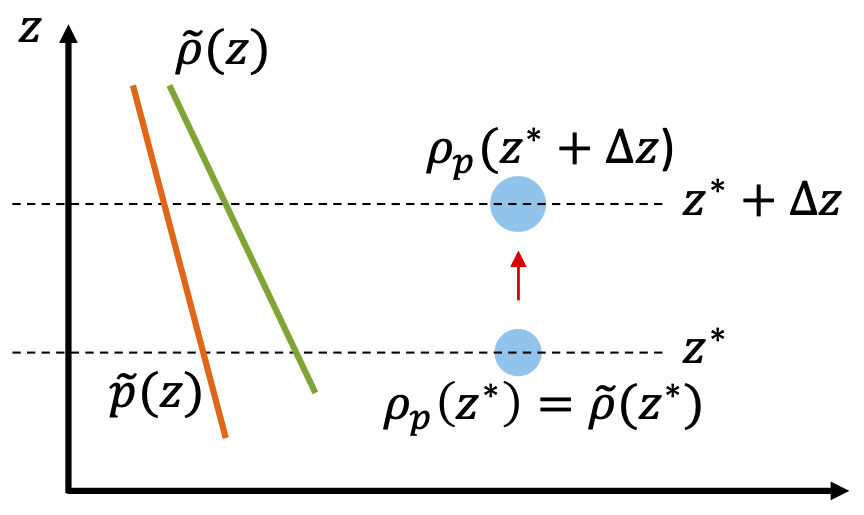
\includegraphics[width=0.5\textwidth,height=\textheight]{figures/Buoyfreq.png}

}

\caption{\label{fig-Buoyancy_parcel}A fluid parcel is raised from height
\(z^*\) to height \(z^* + \Delta z\) in a layer of hydrostatically
balanced fluid.}

\end{figure}

Consider a fluid at rest with density \(\tilde\rho(z)\) and hydrostatic
pressure \(\tilde p\), i.e., \(d\tilde p/dz = -g \tilde\rho\). Then
consider raising a parcel of fluid from a height \(z^*\) to
\(z^* + \Delta z\) (see Figure~\ref{fig-Buoyancy_parcel}). At \(z^*\),
the environment and the parcel are in hydrostatic balance and so \[
\frac{d\tilde p}{dz}\bigg |_{z^*} = -g \tilde\rho(z^*) = -g \rho_p(z^*),
\] where we denote by a subscript \(p\) a variable following the parcel
and a tilde denotes an environment variable.

The environment at \(z^*+\Delta z\) is also in hydrostatic balance: \[
\frac{d\tilde p}{dz}\bigg |_{z^*+\Delta z} = -g \tilde\rho(z^* +\Delta z).
\]

However, the fluid parcel at \(z^*+\Delta z\) is now being acted on by a
force given by \[
-\frac{d\tilde p}{dz}\bigg |_{z^*+\Delta z}  -g \rho_p(z^* +\Delta z)
\] since the pressure of the parcel is the same as the pressure of the
environment. Note the pressure gradient acts upwards and gravity
downwards. Then, since
\(-g \rho_p(z^* +\Delta z) \neq -g\tilde\rho(z^* +\Delta z) = {d\tilde p}/{dz}\bigg |_{z^*+\Delta z}\),
there is a net force acting on the fluid parcel (per unit volume) which
can be written as \begin{equation}\protect\hypertarget{eq-BuoForce}{}{
    F_b = g \tilde\rho(z^* +\Delta z) - g \rho_p( z^* +\Delta z)
}\label{eq-BuoForce}\end{equation}

We can then apply Newton's Second Law to the parcel at \(z^*+\Delta z\)
to give \[
    \rho_p(z^* +\Delta z) \frac{d^2 \Delta z}{dt^2} = F_b
\] and so \begin{equation}\protect\hypertarget{eq-N2Lparcel}{}{
\frac{d^2 \Delta z}{dt^2}  = \frac{g\left[ \tilde \rho(z^* +\Delta z) -  \rho_p( z^* +\Delta z) \right]}{\rho_p(z^* +\Delta z) }.
}\label{eq-N2Lparcel}\end{equation} Next, if we assume the density of
the parcel is conserved then we have that
\(\rho_p(z^* +\Delta z)=\rho_p(z^*)=\tilde\rho(z^*)\). Then we can write
Equation~\ref{eq-N2Lparcel} as \[
\frac{d^2 \Delta z}{dt^2}  = \frac{g\left[ \tilde \rho(z^* +\Delta z) -  \tilde\rho( z^*) \right]}{\tilde\rho(z^*) }\]
\begin{equation}\protect\hypertarget{eq-N2Lbuoyancy}{}{ \approx\frac{g}{\tilde\rho(z^*)}\frac{d\tilde\rho}{dz}\bigg |_{z^*}\Delta z }\label{eq-N2Lbuoyancy}\end{equation}
where we have used a Taylor series for \(\tilde\rho(z^* +\Delta z)\) to
arrive at the final expression. We see that if \({d\tilde\rho}/{dz}<0\)
then solutions to Equation~\ref{eq-N2Lbuoyancy} are oscillatory with
frequency \(N(z^*)\) where in general
\begin{equation}\protect\hypertarget{eq-BVfreq}{}{
N^2(z) = -\frac{g}{\tilde\rho}\frac{d\tilde\rho}{dz}.
}\label{eq-BVfreq}\end{equation} The quantity \(N(z)\) is known as the
\textbf{buoyancy frequency} or \textbf{Brunt--Väisälä} frequency. It
gives the theoretical frequency of vertical oscillations of a small
parcel of fluid in a stratified medium.

\begin{tcolorbox}[enhanced jigsaw, left=2mm, opacityback=0, coltitle=black, bottomtitle=1mm, title={Example}, toprule=.15mm, colbacktitle=quarto-callout-tip-color!10!white, breakable, arc=.35mm, titlerule=0mm, colback=white, toptitle=1mm, opacitybacktitle=0.6, rightrule=.15mm, bottomrule=.15mm, colframe=quarto-callout-tip-color-frame, leftrule=.75mm]

Consider a fluid parcel that is raised a distance \(\Delta z_0\) in a
fluid that is at rest. Find the motion of this parcel after it is let
go.

We assume that the displacement is small such that \(N = N_0\) remains
constant. To find the parcel dynamics we then need to solve
\begin{equation}\protect\hypertarget{eq-egBuoOscil}{}{
    \frac{d^2 \Delta z}{dt^2}  = - N_0^2 \Delta z, \quad \Delta z (t=0) = \Delta z_0, \quad \frac{d \Delta z}{dt}  (t=0) = 0. 
}\label{eq-egBuoOscil}\end{equation} The solution to this equation is \[
    \Delta z(t) = \Delta z_0 \cos{(N_0 t)},
\] which is a simple oscillatory motion with frequency \(N_0\).
Equation~\ref{eq-egBuoOscil} is very similar to the linear pendulum
equations. In pendulum motion, the restoring force is gravity, whereas
here the restoring force is buoyancy.

\end{tcolorbox}

\begin{tcolorbox}[enhanced jigsaw, toprule=.15mm, left=2mm, opacityback=0, breakable, arc=.35mm, colback=white, rightrule=.15mm, bottomrule=.15mm, colframe=quarto-callout-note-color-frame, leftrule=.75mm]
\begin{minipage}[t]{5.5mm}
\textcolor{quarto-callout-note-color}{\faInfo}
\end{minipage}%
\begin{minipage}[t]{\textwidth - 5.5mm}

If \({d\tilde\rho}/{dz}>0\) then \(N^2<0\) and the stratification is
\emph{unstable} meaning that if we raise a fluid parcel it will continue
to rise.

\end{minipage}%
\end{tcolorbox}

\begin{tcolorbox}[enhanced jigsaw, left=2mm, opacityback=0, coltitle=black, bottomtitle=1mm, title={Example}, toprule=.15mm, colbacktitle=quarto-callout-tip-color!10!white, breakable, arc=.35mm, titlerule=0mm, colback=white, toptitle=1mm, opacitybacktitle=0.6, rightrule=.15mm, bottomrule=.15mm, colframe=quarto-callout-tip-color-frame, leftrule=.75mm]

For a constant temperature atmosphere, we saw in an earlier example that
\(\tilde\rho = \rho_se^{-\frac{z}{H}}\) where
\(\rho_s = \frac{\rho_0}{\mathcal{R}T}\) and
\(H=\frac{\mathcal{R}T}{g}\). For this stratification,
\[ N^2 = -\frac{g}{\rho_se^{-\frac{z}{H}}}\left( -\frac{\rho_s}{H}e^{-\frac{z}{H}}\right) = \frac{g}{H}=\frac{g^2}{\mathcal{R}T}.\]
That is, \(N\) is independent of \(z\). With \(T=300K\),
\(N\approx 0.03s^{-1}\). Observations tell us that a more realistic
value for \(N\) is approximately \(0.01\mathrm{s^{-1}}\).

\end{tcolorbox}

\hypertarget{boussinesq-equations}{%
\section{Boussinesq equations}\label{boussinesq-equations}}

\hypertarget{density-and-temperature-variation-in-the-ocean-and-atmosphere}{%
\subsection{Density and temperature variation in the ocean and
atmosphere}\label{density-and-temperature-variation-in-the-ocean-and-atmosphere}}

\begin{figure}

{\centering 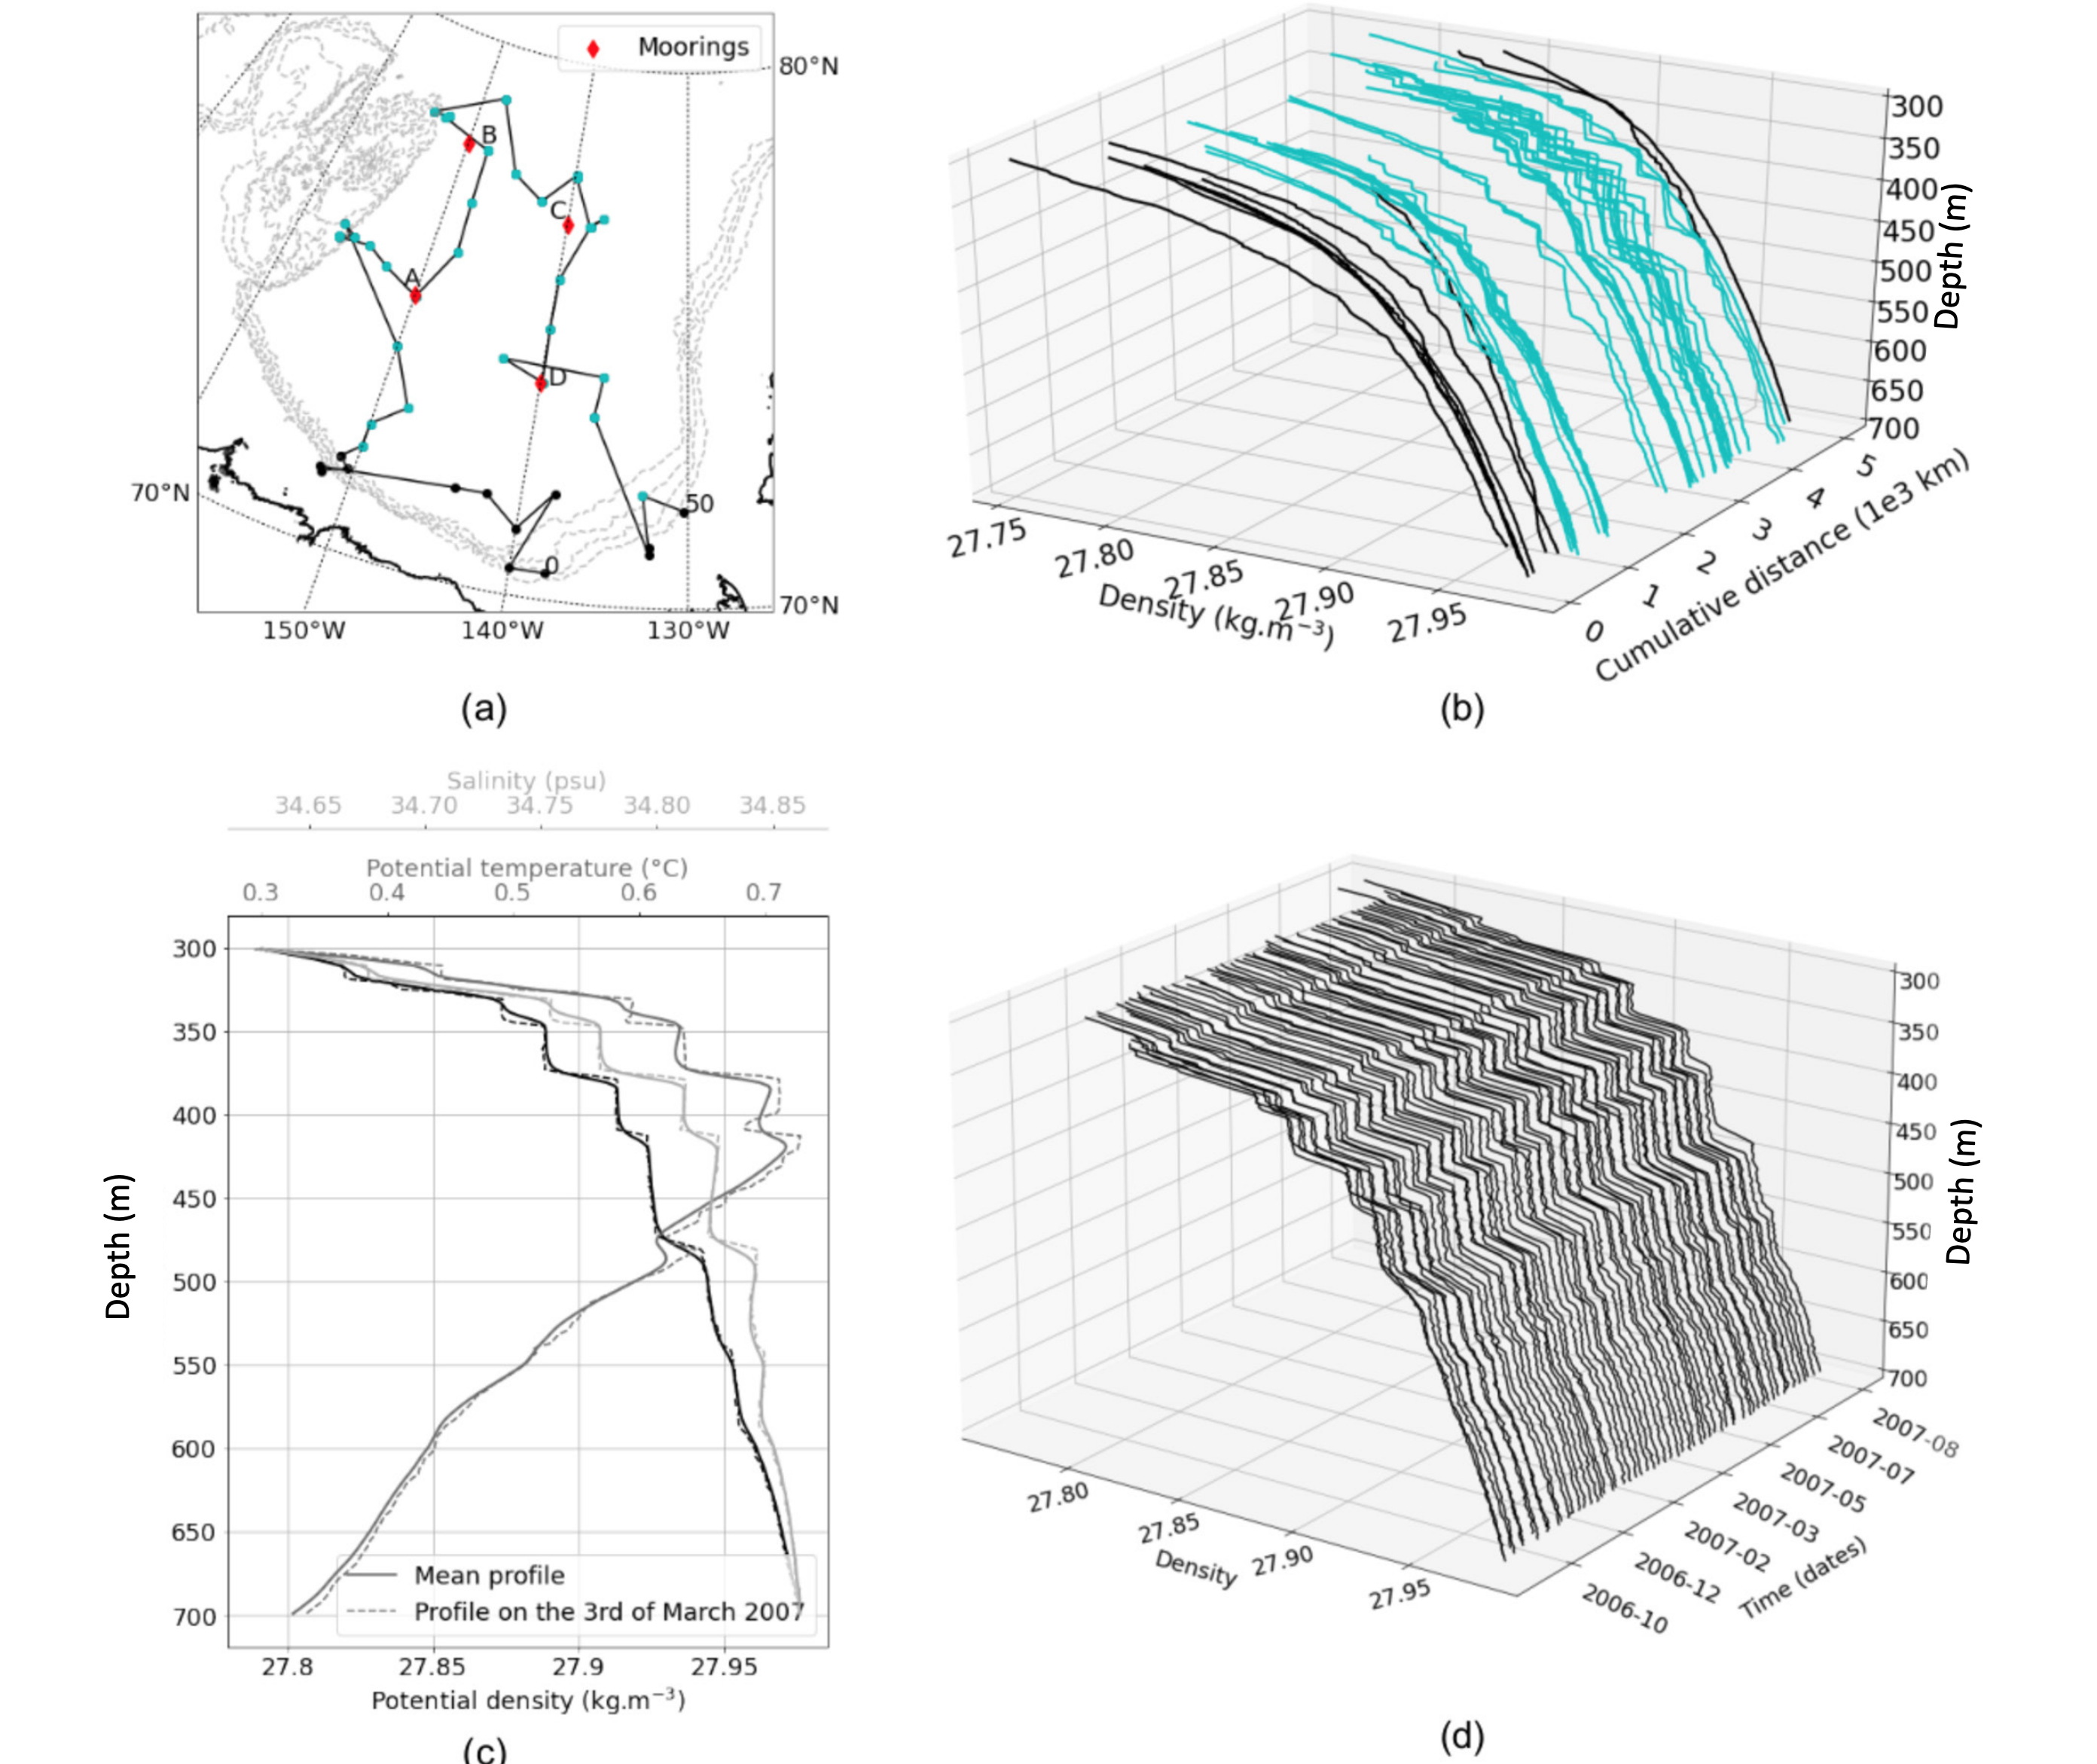
\includegraphics[width=1\textwidth,height=\textheight]{figures/densVarArcCorrected.png}

}

\caption{\label{fig-density_arctic}(a) Position of different
measurements in the Canada Basin of the Arctic Ocean. The trajectory
followed during the cruise is represented by the black lines between the
cast positions. (b) Density profiles from the 2006 survey within the
300--700\(\mathrm{m}\) depth range against distance traveled from the
first cast. Profiles in blue correspond to the blue dots in (a). (c)
Mean temperature and density profiles from mooring D averaged between
September 2006 and August 2007 are shown with solid lines. The dashed
lines show the same quantities but for a single cast in March 2007. (d)
Time evolution of the density profiles at mooring D shown in panel (a).
This figure is taken from (Menesguen et al.~2022).}

\end{figure}

In the lower atmosphere and most parts of the ocean, the density (or
temperature) does not change significantly at different horizontal
locations \(\xb=(x,y)\) or in time. This motivates the
\textbf{Boussinesq approximation} which involves writing the density
(and pressure) as a sum of a base profile plus small perturbation, where
the base profile only depends on \(z\). We will formulate this
approximation mathematically in the next section, but before that it
will be insightful to look at few observations of density and
temperature variations in the ocean and atmosphere.

Figure~\ref{fig-density_arctic} shows a combination of two types of
measurements in a region in the arctic ocean. In panel (a), there are
four red dots that are \textbf{mooring} measurements obtained by a
collection of devices connected to a wire and anchored on the sea floor.
The other dots are measurements taken by a cruise that sends diving
devices down into the ocean. The details of these observations are not
important for us, but they show that several locations are sampled by
different measuring devices and at different times. Panel (b) shows the
density profiles of the cruise measurements at different locations. It
is clear that the density profile has a (horizontal) mean that is a
function of \(z\). The perturbations to this mean by changing the
horizontal location are much smaller than the mean value itself. The
variation of density from the base profile is better quantified in the
panel (c). The solid black curve shows the mean (base) profile of the
density next to a single cast with dashed black curve, which marginally
deviates from the mean. Panel (d) shows the density profiles for a fixed
location (location D in panel (a)), but at different times. It can be
inferred from this plot that changing time does not affect the mean
density profile very much. Looking at different part of the ocean, we
get a more general base profile (a smoother mean). Nevertheless, the
underlying message of this example still holds: the density is well
approximated with a base profile that is a function of depth only plus
small perturbations.

\begin{figure}

{\centering 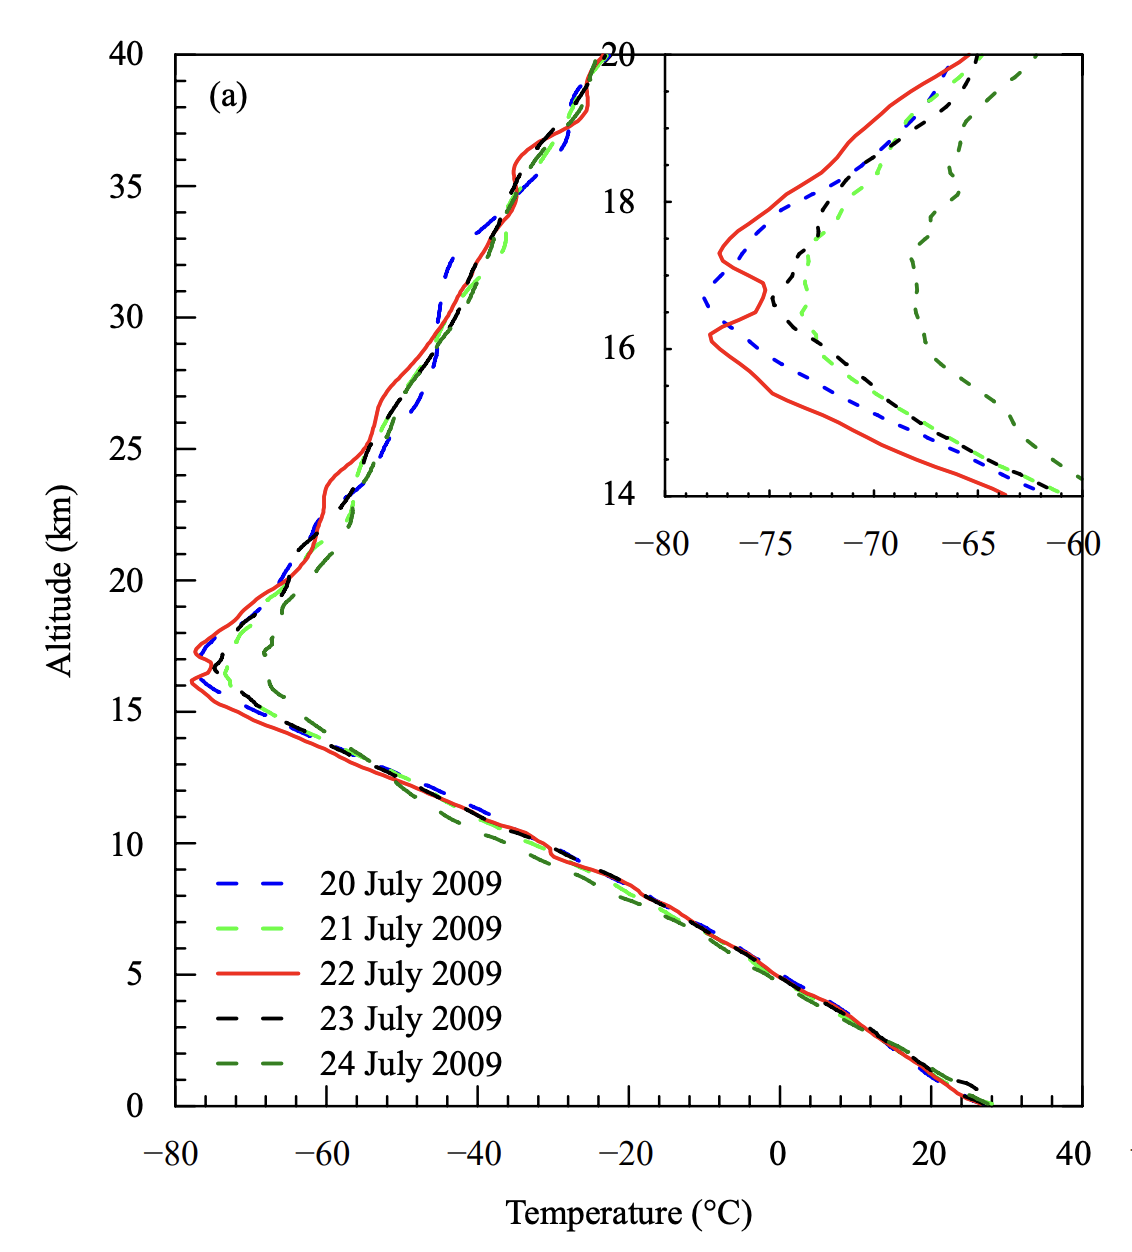
\includegraphics[width=0.5\textwidth,height=\textheight]{figures/TempProfileAtmos1.png}

}

\caption{\label{fig-atmos_Tprofile}An example of temperature-altitude
profiles of the daily averaged temperature up to 40 km from 20 to 24
July 2009 over the Indian region (65\(^{\circ}\)N--110\(^{\circ}\)E).
The figure is taken from (Prasad et al., 2018).}

\end{figure}

Figure~\ref{fig-atmos_Tprofile} displays the (daily) temperature
profiles over a region in India. Atmospheric temperature is directly
related to the density at each altitude (which has a fixed pressure).
Hence, the relative magnitude of the mean temperature to perturbations
can translate to the density as well. It is evident from this figure
that changes in temperature at each altitude are relatively small for
lower atmosphere (below 15km). There is a jump in temperature that is
known as ``tropopause''. Near the tropopause, the deviations from the
mean temperature profile are larger, and the Boussinesq approximation is
not justified.

Measurements similar to the examples just discussed are abundant in the
literature thanks to several decades of observational campaigns.
Considering them all together, we can conclude that in most parts of the
ocean, and in the lower atmosphere, the variations in density at a fixed
\(z\) are small relative to their means.

\hypertarget{boussinesq-approximation}{%
\subsection{Boussinesq approximation}\label{boussinesq-approximation}}

As we have seen, the density in the ocean and in the lower layer of
atmosphere varies by only a few percent across the depth or altitude. We
can therefore exploit the smallness of these variations and write \[
\rho(\xb,t) = \rho_0 + \delta\rho(\xb,t)
\] where \(\rho_0\) is the average density (a constant) and
\(\delta\rho\) are (small) perturbations away from this mean. The
perturbations are assumed small so that \(|\delta\rho|\ll\rho_0\).
Substituting this into the inviscid, incompressible momentum equation
(i.e., Equation~\ref{eq-incompmom} with \(\nu=0\)) and again assuming
gravity is the only body force acting so that \(\fb_b=-g\eb_z\), we find
\[
(\rho_0 + \delta\rho(\xb,t)) \frac{D\ub}{Dt} = -\nabla p - (\rho_0 + \delta\rho(\xb,t))g\eb_z.
\] Since \(|\delta\rho|\ll\rho_0\) we may be tempted to ignore all the
terms involving \(\delta\rho\). Instead, we neglect all the terms
involving \(\delta\rho\) \emph{except} in the term involving gravity
(here there is only one but in more complex cases there may be others).
This is because while \(|\delta\rho|\ll\rho_0\), gravity is strong and
so the buoyancy term (the one involving gravity) is retained. Making
this approximation, known as the \textbf{Boussinesq approximation},
leads to \[
\rho_0 \frac{D\ub}{Dt} = -\nabla p - (\rho_0 + \delta\rho(\xb,t))g\eb_z.
\] Then, dividing by \(\rho_0\) and combining with equation
(\ref{eq-incompdensity}) and (\ref{eq-divu0}), we obtain the so called
\textbf{Boussinesq equations}:
\begin{equation}\protect\hypertarget{eq-Bousmom}{}{\frac{\partial\ub}{\partial t} + (\ub\cdot\nabla)\ub = -\frac{1}{\rho_0}\nabla p -\frac{\rho}{\rho_0}g\eb_z. }\label{eq-Bousmom}\end{equation}
\begin{equation}\protect\hypertarget{eq-Bousdivu0}{}{ \nabla\cdot\ub = 0, }\label{eq-Bousdivu0}\end{equation}
\begin{equation}\protect\hypertarget{eq-Bousdensity}{}{\frac{D\rho}{Dt}  = \frac{\partial \rho}{\partial t} + (\ub\cdot\nabla)\rho= 0, }\label{eq-Bousdensity}\end{equation}

\begin{tcolorbox}[enhanced jigsaw, toprule=.15mm, left=2mm, opacityback=0, breakable, arc=.35mm, colback=white, rightrule=.15mm, bottomrule=.15mm, colframe=quarto-callout-note-color-frame, leftrule=.75mm]
\begin{minipage}[t]{5.5mm}
\textcolor{quarto-callout-note-color}{\faInfo}
\end{minipage}%
\begin{minipage}[t]{\textwidth - 5.5mm}

Although we have derived this set of Boussinesq equations starting from
the assumption of an incompressible fluid, it is possible to show that
the Boussinesq approximation applies to a more general compressible
fluid.

\end{minipage}%
\end{tcolorbox}

\begin{tcolorbox}[enhanced jigsaw, toprule=.15mm, left=2mm, opacityback=0, breakable, arc=.35mm, colback=white, rightrule=.15mm, bottomrule=.15mm, colframe=quarto-callout-note-color-frame, leftrule=.75mm]
\begin{minipage}[t]{5.5mm}
\textcolor{quarto-callout-note-color}{\faInfo}
\end{minipage}%
\begin{minipage}[t]{\textwidth - 5.5mm}

The Boussineq approximation is valid everywhere in the ocean since
density variations are small. However, it is also valid for any motions
in the atmosphere that are confined to a layer that is thin compared
with the scale height of the atmosphere. For the Earth's atmosphere, we
have seen that the scale height is approximately \(8\)km and so the
Boussinesq approximation should apply to motions that are confined to
layers of about \(1\)km or less.

\end{minipage}%
\end{tcolorbox}

\hypertarget{buoyancy-as-a-variable}{%
\subsection{Buoyancy as a variable}\label{buoyancy-as-a-variable}}

Next, let's consider splitting our variables into a reference state and
perturbations to this state. We will consider a static, time-independent
reference state with a vertical density stratification
\(\rho=\tilde\rho(z)\). Equation~\ref{eq-Bousdivu0} and
Equation~\ref{eq-Bousdensity} are automatically satisfied by this
reference state and Equation~\ref{eq-Bousmom} demands
\begin{equation}\protect\hypertarget{eq-hydrobal2}{}{
p=\tilde p(z) \quad \text{with} \quad \frac{d\tilde p}{dz} = -\tilde\rho g. 
}\label{eq-hydrobal2}\end{equation} Decomposing our variables in this
way gives \begin{equation}\protect\hypertarget{eq-decompvar}{}{
\ub = \ub'(\xb,t), \quad \rho = \tilde\rho(z) + \rho'(\xb,t), \quad p = \tilde p(z) + p'(\xb,t) 
}\label{eq-decompvar}\end{equation} where a tilde denotes a reference
state variable and the primed quantities are perturbations to these
states (for now no assumptions are made about the size of the
perturbations).

Now, substituting (\ref{eq-decompvar}) into Equation~\ref{eq-Bousmom}
gives \[
    \frac{\partial\ub'}{\partial t} + (\ub'\cdot\nabla)\ub' = -\frac{1}{\rho_0}\nabla p' -\frac{\rho'}{\rho_0}g\eb_z = -\frac{1}{\rho_0}\nabla p' +b\eb_z, 
\] where we have used Equation~\ref{eq-hydrobal2} to cancel reference
state terms and introduced the \emph{buoyancy} variable
\begin{equation}\protect\hypertarget{eq-buoyance_Variable}{}{ b = -\frac{\rho'}{\rho_0} g .
}\label{eq-buoyance_Variable}\end{equation} Note that this expression is
analogous to the buoyancy force per unit mass \(F_b/\rho_0\) introduced
in Equation~\ref{eq-BuoForce}.

Substituting (\ref{eq-decompvar}) into Equation~\ref{eq-Bousdivu0}
simply gives \(\nabla\cdot\ub'=0\). Finally, substituting
(\ref{eq-decompvar}) into Equation~\ref{eq-Bousdensity} gives \[
\frac{\partial(\tilde \rho(z)+\rho')}{\partial t} + (\ub'\cdot\nabla)(\tilde\rho(z)+\rho')=0\]
\begin{equation}\protect\hypertarget{eq-rhoprimed}{}{\Rightarrow \frac{\partial\rho'}{\partial t} + (\ub'\cdot\nabla)\rho' + w'\frac{d\tilde\rho}{dz}=0.}\label{eq-rhoprimed}\end{equation}
Multiplying Equation~\ref{eq-rhoprimed} by \(-\frac{g}{\rho_0}\) allows
us to form \begin{align*}
 \frac{Db}{Dt}+\left(\frac{-g}{\rho_0}\frac{d\tilde\rho}{dz}\right)w'&=0,\\
 \Rightarrow\frac{Db}{Dt}+N^2(z)w'&=0
\end{align*} where \[
N^2(z) = -\frac{g}{\rho_0}\frac{d\tilde\rho}{dz}.
\] Here \(N(z)\) is the buoyancy frequency in the Boussinesq
approximation. Note it is subtly different to the definition in
Equation~\ref{eq-BVfreq}.

Gathering together the Boussinesq equations for the perturbation
quantities we have the following equation set:

\begin{tcolorbox}[enhanced jigsaw, left=2mm, opacityback=0, coltitle=black, bottomtitle=1mm, title={\textbf{(Non-hydrostatic) Boussinesq Equations}}, toprule=.15mm, colbacktitle=quarto-callout-important-color!10!white, breakable, arc=.35mm, titlerule=0mm, colback=white, toptitle=1mm, opacitybacktitle=0.6, rightrule=.15mm, bottomrule=.15mm, colframe=quarto-callout-important-color-frame, leftrule=.75mm]

\begin{equation}\protect\hypertarget{eq-Bousmombuoy}{}{ \frac{\partial\ub}{\partial t} + (\ub\cdot\nabla)\ub = -\frac{1}{\rho_0}\nabla p +b\eb_z, }\label{eq-Bousmombuoy}\end{equation}
\begin{equation}\protect\hypertarget{eq-Bousdivu0buoy}{}{\nabla\cdot\ub=0,  }\label{eq-Bousdivu0buoy}\end{equation}
\begin{equation}\protect\hypertarget{eq-Bousdenistybuoy}{}{\frac{\partial b}{\partial t}+(\ub\cdot\nabla)b+N^2(z)w=0,}\label{eq-Bousdenistybuoy}\end{equation}

\end{tcolorbox}

where we have dropped the primes from perturbation quantities as is
customary.

\begin{tcolorbox}[enhanced jigsaw, toprule=.15mm, left=2mm, opacityback=0, breakable, arc=.35mm, colback=white, rightrule=.15mm, bottomrule=.15mm, colframe=quarto-callout-note-color-frame, leftrule=.75mm]
\begin{minipage}[t]{5.5mm}
\textcolor{quarto-callout-note-color}{\faInfo}
\end{minipage}%
\begin{minipage}[t]{\textwidth - 5.5mm}

Note here that \(p\) is a perturbation to the background pressure state.
In general, when \(p\) appears along side buoyancy in the governing
equations then this indicates it is a perturbation pressure. This is in
contrast to the Boussinesq equations where \(p\) in
Equation~\ref{eq-Bousmom} is taken to mean the full pressure (likewise
in Equation~\ref{eq-Bousmom}, \(\rho\) is the full density).

\end{minipage}%
\end{tcolorbox}

\begin{tcolorbox}[enhanced jigsaw, left=2mm, opacityback=0, coltitle=black, bottomtitle=1mm, title={Example}, toprule=.15mm, colbacktitle=quarto-callout-tip-color!10!white, breakable, arc=.35mm, titlerule=0mm, colback=white, toptitle=1mm, opacitybacktitle=0.6, rightrule=.15mm, bottomrule=.15mm, colframe=quarto-callout-tip-color-frame, leftrule=.75mm]

The buoyancy (Brunt--Väisälä) frequency that appears in
Equation~\ref{eq-Bousdenistybuoy} is an important quantity in different
regimes of geophysical flows. Figure~\ref{fig-Nprofile} shows the values
of \(N^2\) for a region in the atmosphere/ocean as functions of
altitude/depth. In the left plot, \(N^2\) over the region of Gadanki in
India is shown. There is a noticeable jump at around 18km altitude
(similar to what we observed in figure Figure~\ref{fig-atmos_Tprofile},
marking the ``tropopause'', which is the border between two layers of
atmosphere (troposphere and stratosphere). Note that the height of
tropopause varies to some degrees in different locations (that is why
the jump in Figure~\ref{fig-atmos_Tprofile} and
Figure~\ref{fig-Nprofile} appears at slightly different altitudes).
Around the tropopause, constant \(N\) or even the Boussinesq
approximation are not valid, but in the lower atmosphere (below the
tropopause) \(N\) can be assumed constant. Horizontal bars show standard
deviations obtained while considering 43 different measurements during
April 2006 to March 2007. The low variability in the lower atmosphere
(relatively small bars) justifies the Boussinesq approximation, whereas
the high variability near tropopause shows this approximation is no
longer valid around this altitude.

The right plot is obtained from a mooring observation (``NISKINe''
campaign). For the deep ocean (lower than 800 meters), it is safe to use
constant \(N\). However, in the upper ocean the variation of \(N\) with
depth cannot be neglected. A comparison between the two figures shows
that \(N\) is an order of magnitude smaller in the ocean.

\begin{figure}[H]

\begin{minipage}[t]{0.50\linewidth}

{\centering 

\raisebox{-\height}{

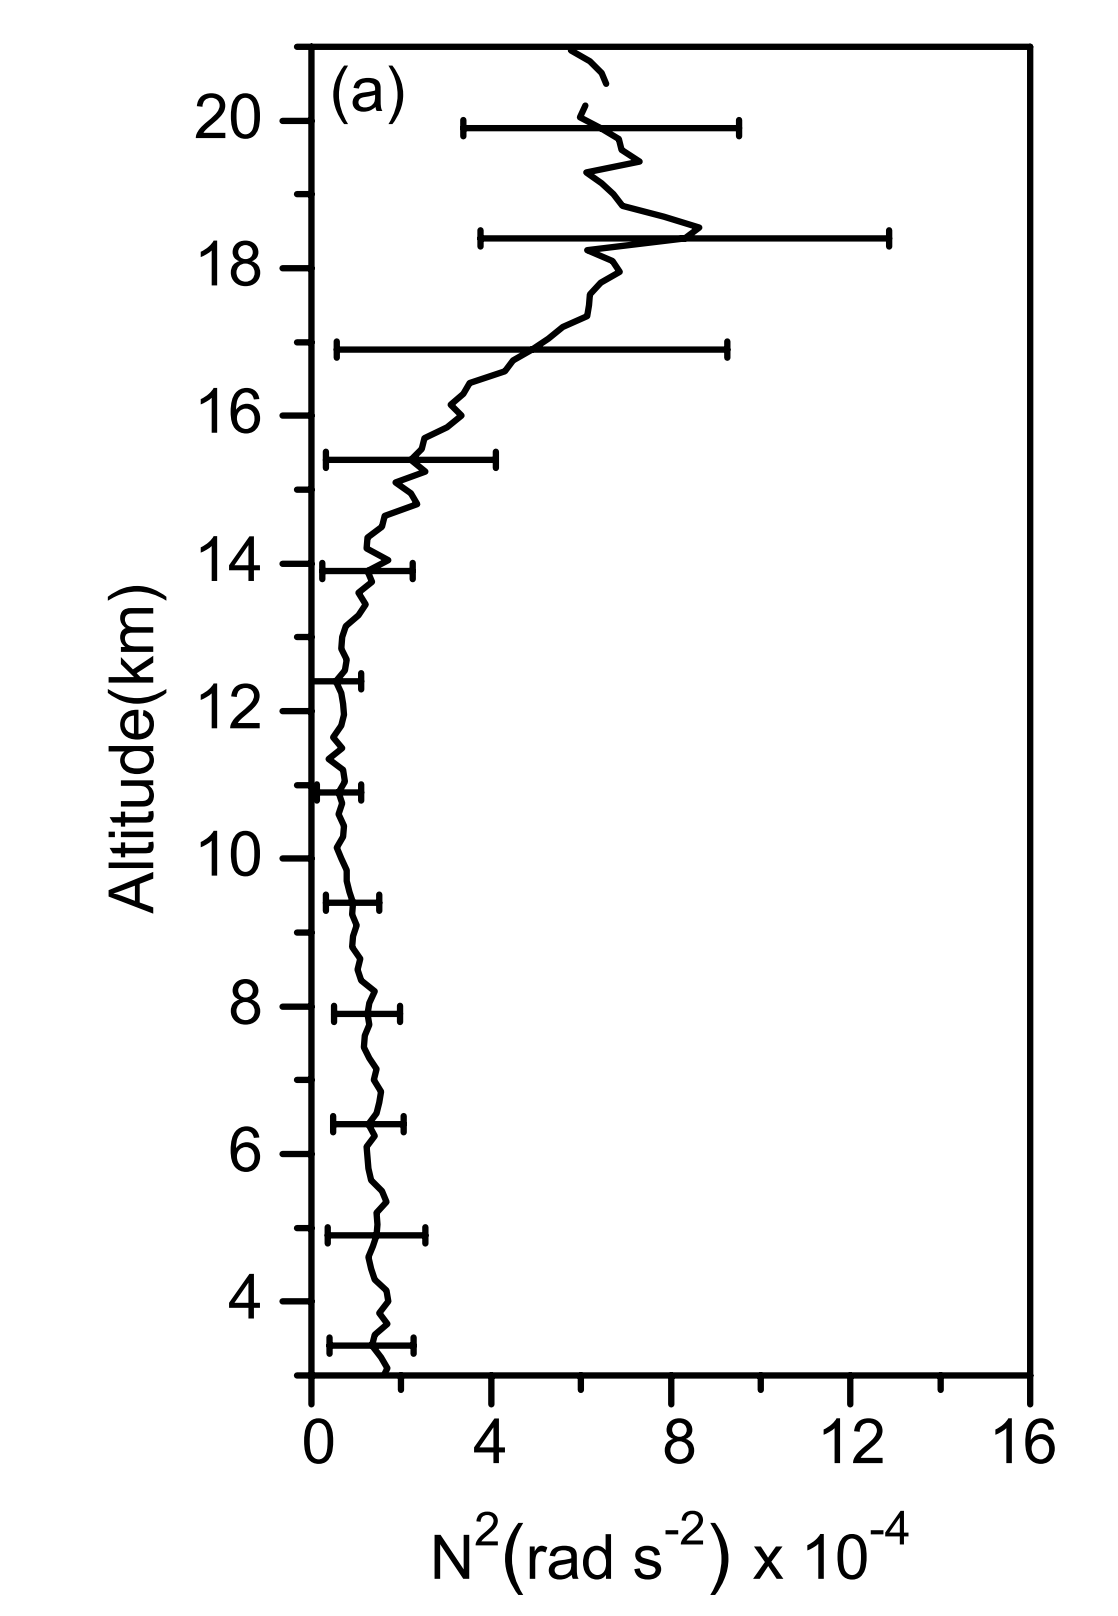
\includegraphics{figures/N2atmosphere.png}

}

}

\end{minipage}%
%
\begin{minipage}[t]{0.50\linewidth}

{\centering 

\raisebox{-\height}{

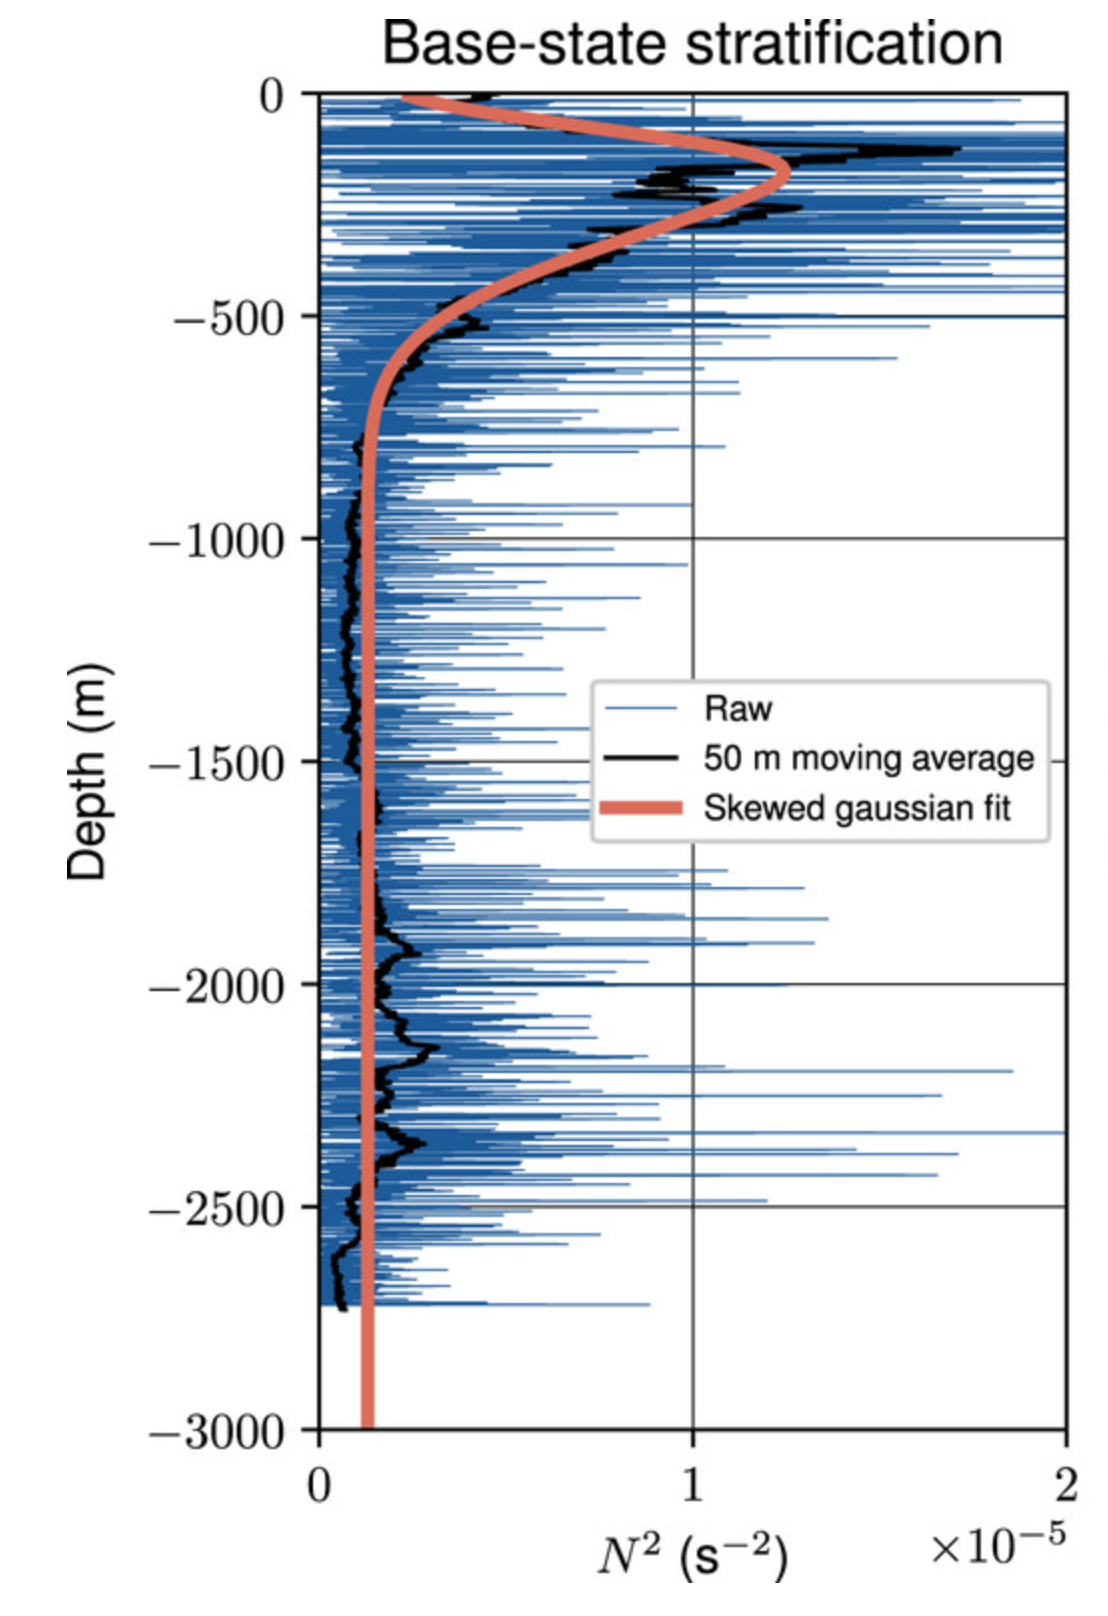
\includegraphics{figures/N2profile_ocean.png}

}

}

\end{minipage}%

\caption{\label{fig-Nprofile}Left: Stratification in the atmosphere in
the region of Gadanki in India (13.5\(^{\circ}\)N, 79.2\(^{\circ}\)E).
This curve is obtained by averaging over 43 radar measurements and the
bars show the standard deviation for each altitude. This plot is taken
from (Mehta et al., 2008). Right: raw stratification profile (blue)
observed during a pilot cruise measurement campaign named ``NISKINe'',
along with its 50-m moving average (black) and a Gaussian fit (orange).
This plot is taken from (Asselin \& Young, 2020).}

\end{figure}

\end{tcolorbox}

\hypertarget{sec-hydroapprox}{%
\subsection{Hydrostatic approximation}\label{sec-hydroapprox}}

A common approximation in geophysical fluid dynamics is to assume that
the horizontal scale is large compared to the vertical scale. In this
case, the vertical component of the momentum equation is simply replaced
by our hydrostatic balance equation. This is known as the
\emph{hydrostatic approximation} and leads to the following
\textbf{hydrostatic Boussinesq equations}

\begin{tcolorbox}[enhanced jigsaw, left=2mm, opacityback=0, coltitle=black, bottomtitle=1mm, title={\textbf{(Hydrostatic) Boussinesq Equations}}, toprule=.15mm, colbacktitle=quarto-callout-important-color!10!white, breakable, arc=.35mm, titlerule=0mm, colback=white, toptitle=1mm, opacitybacktitle=0.6, rightrule=.15mm, bottomrule=.15mm, colframe=quarto-callout-important-color-frame, leftrule=.75mm]

\begin{equation}\protect\hypertarget{eq-BoussinesqHydrostat1}{}{ \frac{\partial \vb}{\partial t} + (\ub\cdot\nabla)\vb = -\frac{1}{\rho_0}\nabla_H p,}\label{eq-BoussinesqHydrostat1}\end{equation}
\begin{equation}\protect\hypertarget{eq-hydroapprox_hydrobal}{}{   \frac{\partial p}{\partial z}  = \rho_0 b = -\rho g,}\label{eq-hydroapprox_hydrobal}\end{equation}
\begin{equation}\protect\hypertarget{eq-BoussinesqHydrostat3}{}{   \nabla\cdot \ub =0,}\label{eq-BoussinesqHydrostat3}\end{equation}
\begin{equation}\protect\hypertarget{eq-BoussinesqHydrostat4}{}{    \frac{\partial b}{\partial t} + (\ub\cdot\nabla)b +N^2w =0,}\label{eq-BoussinesqHydrostat4}\end{equation}

\end{tcolorbox}

where \(\vb=(u,v)\) is the horizontal velocity and
\(\nabla_H=\left(\frac{\partial}{\partial x}, \frac{\partial}{\partial y}\right)\).

Note that the hydrostatic approximation has resulted in the vertical
momentum equation being replaced by hydrostatic balance.

\begin{tcolorbox}[enhanced jigsaw, toprule=.15mm, left=2mm, opacityback=0, breakable, arc=.35mm, colback=white, rightrule=.15mm, bottomrule=.15mm, colframe=quarto-callout-note-color-frame, leftrule=.75mm]
\begin{minipage}[t]{5.5mm}
\textcolor{quarto-callout-note-color}{\faInfo}
\end{minipage}%
\begin{minipage}[t]{\textwidth - 5.5mm}

The Boussinesq equations (\ref{eq-Bousmombuoy}) -
(\ref{eq-Bousdenistybuoy}) (and their hydrostatic counterparts
(\ref{eq-BoussinesqHydrostat1}) - (\ref{eq-BoussinesqHydrostat4})) are
the fundamental equations that are solved numerically in weather
forecast and climate models. Because we observe and measure everything
from the rotating Earth, these equations are solved in the rotating
frame of reference (which we will come to in
Chapter~\ref{sec-chap:rotation}). Most climate models use the
Hydrostatic equations as they require far fewer computational resources.
Hence, because climate models (unlike weather models) are run for very
long times (several years or decades), it is worth reducing the
computational cost at the expense of making the hydrostatic assumption.

\end{minipage}%
\end{tcolorbox}

\begin{tcolorbox}[enhanced jigsaw, toprule=.15mm, left=2mm, opacityback=0, breakable, arc=.35mm, colback=white, rightrule=.15mm, bottomrule=.15mm, colframe=quarto-callout-note-color-frame, leftrule=.75mm]
\begin{minipage}[t]{5.5mm}
\textcolor{quarto-callout-note-color}{\faInfo}
\end{minipage}%
\begin{minipage}[t]{\textwidth - 5.5mm}

In the geophysical fluids literature, equations
(\ref{eq-BoussinesqHydrostat1}) - (\ref{eq-BoussinesqHydrostat4}) are
often known as the \emph{primitive equations}. This is somewhat
confusing as the non-Hydrostatic Boussinesq equation set is more
general. However, the Hydrostatic Boussinesq equations are still more
accurate than some other reduced equations such as the shallow water
equations and quasigeostrophic equations that we will study in Chapters
\ref{sec-chap:SW} and \ref{sec-Geostrophic}, respectively.

\end{minipage}%
\end{tcolorbox}

\hypertarget{sec-chap:SW}{%
\chapter{Shallow Water Systems}\label{sec-chap:SW}}

\hypertarget{overview-1}{%
\section{Overview}\label{overview-1}}

The shallow water equations are a model of a thin layer of fluid with
constant density which is bounded by a rigid surface from below and by a
free surface from above. By ``thinness'' -- which is the most defining
feature of these fluids -- we mean the horizontal length scales of these
flows are much larger than their vertical scales (and hence the name
shallow!). Other characteristics of these equations which we will
discuss in this section are the direct consequence of the thinness and
constant density assumptions.

The shallow water equations are one of the simplest sets of PDEs
describing geophysical fluids, yet they are very useful. They are used
in practical models of shallow lakes, rivers and coastal flows. Due to
their relative simplicity, many theoretical concepts in geophysical
fluid dynamics are first investigated for shallow water systems before
being studied in more complex systems. They also incorporate many
phenomena that characterise atmospheric and oceanic flows such as
geostrophic balance and waves (we will discuss these later in the
course). The practical importance of shallow water equations aside,
their derivation is a good example of using rigorous mathematical steps
and physical assumptions to reduce the Boussinsq equations to a much
simpler set.

\hypertarget{derivation}{%
\section{Derivation}\label{derivation}}

We use the defining characteristics of shallow water flows to derive
their governing equations. Before that, let's clarify the notation and
conventions we are going to use (this is sometimes the most confusing
part about shallow water systems because different sources in the
literature adopt very different notation). We assume the \(z\) axis is
perpendicular to the layer of water as shown in
Figure~\ref{fig-SW_schematic}. \(z=0\) can be placed at any arbitrary
level (naturally we want to see it close the bottom surface).
\(\eta(x,y,t)\) is the vertical position of fluid surface measured from
\(z=0\). Likewise, \(\eta_b(x,y,t)\) is the vertical height of bottom
topography measured from \(z=0\). \(h(x,y,t)\) is the thickness of water
column measured from bottom boundary all the way to free surface,
i.e.~\(h = \eta - \eta_b\). The thinness of fluid has an important
consequence: the vertical velocity (in the \(z\) direction) is much
smaller than the horizontal velocity components (but is not necessarily
zero). Hence, we only consider the two-dimensional horizontal velocity
denoted by \(\vb =(u,v)\) and assume \(w \ll u, v\). Lastly, we denote
the horizontal gradient operator by
\(\gradH = (\partial / \partial x, \partial / \partial y)\).

\begin{figure}

{\centering 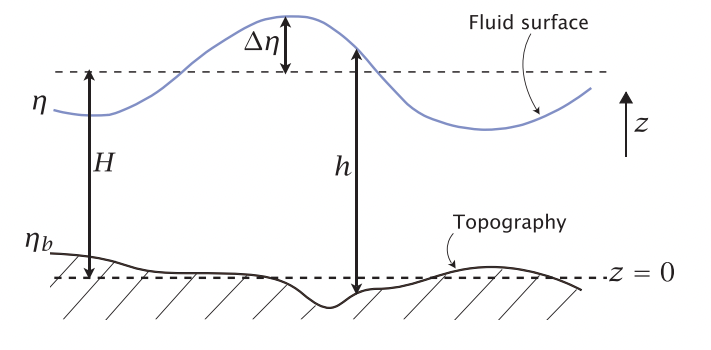
\includegraphics[width=0.7\textwidth,height=\textheight]{figures/SWschematic.png}

}

\caption{\label{fig-SW_schematic}A shallow water system. \(h\) is the
thickness of a water column, \(H\) is the mean thickness, \(\eta\) is
the height of the free surface and \(\eta_b\) is the height of the lower
rigid. \(\Delta \eta\) is the deviation of free from average height.}

\end{figure}

\hypertarget{momentum-equations}{%
\subsection{Momentum equations}\label{momentum-equations}}

One of the main consequences of small vertical velocity appears in the
vertical momentum equation. Let's consider the vertical momentum
equation in the Boussinesq system (i.e., Equation~\ref{eq-Bousmom})
\begin{equation}\protect\hypertarget{eq-verticalBous}{}{ \frac{\partial w}{\partial t} + (\vb \cdot\gradH)w + w \frac{\partial w}{\partial z} = -\frac{1}{\bar\rho} \frac{\partial p}{\partial z} -\frac{\rho}{\bar\rho}g. 
}\label{eq-verticalBous}\end{equation} Assuming \(w\) to be smaller than
the other variables, the vertical momentum equation then reduces to \[
    \frac{\partial p}{\partial z} = - \rho g,  
\] which is simply the hydrostatic balance that was discussed in
Section~\ref{sec-hydrostat} (cf. Equation~\ref{eq-hydrobal}). Because
the density is assumed constant (\(\rho = \rho_0\)), we may integrate
this equation from \(\eta\) to an arbitrary height \(z\) to give
\begin{equation}\protect\hypertarget{eq-integrated_pressure}{}{ p(x,y,z,t) - p(x,y,\eta(x,y,t),t) = \rho_0 g (\eta(x,y,t) - z).
}\label{eq-integrated_pressure}\end{equation} It is physically justified
to assume the pressure at the free surface \(p(x,y,\eta,t)\) is constant
(for some applications we may need to change this assumption though).
Hence, we can take the horizontal gradient of both sides of
Equation~\ref{eq-integrated_pressure} to arrive at
\begin{equation}\protect\hypertarget{eq-grad_p-eta}{}{ \gradH \ p = \rho_0 g \ \gradH \ \eta.
}\label{eq-grad_p-eta}\end{equation} Now we consider the horizontal
momentum equation in Equation~\ref{eq-Bousmom} and substitute for the
horizontal pressure gradient using Equation~\ref{eq-grad_p-eta}
\begin{equation}\protect\hypertarget{eq-SWmomn1}{}{ \frac{\partial \vb}{\partial t} + (\vb \cdot\gradH) \vb =  - g \ \gradH \ \eta,
}\label{eq-SWmomn1}\end{equation} where we also neglected the vertical
velocity at leading order. Note that the right-hand side of this
equation is independent of \(z\). Hence, if we assume the velocity is
initially independent of \(z\), it should remain independent of \(z\),
i.e. \(\vb = \vb(x,y,t)\). As a consequence, for the rest of this
chapter we do not deal with \(z\) derivative. We also simplify the
notation by replacing \(\gradH\) with \(\grad\) in the context of
shallow water equation since there is no \(z\) dependence. For example,
we write Equation~\ref{eq-SWmomn1} as
\begin{equation}\protect\hypertarget{eq-SWmomn1}{}{
    \frac{D \vb}{D t}  =  - g \ \grad \eta.
}\label{eq-SWmomn1}\end{equation}

Note that for three-dimensional flows such as those described by the
Boussinesq equations, we still distinguish between horizontal and
three-dimensional gradient and show them with \(\gradH\) and \(\grad\),
respectively.

\hypertarget{mass-continuity-equation}{%
\subsection{Mass continuity equation}\label{mass-continuity-equation}}

\begin{figure}

{\centering 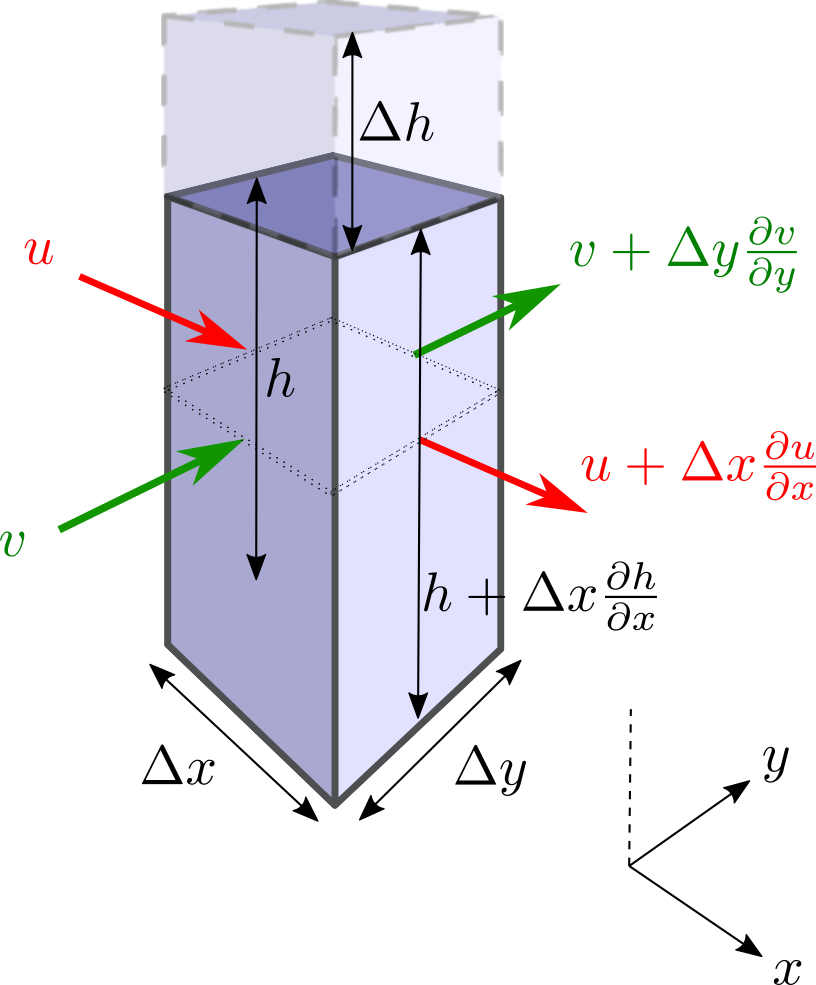
\includegraphics[width=0.4\textwidth,height=\textheight]{figures/SHcolumn.png}

}

\caption{\label{fig-SW_column}A column of fluid in shallow water.}

\end{figure}

Consider a (Cartesian) column of shallow water as shown in
Figure~\ref{fig-SW_column}. The height of this column \(h\) is measured
from the bottom boundary to the free surface. The cross-sectional area
of this column is \(\Dl x \Dl y\). If the fluid enters this column from
the sides, its height has to increase to conserve mass (note that the
density is constant and the fluid is incompressible). More
quantitatively, let's consider the two sides perpendicular to the
\(x\)-axis. If the velocity normal to one of the sides is \(u\), the
normal velocity to the other side will be
\(u + \Dl x \ {\partial u} / {\partial x}\) (see
Figure~\ref{fig-SW_column}). Likewise, If the thickness of one side is
\(h\), the thickness of the other side will be
\(h + \Dl x \ {\partial h} / {\partial x}\). The mass flux through a
side is calculated as the normal velocity times the surface area of the
side times density. For example, if the normal velocity and vertical
thickness are \(u\) and \(h\) respectively, the mass flux will be
\(\rho_0 u h \Dl y\) (without loss of generality we assume the velocity
\(u\) is pointing inward). Hence, the total amount of mass
entering/leaving from these two sides is

\begin{align*}
 \text{MF}_x = \text{mass flux along} &\text{ the $x$ axis} = \rho_0 u h \Dl y - \rho_0 \left( u + \Dl x \ \frac{\partial u}{\partial x} \right)  \left(h + \Dl x \ \frac{\partial h}{\partial x} \right) \Dl y \\
   &= -\rho_0 \Dl x \ \frac{\partial u}{\partial x}  h \Dl y
    -\rho_0 u \ \Dl x \  \frac{\partial h}{\partial x}   \Dl y  
    -\rho_0 \Dl x \ \frac{\partial u}{\partial x} \Dl x \ \frac{\partial h}{\partial x}  \Dl y 
    \end{align*} Likewise, we obtain the total mass flux along the \(y\)
axis \[        \text{MF}_y 
    = -\rho_0 \Dl y \ \frac{\partial v}{\partial y}  h \Dl x
    -\rho_0 v \ \Dl y \  \frac{\partial h}{\partial y}   \Dl x
    -\rho_0 \Dl y \ \frac{\partial v}{\partial y} \Dl y \ \frac{\partial h}{\partial y}  \Dl x 
\] The rate of change of mass in this fluid column is
\(\rho_0 \Dl x \Dl y \Dl h / \Dl t\) which should be equal to mass flux
from the sides, i.e., \[
    \rho_0 \Dl x \Dl y  \frac{\Dl h }{\Dl t } =  \text{MF}_x +  \text{MF}_y. 
\] After dividing this equation by \(\rho_0 \Dl x \Dl y\) and taking the
limit as \(\Dl x, \Dl y, \Dl t \to 0\), we find \[
    \frac{\partial h}{\partial t} = - h \left( \frac{\partial u}{\partial x} +\frac{\partial v}{\partial y} \right) - u  \frac{\partial h}{\partial x} - v  \frac{\partial h}{\partial y} 
\] which can be written as
\begin{equation}\protect\hypertarget{eq-SWmass}{}{
    \frac{\partial h}{\partial t} + \gradH \cdot (h \vb)=0, \quad \text{or} \quad  \frac{D h}{D t} + h \gradH \cdot \vb=0.
}\label{eq-SWmass}\end{equation} Note that unlike Boussinesq or
incompressible flows, the shallow water velocity is not divergence free.
This is because the columns of fluids can be compressed by increasing
their height.

\begin{tcolorbox}[enhanced jigsaw, toprule=.15mm, left=2mm, opacityback=0, breakable, arc=.35mm, colback=white, rightrule=.15mm, bottomrule=.15mm, colframe=quarto-callout-note-color-frame, leftrule=.75mm]
\begin{minipage}[t]{5.5mm}
\textcolor{quarto-callout-note-color}{\faInfo}
\end{minipage}%
\begin{minipage}[t]{\textwidth - 5.5mm}

The conservation of mass equation for the shallow water system can be
derived from 3D mass conservation equation using \(w \ll u, v\) (see the
assignments).

\end{minipage}%
\end{tcolorbox}

In summary, in a non-rotating frame, the inviscid shallow water
equations are

\begin{tcolorbox}[enhanced jigsaw, left=2mm, opacityback=0, coltitle=black, bottomtitle=1mm, title={\textbf{Inviscid Shallow Water Equations}}, toprule=.15mm, colbacktitle=quarto-callout-important-color!10!white, breakable, arc=.35mm, titlerule=0mm, colback=white, toptitle=1mm, opacitybacktitle=0.6, rightrule=.15mm, bottomrule=.15mm, colframe=quarto-callout-important-color-frame, leftrule=.75mm]

\begin{equation}\protect\hypertarget{eq-SW1}{}{ \text{momentum:} \quad \frac{D \vb}{D t}  =  - g \ \gradH \eta. }\label{eq-SW1}\end{equation}
\begin{equation}\protect\hypertarget{eq-SW2}{}{ \text{mass continuity:} \quad \frac{\partial h}{\partial t} + \gradH \cdot (h \vb) = 0, \quad \text{or} \quad  \frac{D h}{D t} + h \gradH \cdot \vb=0 }\label{eq-SW2}\end{equation}
\begin{equation}\protect\hypertarget{eq-SW3}{}{ \text{height relation:}  \quad  h(x,y,t) = \eta(x,y,t) - \eta_b(x,y,t). }\label{eq-SW3}\end{equation}

\end{tcolorbox}

\begin{tcolorbox}[enhanced jigsaw, left=2mm, opacityback=0, coltitle=black, bottomtitle=1mm, title={Example}, toprule=.15mm, colbacktitle=quarto-callout-tip-color!10!white, breakable, arc=.35mm, titlerule=0mm, colback=white, toptitle=1mm, opacitybacktitle=0.6, rightrule=.15mm, bottomrule=.15mm, colframe=quarto-callout-tip-color-frame, leftrule=.75mm]

\begin{figure}[H]

{\centering 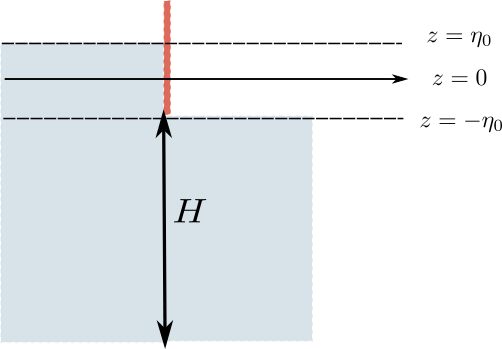
\includegraphics[width=0.4\textwidth,height=\textheight]{figures/SWdambreak.png}

}

\caption{\label{fig-SW_dambreak}A schematic figure of dam break with two
levels of water on each side.}

\end{figure}

Let's consider an example of a dam or membrane that creates two levels
of fluid as shown in the figure Figure~\ref{fig-SW_dambreak}. The fluid
is initially at rest and the bottom surface is assumed flat
(i.e.~\(\eta_b = \text{constant}\)). At \(t=0\), we remove the dam or
membrane and want to see how this fluid behaves in time. This flow is
one-dimensional so we can simply drop the dependence on \(y\) and set
\(v=0\). Let's say the difference between two levels is \(2\eta_0\) (see
the figure). We place \(z=0\) at half distance between the two levels
such that \begin{equation}\protect\hypertarget{eq-ICSWdistrb}{}{
    \eta(x,t=0) = 
\begin{cases}
+ \eta_0,  \quad x<0  \\
- \eta_0,  \quad x>0  
\end{cases}
= - \eta_0 \ \mathrm{sgn}(x),
}\label{eq-ICSWdistrb}\end{equation} where \(\mathrm{sgn}\) is the sign
function. Note that the fluid is initially at rest \(u(x,t=0)=0\). To
analyse this problem we assume the disturbances to the initial state are
relatively small and write \[
    h(x,t) = H + \eta(x,t), \quad u = u(x,t)
\]

Substituting these expressions into Equations
(\ref{eq-SW1})-(\ref{eq-SW3}) leads to \begin{align*}
\frac{\partial u}{\partial t} + u \frac{\partial u}{\partial x} &= -g \frac{\partial \eta}{\partial x} \\
\frac{\partial \eta}{\partial t} + \frac{\partial}{\partial x} \left( (H + \eta)u \right) &=   0 ,
\end{align*} and further neglecting the product of (small) disturbance
terms (i.e.~\(u\) and \(\eta\)) gives
\begin{equation}\protect\hypertarget{eq-exSW1a}{}{
    \frac{\partial u}{\partial t}  + g \frac{\partial \eta}{\partial x} = 0 }\label{eq-exSW1a}\end{equation}
\begin{equation}\protect\hypertarget{eq-exSW1b}{}{ \frac{\partial \eta}{\partial t} + H \frac{\partial u}{\partial x}  =   0. }\label{eq-exSW1b}\end{equation}
We can take the \(x\) derivative of Equation~\ref{eq-exSW1a} and \(t\)
derivative of Equation~\ref{eq-exSW1b} and eliminate \(u\) to arrive at
\[
    \frac{\partial^2 \eta}{\partial t^2} - c^2 \frac{\partial^2 \eta}{\partial x^2} = 0 , \quad c = \sqrt{g H},
\] which is simply the one-dimensional wave equation. For unbounded
domains, you are familiar with the d'Alembert solution of the wave
equation \begin{equation}\protect\hypertarget{eq-dAlembert_sol}{}{
    \eta(x,t) = \frac{1}{2} \left( F(x-ct) + F(x+ct) \right),
}\label{eq-dAlembert_sol}\end{equation} where \(F(x)\) is the initial
condition. Using the given initial condition for this problem
(Equation~\ref{eq-ICSWdistrb}), we find \[
    \eta(x,t) = - \frac{1}{2} \eta_0 \left( \mathrm{sgn}(x-ct) + \mathrm{sgn}(x+ct) \right) = 
    \begin{cases}
+ \eta_0  \quad x<-ct  \\
       0 \ \   \quad -ct<x<ct \\
- \eta_0  \quad x>ct  
\end{cases}
\] This solution implies that a half of the disturbance moves backwards
and a half forwards, both with the speed \(c=\sqrt{g H}\). In between
the travelling disturbance becomes zero as shown in the left panel of
Figure~\ref{fig-damBreakSol}. It is interesting that the height
disturbance travels faster if the water is deeper.

We can also derive the velocity for this solution by using
Equation~\ref{eq-dAlembert_sol} and Equation~\ref{eq-exSW1a} (or
Equation~\ref{eq-exSW1b}) \[
    u(x,t) = - \frac{1}{2} \eta_0 \sqrt{\frac{g}{H}} \left( \mathrm{sgn}(x-ct) - \mathrm{sgn}(x+ct) \right) = 
    \begin{cases}
       0  \ \   \quad  \quad  \quad \quad  \quad \quad  x<-ct  \\
      {\eta_0} \sqrt{g/H}  \quad -ct<x<ct \\
       0  \ \   \quad  \quad  \quad \quad  \quad \quad x>ct  
\end{cases}
\] As the disturbance moves to both sides, it creates a velocity in the
middle (see the right panel of Figure~\ref{fig-damBreakSol}). This
velocity is larger in shallower water (proportional to \(H^{-1/2}\)).

\begin{figure}[H]

{\centering 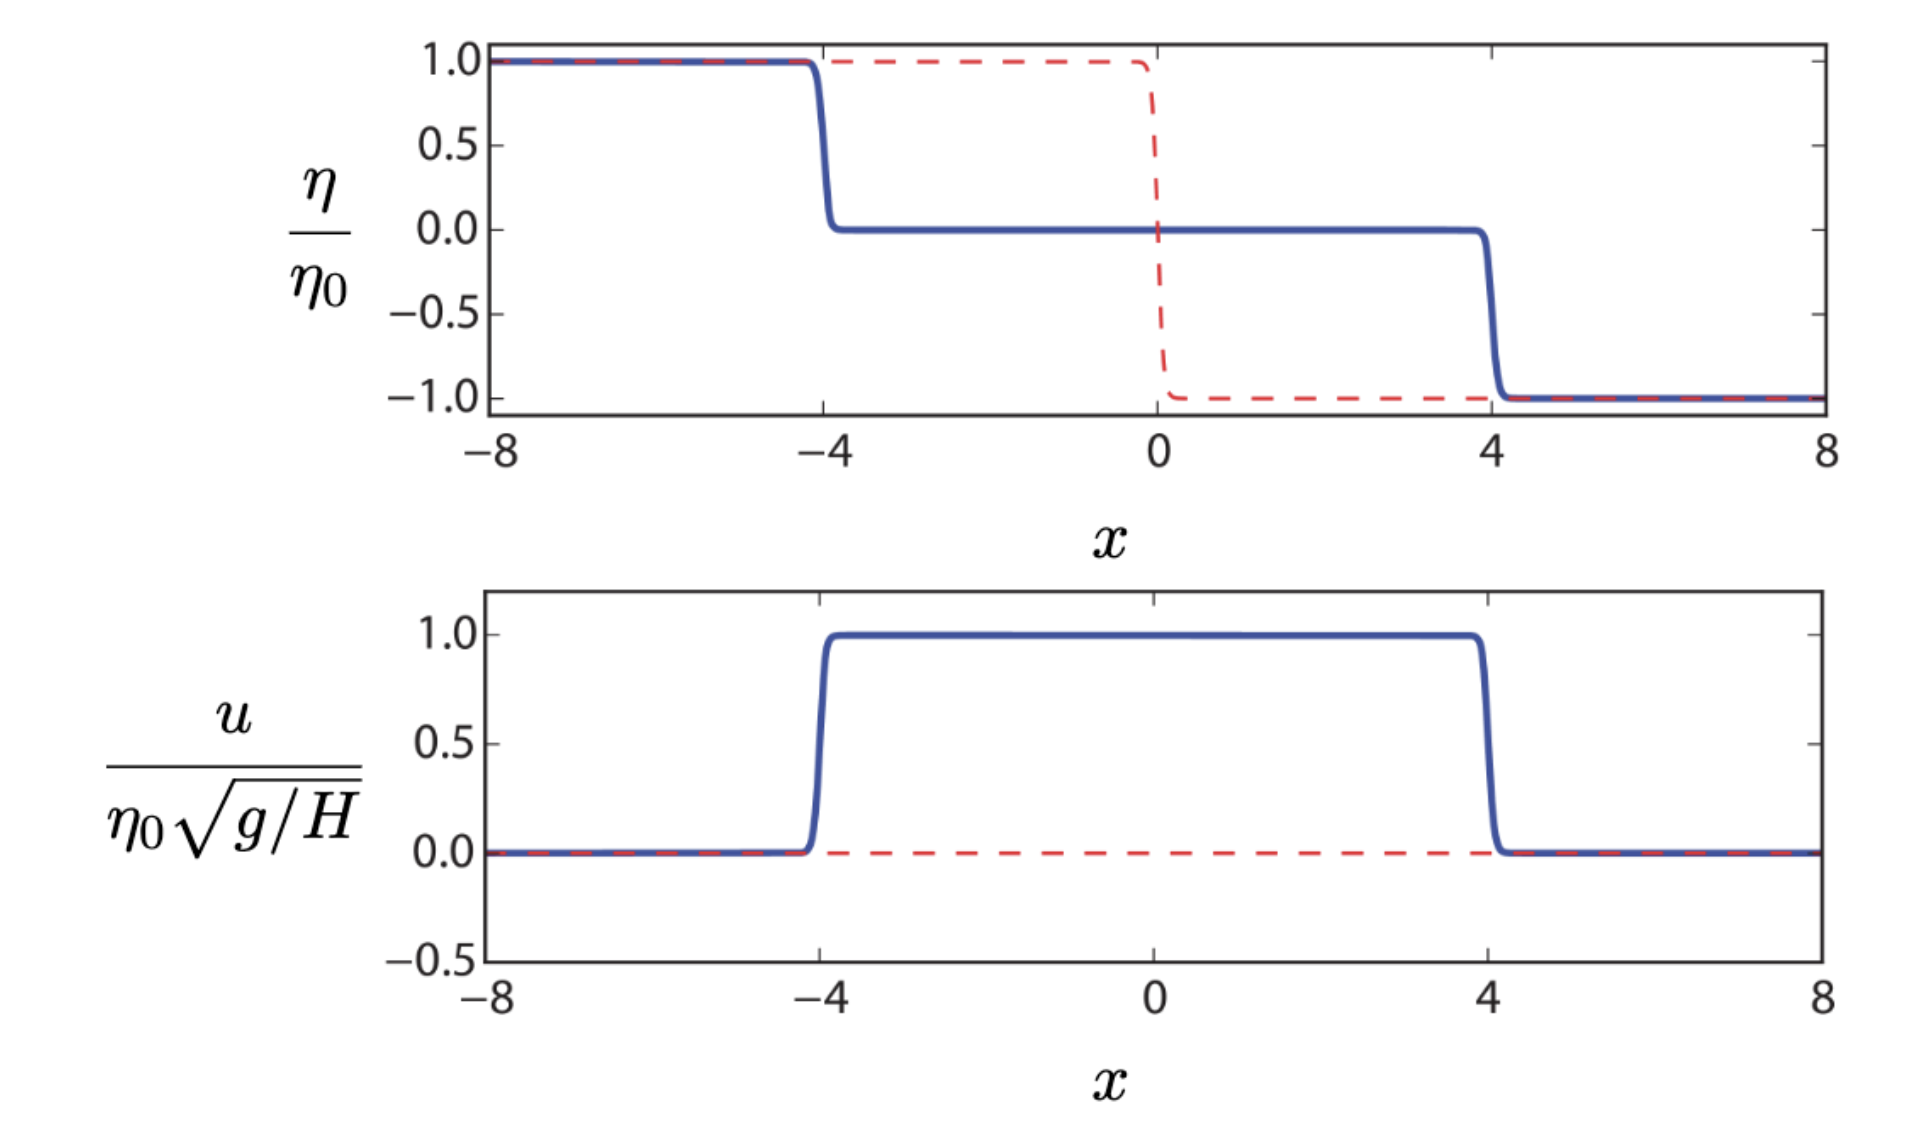
\includegraphics[width=0.8\textwidth,height=\textheight]{figures/dambreak_solution.png}

}

\caption{\label{fig-damBreakSol}The height (top) and velocity (bottom)
for the propagating height disturbance in shallow water system. The
variables are normalised. The dashed line shows the initial condition
and the solid line the solution at \(t=4/c\).}

\end{figure}

\end{tcolorbox}

\hypertarget{vortices-on-sloping-beaches}{%
\section{Vortices on sloping
beaches}\label{vortices-on-sloping-beaches}}

There are cases where the changes in \(\eta\) are small compared to the
flow and bottom surface, but the surface pressure is no longer constant.
In such cases, we need to modify the shallow water equations by changing
the top boundary condition from constant pressure to constant \(\eta\).
This boundary condition is known as a \emph{rigid lid} as it is
literally the equivalent of putting a rigid lid on the top. Using this
condition, Equation~\ref{eq-integrated_pressure} changes to
\[    p(x,y,z,t) - p(x,y,0,t) = \rho_0 g (0 - z), \] where we place our
\(z\) axis at the top surface that is nearly constant. Taking the
horizontal gradient of this equation gives,
\[  \gradH \ p(x,y,z,t)  = \gradH \ (p_0(x,y,t) =p(x,y,0,t)), \] where
we used \(p_0\) to denote the surface pressure. Note the constant
\(\eta\) assumption means that \(h(x,y,t) = - \eta_b(x,y)\). As a
result, if the bottom surface doesn't change with time (reasonable
assumption for many problems with a solid boundary),
\(\partial h /\partial t =0\). Using these assumptions, we can write the
rigid-lid shallow water equations as
\begin{equation}\protect\hypertarget{eq-riglid_SWeqs1}{}{ \frac{D \vb}{D t}  =  - \frac{1}{\rho_0}\ \gradH p_0, }\label{eq-riglid_SWeqs1}\end{equation}
\begin{equation}\protect\hypertarget{eq-riglid_SWeqs2}{}{ \gradH \cdot (h \vb) = 0, }\label{eq-riglid_SWeqs2}\end{equation}
\begin{equation}\protect\hypertarget{eq-riglid_SWeqs3}{}{ h(x,y,t) = \eta_b(x,y,t).}\label{eq-riglid_SWeqs3}\end{equation}

\begin{tcolorbox}[enhanced jigsaw, toprule=.15mm, left=2mm, opacityback=0, breakable, arc=.35mm, colback=white, rightrule=.15mm, bottomrule=.15mm, colframe=quarto-callout-note-color-frame, leftrule=.75mm]
\begin{minipage}[t]{5.5mm}
\textcolor{quarto-callout-note-color}{\faInfo}
\end{minipage}%
\begin{minipage}[t]{\textwidth - 5.5mm}

The rigid-lid shallow water system is a good approximation for flows on
sloping beaches as surface variations compared to the changes of the
bottom slope and velocities are negligible. This is also a good model
for lab experiments where the flow is confined by a solid wall from the
top.

\end{minipage}%
\end{tcolorbox}

We can transform equations
(\ref{eq-riglid_SWeqs1})-(\ref{eq-riglid_SWeqs3}) into the following
equation (see the assignment for derivation)
\begin{equation}\protect\hypertarget{eq-PV4riglidSW}{}{q = \frac{\nabla \times \vb}{h} = \frac{\partial v/\partial x - \partial u/\partial y}{h}, \quad  \frac{D q}{D t} = 0. }\label{eq-PV4riglidSW}\end{equation}

This shows that the quantity \(q\) is conserved materially (i.e.~on
particle trajectories), which has important consequences for the
dynamics. For example, if a vortex is pushed up toward shallower parts
of a sloping beach, it becomes stronger and rotates faster.

\begin{tcolorbox}[enhanced jigsaw, toprule=.15mm, left=2mm, opacityback=0, breakable, arc=.35mm, colback=white, rightrule=.15mm, bottomrule=.15mm, colframe=quarto-callout-note-color-frame, leftrule=.75mm]
\begin{minipage}[t]{5.5mm}
\textcolor{quarto-callout-note-color}{\faInfo}
\end{minipage}%
\begin{minipage}[t]{\textwidth - 5.5mm}

\(q\) as defined in Equation~\ref{eq-PV4riglidSW} is a special case of a
quantity known as Potential Vorticity (PV). We will introduce the
general form of this quantity in chapter 5 and show that is it conserved
for some limits of the shallow water and Boussinesq equations. Such a
conservation law is an important element of large-scale atmospheric and
oceanic flows.

\end{minipage}%
\end{tcolorbox}

\hypertarget{sec-chap:rotation}{%
\chapter{Rotating fluids}\label{sec-chap:rotation}}

Newton's second law applies in an inertial (non-accelerating) frame of
reference but the Earth rotates (i.e., it is not an inertial frame of
reference). Considering that we observe and measure everything from
Earth's surface, it is useful to describe flows relative to Earth's
surface rather than some inertial frame and therefore we need to recast
our governing equations into a form appropriate for a rotating frame of
reference.

\hypertarget{rotating-reference-frame}{%
\section{Rotating reference frame}\label{rotating-reference-frame}}

Consider an inertial frame of reference \(\mathrm{I}\), described by
orthogonal basis vectors \(\eb_1\), \(\eb_2\) and \(\eb_3\) and a second
frame of reference \(\mathrm{R}\) described by orthogonal basis vectors
\(\hat\eb_1\), \(\hat\eb_2\) and \(\hat\eb_3\) which is rotating with
angular velocity \(\Omb\) relative to \(\mathrm{I}\). If we define
\(\left(\ddt{}\right)_\mathrm{I}\) to be a derivative with respective to
time in the inertial frame, then clearly we have that
\(\left(\ddt{\eb_j}\right)_\mathrm{I}=0\) but
\(\left(\ddt{\hat\eb_j}\right)_\mathrm{I}\neq0\) because \(\hat\eb_j\)
is rotating relative to our inertial frame.

Now, consider a vector \(\Cb\) of constant length that is rotating
relative to the inertial frame at a constant angular velocity \(\Omb\).
It follows that, in the rotating frame \(R\), \(\Cb\) appears
stationary, i.e., \(\left(\ddt{\Cb}\right)_\mathrm{R}=0\) where now
\(\left(\ddt{}\right)_\mathrm{R}\) is a derivative taken in the rotating
frame of reference. We want to know how this vector appear to change in
time if observed from the inertial frame, i.e., what is
\(\left(\ddt{\Cb}\right)_\mathrm{I}\)?

Consider a small interval of time \(\delta t\) over which \(\Cb\)
rotates through a small angle \(\delta \lambda\) (see
Figure~\ref{fig-rotframe}). Then, the change in \(\Cb\) as observed in
the inertial frame is
\[ \delta\Cb = |\Cb|\sin\gamma\delta\lambda \eb_n \] where \(\gamma\) is
the angle between \(\Omb\) and \(\Cb\), and \(\hat n\) is the unit
vector in the direction of the change of \(\Cb\) (perpendicular to both
\(\Omb\) and \(\Cb\)). But the change in \(\lambda\) is easily obtained
from the angular velocity, in particular we have
\(\delta \lambda = |\Omb|\delta t\) and hence
\[ \delta \Cb = |\Cb||\Omb|\sin\gamma\delta t \eb_n = \Omb \times \Cb \delta t. \]
It follows that
\begin{equation}\protect\hypertarget{eq-RtoI}{}{ \left( \ddt{\Cb}\right)_\mathrm{I} = \Omb\times\Cb. }\label{eq-RtoI}\end{equation}

\begin{figure}

{\centering 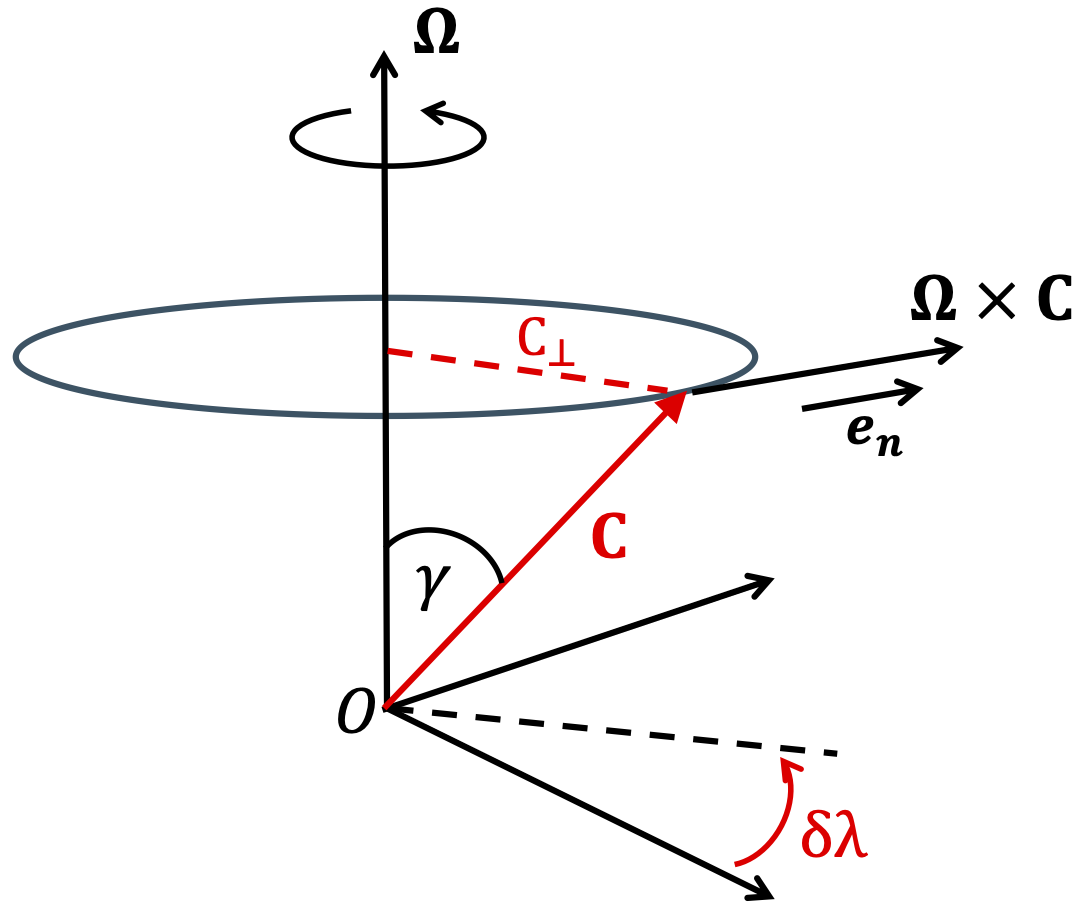
\includegraphics[width=0.5\textwidth,height=\textheight]{figures/Rotframe.png}

}

\caption{\label{fig-rotframe}A vector \(\Cb\) rotating relative to the
inertial frame at a constant angular velocity \(\Omb\). Over a small
interval of time \(\delta t\), \(\Cb\) rotates through a small angle
\(\delta \lambda\). \(\gamma\) is the angle between \(\Omb\) and
\(\Cb\), and \(\eb_n\) is the unit vector in the direction of the change
of \(\Cb\) (perpendicular to both \(\Omb\) and \(\Cb\)). Figure adapted
from Vallis.}

\end{figure}

\begin{tcolorbox}[enhanced jigsaw, left=2mm, opacityback=0, coltitle=black, bottomtitle=1mm, title={Example}, toprule=.15mm, colbacktitle=quarto-callout-tip-color!10!white, breakable, arc=.35mm, titlerule=0mm, colback=white, toptitle=1mm, opacitybacktitle=0.6, rightrule=.15mm, bottomrule=.15mm, colframe=quarto-callout-tip-color-frame, leftrule=.75mm]

Consider the case where the rotating frame is rotating about the
\(\eb_3\) axis at a constant rate \(\mathrm{\Omega}\). In this case
basis vectors for the inertial frame and the rotating frame are related
by \begin{align*}
\hat\eb_1 &= \cos(\Omrm t)\eb_1 + \sin(\Omrm t)\eb_2, \quad \hat\eb_2 = -\sin(\Omrm t)\eb_1 + \cos(\Omrm t)\eb_2, \quad \hat\eb_3 = \eb_3,\\
\eb_1 &= \cos(\Omrm t)\hat\eb_1 - \sin(\Omrm t)\hat\eb_2, \quad \eb_2 = \sin(\Omrm t)\hat\eb_1 + \cos(\Omrm t)\hat\eb_2, \quad\quad \eb_3 = \hat\eb_3.
\end{align*} Now, any vector \(\ab\) can be expressed as \begin{align*}
\ab = a_j\eb_j &= a_1(\cos(\Omrm t)\hat\eb_1 - \sin(\Omrm t)\hat\eb_2) + a_2(\sin(\Omrm t)\hat\eb_1 + \cos(\Omrm t)\hat\eb_2) + a_3\hat\eb_3\\
& = (a_1\cos(\Omrm t) + a_2\sin(\Omrm t))\hat \eb_1 + (-a_1\sin(\Omrm t) + a_2\cos(\Omrm t))\hat \eb_2 + a_3\hat\eb_3 = \hat a_j \hat\eb_j,
\end{align*} where \(\hat a_1 = a_1\cos(\Omrm t) + a_2\sin(\Omrm t)\),
\(\hat a_2 = -a_1\sin(\Omrm t) + a_2\cos(\Omrm t)\) and
\(\hat a_3=a_3\). Note the coordinates \(a_j\) and \(\hat a_j\) are
different but vector is the same.

We see that even simple trajectories can appear non-trivial in a
rotating frame, e.g.,

\begin{itemize}
\tightlist
\item
  A stationary particle with position \(\ab=(a_0,0,0)\) corresponds to
  \(\hat\ab=(a_0\cos(\Omrm t), -a_0\sin(\Omrm t),0)\) in the rotating
  frame. This is a clockwise rotation with angular velocity \(\Omrm\).
\item
  A particle moving in a straight line at speed \(v\) with position
  \(\ab=(vt,0,0)\) in the inertial frame corresponds to
  \(\hat\ab=(vt\cos(\Omrm t), -vt\sin(\Omrm t),0)\) in the rotating
  frame. This corresponds to a clockwise spiral.
\end{itemize}

Note that \begin{align*}
\left(\ddt{\hat\eb_1} \right)_\mathrm{I} &= \ddt{}(\cos(\Omrm t)\eb_1 + \sin(\Omrm t)\eb_2) = -\Omrm\sin(\Omrm t)\eb_1 + \Omrm\cos(\Omrm t)\eb_2 = \Omrm\hat\eb_2\\
\left(\ddt{\hat\eb_2} \right)_\mathrm{I} &= \ddt{}(-\sin(\Omrm t)\eb_1 + \cos(\Omrm t)\eb_2) = -\Omrm\cos(\Omrm t)\eb_1 - \Omrm\sin(\Omrm t)\eb_2 = -\Omrm\hat\eb_1\\
\left(\ddt{\hat\eb_3} \right)_\mathrm{I} &= 0.
\end{align*} Combining together, we can write
\[ \left( \ddt{\hat\eb_j}\right)_\mathrm{I} = \Omb\times\hat\eb_j \]
which is expected from Equation~\ref{eq-RtoI}.

\end{tcolorbox}

Now let's consider a general vector \(\Bb(t)=B_j(t){\hat\eb}_j\). In the
rotating frame we have that
\[ \left( \ddt{\Bb}\right)_\mathrm{R} = \ddt{}(B_j{\hat\eb}_j)_\mathrm{R} = \ddt{B_j}{\hat\eb}_j \]
since the \({\hat\eb}_j\) are stationary in the rotating frame. Note,
there is no need to state which reference frame we differentiate the
\(B_j\) in since they are scalar functions.

In the inertial frame we have \begin{align*}
\left( \ddt{\Bb}\right)_\mathrm{I} = \ddt{}(B_j{\hat\eb}_j)_\mathrm{I} &=  \ddt{B_j}{\hat\eb}_j + B_j\left(\ddt{\hat\eb_j}\right)_\mathrm{I}\\
& =  \left(\ddt{\Bb}\right)_\mathrm{R} + B_j\Omb\times\hat{\eb}_j\\
& =  \left(\ddt{\Bb}\right)_\mathrm{R} + \Omb\times(B_j\hat{\eb}_j)\\
& =  \left(\ddt{\Bb}\right)_\mathrm{R}  + \Omb\times\Bb.
\end{align*} So, for any vector \(\Bb\), we have
\begin{equation}\protect\hypertarget{eq-rotframeref}{}{\left( \ddt{\Bb}\right)_\mathrm{I} =  \left(\ddt{\Bb}\right)_\mathrm{R}  + \Omb\times\Bb. }\label{eq-rotframeref}\end{equation}

\hypertarget{dynamics-in-a-rotating-frame}{%
\section{Dynamics in a rotating
frame}\label{dynamics-in-a-rotating-frame}}

If we take \(\Bb=\Xb\) in Equation~\ref{eq-rotframeref} to be the
position vector of a fluid parcel, then we have that
\[ \ub_\mathrm{I} = \ub_\mathrm{R} +  \Omb\times\Xb \] where
\(\ub_\mathrm{I}\) is the perceived velocity in the inertial frame, and
\(\ub_\mathrm{R}\) is the perceived velocity in the rotating frame.

Then, to consider how accelerations are viewed in a rotating frame, put
\(\Bb=\ub_\mathrm{I}\) in Equation~\ref{eq-rotframeref}: \begin{align*}
\left( \ddt{\ub}\right)_\mathrm{I} & =  \left(\ddt{\ub}\right)_\mathrm{R}  + \Omb\times\ub_\mathrm{I}\\
& = \left(\ddt{}(\ub_\mathrm{R}+  \Omb\times\Xb)\right)_\mathrm{R} + \Omb\times(\ub_\mathrm{R}+  \Omb\times\Xb)\\
& = \left(\ddt{\ub}\right)_\mathrm{R}+  \Omb\times\left(\ddt{\Xb}\right)_\mathrm{R} + \Omb\times\ub_\mathrm{R}+ \Omb\times(\Omb\times\Xb)\\
& = \left(\ddt{\ub}\right)_\mathrm{R}+  2\Omb\times\ub_\mathrm{R} + \Omb\times(\Omb\times\Xb).
\end{align*} In an inertial frame Newton's law gives (for a fluid parcel
of mass \(m\)) \[
\left( \ddt{\ub}\right)_\mathrm{I} = \frac{1}{m}\Fb,
\] so when viewed in a rotating frame, the same parcel obeys \[
\left( \ddt{\ub}\right)_\mathrm{R} = \frac{1}{m}\Fb - 2\Omb\times\ub_\mathrm{R} - \Omb\times(\Omb\times\Xb).
\]

The extra ``force'' terms that appear on the right-hand-side are a
result of working in a non-inertial reference frame. Since the forces
are not real, they are often referred to as \emph{fictitious} or
\emph{apparent} forces. The second term on the right-hand-side is known
as the \textbf{Coriolis force}. If \(\Omb\) points up (down), the
Coriolis force deflects horizontally moving objects to the right (left)
when observed in a rotating frame of reference.

The third term on the right-hand-side is known as the
\textbf{Centrifugal force}. This force appears to push objects away from
the rotation axis.

Now that we can treat accelerations appropriately, we can write down the
momentum equation in a rotating frame of reference. We just need to
replace \(\DDt{\ub_\mathrm{I}}\) with
\begin{equation}\protect\hypertarget{eq-transformtorotframe}{}{
\DDt{\ub_\mathrm{R}} + 2\Omb \times\ub_\mathrm{R} + \Omb\times(\Omb \times \Xb).
}\label{eq-transformtorotframe}\end{equation} For example, in the case
of the Boussinesq equations, the momentum equation (\ref{eq-Bousmom})
becomes \[
\DDt{\ub_\mathrm{R}}  +2\Omb\times\ub_\mathrm{R} +\Omb\times(\Omb \times \Xb) = -\frac{1}{\bar\rho}\nabla p +b\eb_z.
\]

As density (or buoyancy) is a scalar, Equation~\ref{eq-Bousdenistybuoy}
is unchanged in a rotating frame and therefore the Boussinesq equations
in a rotating frame can be summarised as:

\begin{equation}\protect\hypertarget{eq-Bousmomrot}{}{ \DDt{\ub}  + 2\Omb\times\ub +\Omb\times(\Omb \times \Xb) = -\frac{1}{\bar\rho}\nabla p +b\eb_z, }\label{eq-Bousmomrot}\end{equation}
\begin{equation}\protect\hypertarget{eq-Bousdivu0rot}{}{  \nabla\cdot\ub = 0,}\label{eq-Bousdivu0rot}\end{equation}
\begin{equation}\protect\hypertarget{eq-Bousdensityrot}{}{ \DDt{b} +N^2(z)w=0,}\label{eq-Bousdensityrot}\end{equation}
where we have dropped the subscript \(\mathrm{R}\) from the velocity as
we simply interpret \(\ub\) in these equations to be the velocity in a
rotating frame of reference.

\begin{tcolorbox}[enhanced jigsaw, toprule=.15mm, left=2mm, opacityback=0, breakable, arc=.35mm, colback=white, rightrule=.15mm, bottomrule=.15mm, colframe=quarto-callout-note-color-frame, leftrule=.75mm]
\begin{minipage}[t]{5.5mm}
\textcolor{quarto-callout-note-color}{\faInfo}
\end{minipage}%
\begin{minipage}[t]{\textwidth - 5.5mm}

Here we have allowed for the effects of rotation by writing the
(non-hydrostatic) Boussinesq momentum equation in a rotating reference
frame. Note that other equation sets (e.g., the the shallow water,
incompressible Navier-Stokes and hydrostatic Boussinesq equations) can
be written in a rotating frame of reference in a similar way, i.e., by
using Equation~\ref{eq-transformtorotframe} to incorporate the Coriolis
and centrifugal forces in the momentum equations. We will make use of
this in future sections.

\end{minipage}%
\end{tcolorbox}

\hypertarget{sec-centrifugalpotential}{%
\subsection{Centrifugal force as a
potential}\label{sec-centrifugalpotential}}

A simplification to these equations can be made if we are able to write
the centrifugal force as the gradient of a scalar potential that can
then be combined with the pressure. To do this, we define a set of
cylindrical polar coordinates \((s,\theta,z)\) in which the \(z\)-axis
is aligned with the rotation axis, i.e., with \(\Omb\). \(s\) is then
the perpendicular distance from the \(z\)-axis. Since in cylindrical
polars, the position vector is given by \(\Xb = s\eb_s+z\eb_z\) we have
that \[
\Omb\times(\Omb\times\Xb) = \Omrm\eb_z \times \Omrm s \eb_\theta = -\Omrm^2 s \eb_s,
\] demonstrating that the centrifugal force
\(-\Omb\times(\Omb\times\Xb)\) pushes objects away from the rotation
axis. Now, we want to find a potential \(\phi_c\) such that
\(\nabla \phi_c = \Omb\times(\Omb\times\Xb)\). It follows that \[
\frac{\partial \phi_c}{\partial s} = -\Omrm^2s, \quad \quad \frac{\partial \phi_c}{\partial \theta} = \frac{\partial \phi_c}{\partial z} = 0,
\] and hence
\(\phi_c = -\frac{\Omrm^2s^2}{2} = -\frac{1}{2}|\Omb \times \Xb|^2\).

Writing the centrifugal force as
\(-\Omb\times(\Omb\times\Xb) = -\nabla \phi_c\) allows us to simplify
Equation~\ref{eq-Bousmomrot} to give
\begin{equation}\protect\hypertarget{eq-Bousmomrotpot}{}{  \DDt{\ub}  +2\Omb\times\ub  = -\frac{1}{\bar\rho}\nabla p_r + b \eb_z,}\label{eq-Bousmomrotpot}\end{equation}
where \(p_r = p + \bar\rho\phi_c\).

\begin{tcolorbox}[enhanced jigsaw, toprule=.15mm, left=2mm, opacityback=0, breakable, arc=.35mm, colback=white, rightrule=.15mm, bottomrule=.15mm, colframe=quarto-callout-note-color-frame, leftrule=.75mm]
\begin{minipage}[t]{5.5mm}
\textcolor{quarto-callout-note-color}{\faInfo}
\end{minipage}%
\begin{minipage}[t]{\textwidth - 5.5mm}

To simplify the notation we drop the subscript \(r\) in the rest of this
course, while we consider the modified pressure that includes the
centrifugal effect.

\end{minipage}%
\end{tcolorbox}

\begin{tcolorbox}[enhanced jigsaw, toprule=.15mm, left=2mm, opacityback=0, breakable, arc=.35mm, colback=white, rightrule=.15mm, bottomrule=.15mm, colframe=quarto-callout-note-color-frame, leftrule=.75mm]
\begin{minipage}[t]{5.5mm}
\textcolor{quarto-callout-note-color}{\faInfo}
\end{minipage}%
\begin{minipage}[t]{\textwidth - 5.5mm}

Similar to centrifugal force, gravity can be formulated as a potential
\(\phi_g\) such that \(\gb=-\nabla \phi_g\). Taking the Earth to be a
perfect sphere of radius \(r_e = 6371\mathrm{km}\) and mass
\(M=5.98\times10^{24}\mathrm{kg}\), Newton's law of gravitation gives
\(\phi_g = -GM/r\) where
\(G=6.67\times10^{-11}\mathrm{m^3kg^{-1}s^{-2}}\) is the gravitational
constant. Then \(\gb=\nabla(GM/r)=-(GmM/r^2)\eb_r\) (points radially
inwards). At the Earth's surface
\(|\gb|=GM/r_e^2=9.82\mathrm{ms^{-2}}\). If the height (depth) changes
are small enough, we can assume that \(\gb\) is locally constant, which
is what we consider for the rest of this course. However, if in an
application dynamics takes place in a thick layer of fluid, the
variation of \(\gb\) should be properly taken into account.

\end{minipage}%
\end{tcolorbox}

\hypertarget{sec-tang_plane_approx}{%
\section{Tangent-plane approximation}\label{sec-tang_plane_approx}}

To study the fluid dynamics of oceans and atmospheres, it is convenient
to work in a frame of reference rotating with the planet. In this
course, our model planet will be the Earth. The spherical geometry of
Earth can influence the dynamics of flows and make studying them more
involved. However, the sphericity of the Earth is not always as
important as its rotation. In this case, it is more convenient to use a
locally Cartesian model and introduce two approximations.

In spherical polar coordinates \((r,\theta,\phi)\) where \(r\) is a
radial coordinate, \(\theta\) is the latitude (angle measured northwards
from the equator) and \(\phi\) is the longitutde we have that
\begin{equation}
\Omb = \Omrm\sin\theta\eb_r + \Omrm\cos\theta \eb_\theta.
\end{equation} That is, \(\Omb\) in its most general form has a radially
(locally vertical) and a meridional (locally horizontal) component which
both depend on latitude \(\theta\). However, if we limit the dynamics to
a region where the changes in \(\theta\) are small, we can make a set of
simplifications. We define a plane tangent to the surface of the Earth
at a latitude \(\theta_0\) and use a Cartesian system to define the
motion (see figure \ref{fig:Tangent_plane}). We take the \(z\)-axis to
point in the direction of \(-\nabla\Phi\) and write
\(-\nabla\Phi=g\eb_z\) where \(g\) is taken to be constant over the
depth of the (thin) layer. \(x\) is taken to point eastwards and \(y\)
northwards. We define \(y=0\) at \(\theta=\theta_0\).

\begin{figure}

{\centering 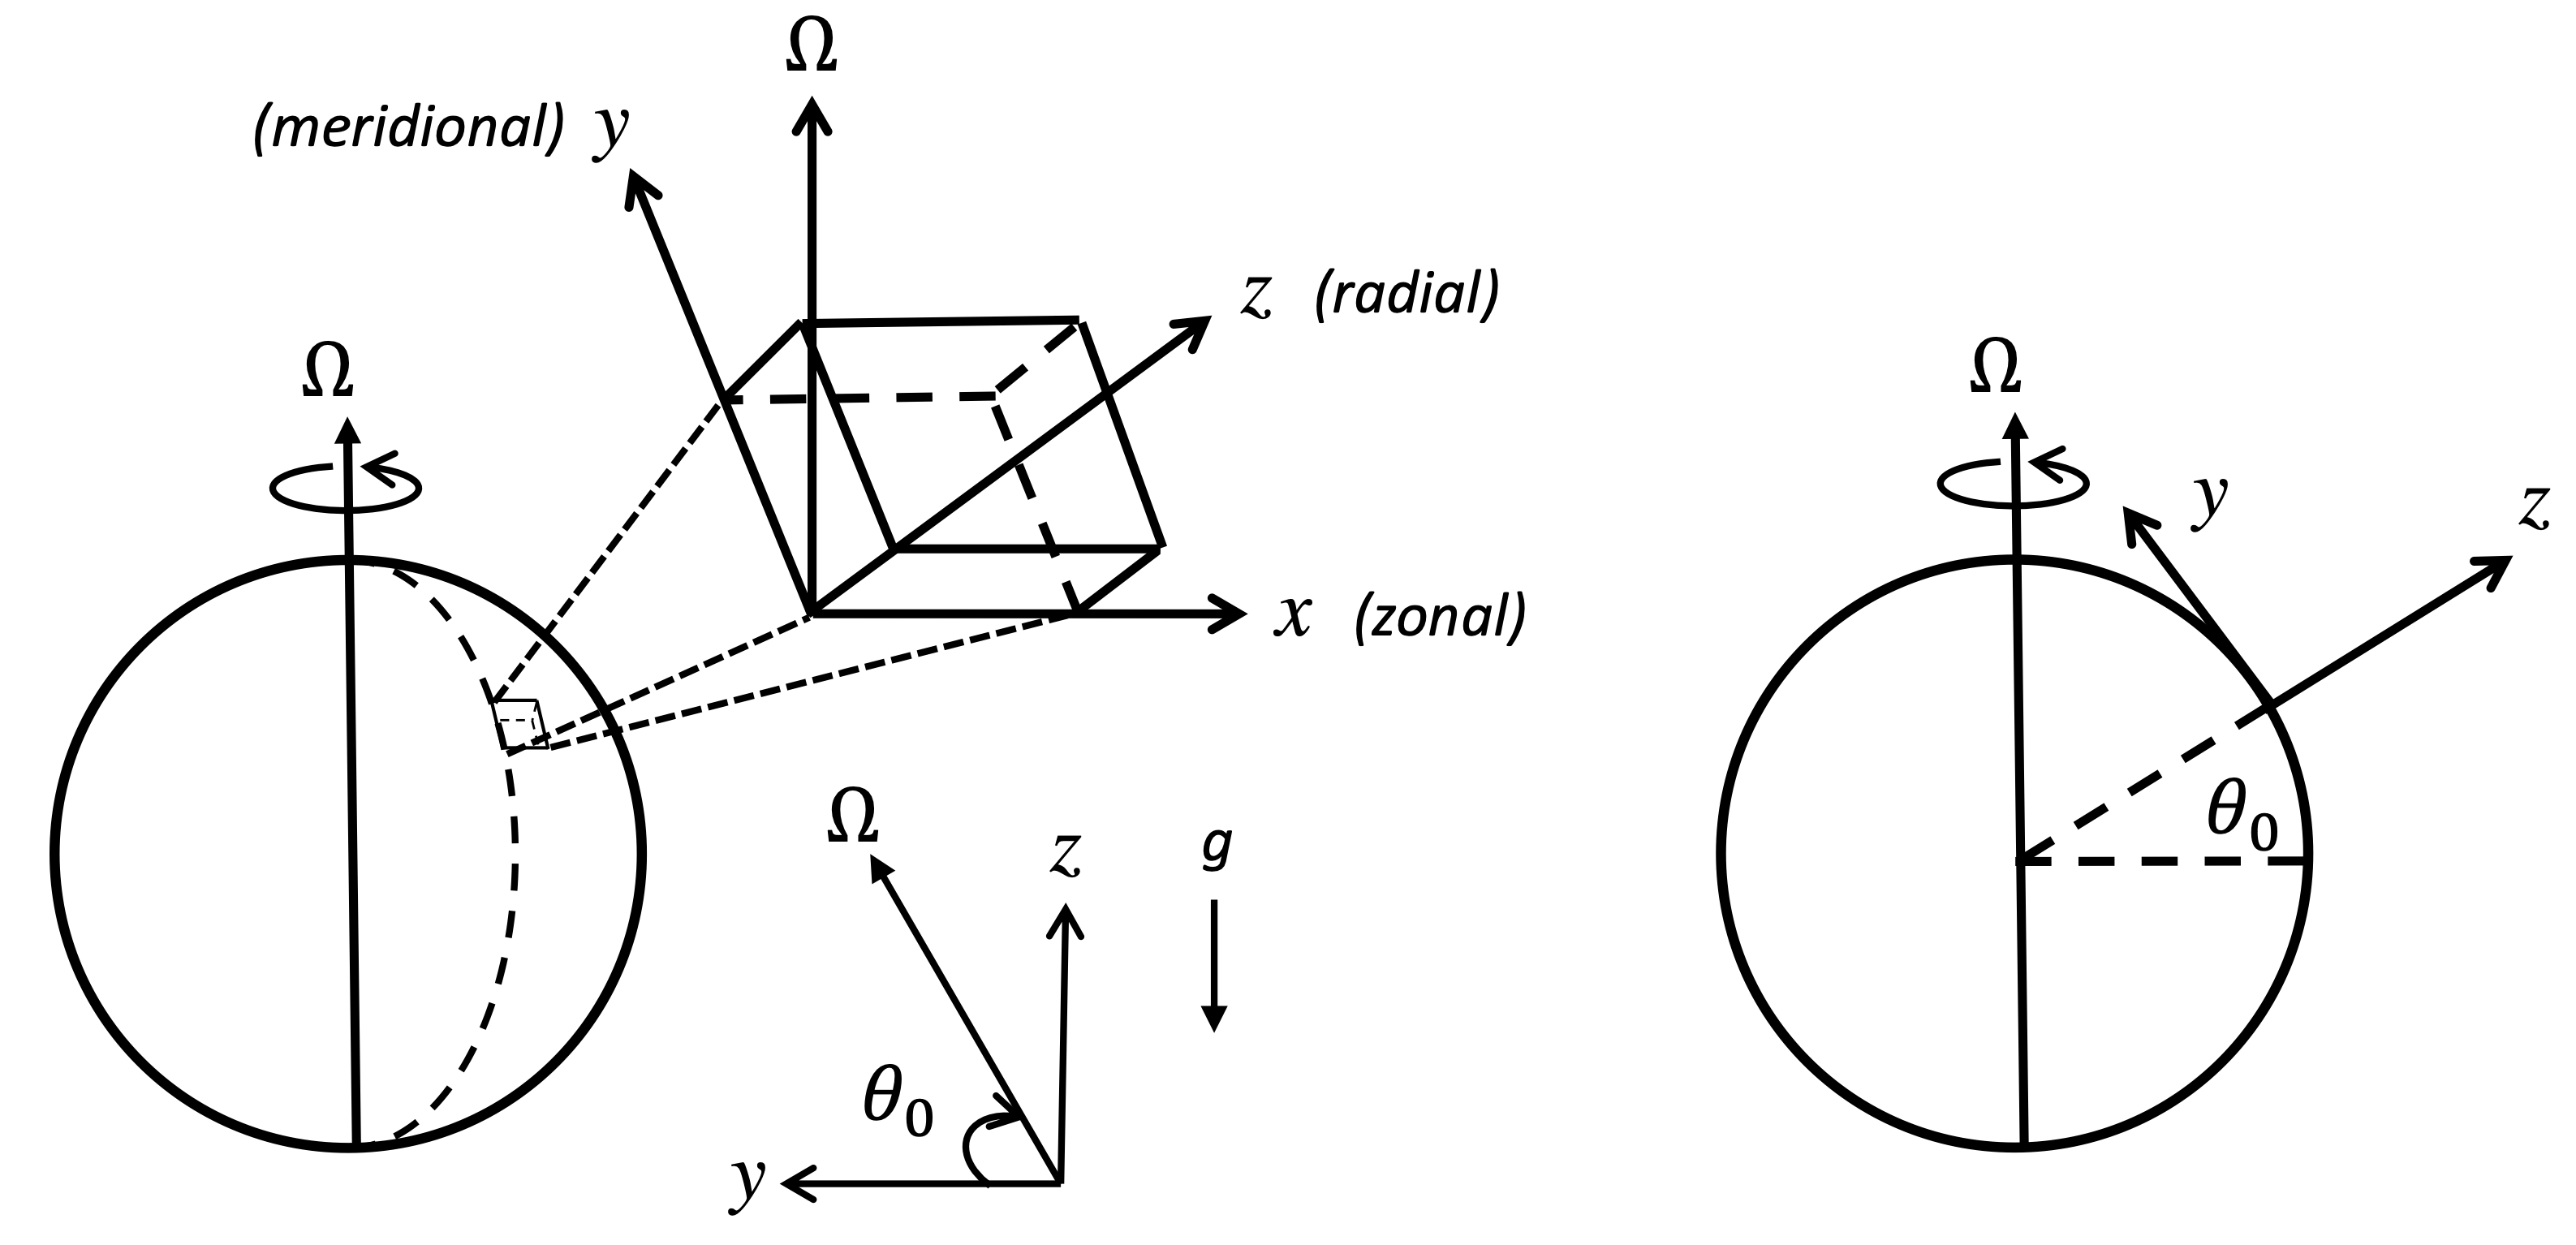
\includegraphics[width=0.9\textwidth,height=\textheight]{figures/Tangent_plane.png}

}

\caption{\label{fig-Tangent_plane}Tangent plane approximation.}

\end{figure}

Since the geopotential force is directed almost radially inwards, we
take \(\eb_r\approx\eb_z\) and \(\eb_\theta\approx\eb_y\) at
\(\theta=\theta_0\) and we make the approximation \[
\Omb=\Omrm\sin\theta\eb_r+\Omrm\cos\theta\eb_\theta \approx \Omrm\sin\theta\eb_z+\Omrm\cos\theta\eb_y.
\] For small \(\theta-\theta_0\), \(y\approx r_e(\theta-\theta_0)\) and
so we have that \begin{align*}
\sin\theta&=\sin(\theta+(\theta-\theta_0)) =\sin\theta_0 + (\theta-\theta_0)\cos\theta_0 + O((\theta-\theta_0)^2) \approx \sin\theta_0 +\frac{\cos\theta_0}{r_e}y\\
\cos\theta&=\cos(\theta+(\theta-\theta_0)) = \cos\theta_0 - (\theta-\theta_0)\sin\theta_0 + O((\theta-\theta_0)^2) \approx \cos\theta_0 -\frac{\sin\theta_0}{r_e}y.
\end{align*} Hence we write \(\Omb = \Omrm_z\eb_z + \Omrm_y\eb_y\) where
\begin{align*}
\Omrm_z&=\Omrm\sin\theta_0+\frac{\Omrm\cos\theta_0}{r_e}y\\
\Omrm_y&=\Omrm\cos\theta_0-\frac{\Omrm\sin\theta_0}{r_e}y.
\end{align*}

The Coriolis force \(2\Omb\times \ub\) can then be written as \[
2\Omb\times \ub = (2\Omrm_y w - 2\Omrm_z v, 2\Omrm_z u, -2\Omrm_y u)
\] Hence the Cartesian components of momentum equations under the
tangent plane approximation are:
\begin{equation}\protect\hypertarget{eq-tangentplaneu}{}{ \DDt{u} + 2(\Omrm_yw-\Omrm_zv) = -\frac{1}{\rho}\frac{\partial p}{\partial x} }\label{eq-tangentplaneu}\end{equation}
\begin{equation}\protect\hypertarget{eq-tangentplanev}{}{ \DDt{v} + 2\Omrm_z u = -\frac{1}{\rho}\frac{\partial p}{\partial y} }\label{eq-tangentplanev}\end{equation}
\begin{equation}\protect\hypertarget{eq-tangentplanew}{}{\DDt{w}  -2\Omrm_y u = -\frac{1}{\rho}\frac{\partial p}{\partial z} -g. }\label{eq-tangentplanew}\end{equation}

If we further assume that the layer is thin then the vertical flow speed
is much smaller than the horizontal flow speeds, i.e.,
\(|w| \ll |u| \text{ and } |v|\). We can therefore drop the
\(\Omrm_y w\) term in Equation~\ref{eq-tangentplaneu}. Then, to ensure
energy is still conserved we must then also drop the \(-\Omrm_y u\) term
from Equation~\ref{eq-tangentplanew} although in someways this is less
physically justified. This leads to the following set of equations:
\begin{align}
\DDt{u} -fv &= -\frac{1}{\rho}\frac{\partial p}{\partial x} \\
\DDt{v} + fu &= -\frac{1}{\rho}\frac{\partial p}{\partial y} \\
\DDt{w}   &= -\frac{1}{\rho}\frac{\partial p}{\partial z} -g,
\end{align} where we have introduced \(f=2\Omrm_z\). Equivalently, these
equations can be written in vector form as
\begin{equation}\protect\hypertarget{eq-fvecform}{}{
\DDt{\ub} + \fb\times\ub = -\frac{1}{\rho}\nabla p -g\eb_z,
}\label{eq-fvecform}\end{equation} where \(\fb=f(y)\eb_z\). This
formulation in which components of \(\Omb\) not in the direction of the
local vertical is sometimes called the \emph{traditional approximation}.
Note, the centrifugal potential no longer appears in our equations, this
is a result of defining the local vertical in the direction of
\(-\nabla\Phi\). Therefore, rotation enters the equations only through
the Coriolis force and \(f\) is often called the \emph{Coriolis
parameter}.

\(f\) is an important parameter in rotating fluid dynamics and it is
often written as \[
f = f_0 + \beta y, \quad\quad \text{where } f_0= 2\Omrm\sin\theta_0, \quad \beta = \frac{2\Omrm\cos\theta_0}{r_e}.
\] Note that \(f_0\) is positive in the northern hemisphere
(\(\theta_0>0\)), negative in the southern hemisphere (\(\theta_0<0\)),
and zero at the equator (\(\theta_0=0\)). Representing \(f\) in this way
is the basis of the so-called \textbf{\(\beta\)-plane approximation},
with the \(\beta\) term containing the latitudinal variations in \(f\).

If the flows we care about are extremely localised then we do not need
to take the latitudinal variations in \(f\) into account and we can make
a further approximation given by \(f=f_0=2\Omrm\sin\theta_0\). This is
known as the \textbf{\(f\)-plane approximation}. Note, under the
\(f\)-plane approximation (i.e., with \(f\) constant),
Equation~\ref{eq-fvecform} is analogous to that used in sections
\ref{sec-geobal} - \ref{sec-thermalwind} where we took
\(\Omb = \Omrm\eb_z\) (provided we replace \(2\Omrm\) by \(f_0\)) and so
physical concepts such as geostrophic balance, Taylor-Proudman, and
thermal wind balance are relevant on the \(f\)-plane too.

Considering the tangent plane approximation
\(2\Omb \approx \fb=f \eb_z\), we rewrite the important equations in
geophysical fluid dynamics (Boussinesq and Shallow Water) that we focus
on in this course in the rotating frame of reference.

\begin{tcolorbox}[enhanced jigsaw, left=2mm, opacityback=0, coltitle=black, bottomtitle=1mm, title={\textbf{Inviscid Shallow Water Equations}}, toprule=.15mm, colbacktitle=quarto-callout-important-color!10!white, breakable, arc=.35mm, titlerule=0mm, colback=white, toptitle=1mm, opacitybacktitle=0.6, rightrule=.15mm, bottomrule=.15mm, colframe=quarto-callout-important-color-frame, leftrule=.75mm]

\begin{equation}\protect\hypertarget{eq-rtSW1}{}{  \frac{\partial \vb}{\partial t} + (\vb\cdot\nabla)\vb   + \fb\times\vb =  - g \ \gradH \eta. }\label{eq-rtSW1}\end{equation}
\begin{equation}\protect\hypertarget{eq-rtSW2}{}{ \frac{\partial h}{\partial t} + \gradH \cdot (h \vb) = 0,  }\label{eq-rtSW2}\end{equation}
\begin{equation}\protect\hypertarget{eq-rtSW3}{}{  h(x,y,t) = \eta(x,y,t) - \eta_b(x,y,t). }\label{eq-rtSW3}\end{equation}

\end{tcolorbox}

\begin{tcolorbox}[enhanced jigsaw, left=2mm, opacityback=0, coltitle=black, bottomtitle=1mm, title={\textbf{(Hydrostatic) Boussinesq Equations}}, toprule=.15mm, colbacktitle=quarto-callout-important-color!10!white, breakable, arc=.35mm, titlerule=0mm, colback=white, toptitle=1mm, opacitybacktitle=0.6, rightrule=.15mm, bottomrule=.15mm, colframe=quarto-callout-important-color-frame, leftrule=.75mm]

\begin{equation}\protect\hypertarget{eq-rtBoussinesqHydrostat1}{}{   \frac{\partial \vb}{\partial t} + (\ub\cdot\nabla)\vb  + \fb\times\vb = -\frac{1}{\bar\rho}\gradH p,}\label{eq-rtBoussinesqHydrostat1}\end{equation}
\begin{equation}\protect\hypertarget{eq-rthydroapprox_hydrobal}{}{   \frac{\partial p}{\partial z}  = \bar\rho b = -\rho g,}\label{eq-rthydroapprox_hydrobal}\end{equation}
\begin{equation}\protect\hypertarget{eq-rtBoussinesqHydrostat3}{}{   \nabla\cdot \ub =0,}\label{eq-rtBoussinesqHydrostat3}\end{equation}
\begin{equation}\protect\hypertarget{eq-rtBoussinesqHydrostat4}{}{    \frac{\partial b}{\partial t} + (\ub\cdot\nabla)b +N^2w =0,}\label{eq-rtBoussinesqHydrostat4}\end{equation}

\end{tcolorbox}

\begin{tcolorbox}[enhanced jigsaw, left=2mm, opacityback=0, coltitle=black, bottomtitle=1mm, title={\textbf{Rotating (Non-hydrostatic) Boussinesq Equations}}, toprule=.15mm, colbacktitle=quarto-callout-important-color!10!white, breakable, arc=.35mm, titlerule=0mm, colback=white, toptitle=1mm, opacitybacktitle=0.6, rightrule=.15mm, bottomrule=.15mm, colframe=quarto-callout-important-color-frame, leftrule=.75mm]

\begin{equation}\protect\hypertarget{eq-rtBousmombuoy}{}{ \frac{\partial\ub}{\partial t} + (\ub\cdot\nabla)\ub + \fb\times\ub = -\frac{1}{\bar\rho}\nabla p +b\eb_z, }\label{eq-rtBousmombuoy}\end{equation}
\begin{equation}\protect\hypertarget{eq-rtBousdivu0buoy}{}{\nabla\cdot\ub=0,  }\label{eq-rtBousdivu0buoy}\end{equation}
\begin{equation}\protect\hypertarget{eq-rtBousdenistybuoy}{}{\frac{\partial b}{\partial t}+(\ub\cdot\nabla)b+N^2(z)w=0,}\label{eq-rtBousdenistybuoy}\end{equation}

\end{tcolorbox}

\hypertarget{rotationally-dominated-flow}{%
\section{Rotationally dominated
flow}\label{rotationally-dominated-flow}}

\hypertarget{sec-geobal}{%
\subsection{Geostrophic balance}\label{sec-geobal}}

In some fluid flows (e.g.~large-scale dynamics in the atmosphere and
ocean), the Coriolis force and pressure gradients appear to be much
larger than the other forces or acceleration terms. As a result, the
horizontal components of Equation~\ref{eq-rtBousmombuoy} (or
Equation~\ref{eq-rtBoussinesqHydrostat1}) reduce to

\begin{equation}\protect\hypertarget{eq-geobal}{}{
\fb\times\ub = -\frac{1}{\bar\rho}\gradH p.
}\label{eq-geobal}\end{equation} This equation represents an important
balance in geophysical fluid dynamics and is known as
\textbf{geostrophic balance}. It follows from Equation~\ref{eq-geobal}
that \(\ub\cdot\nabla p=0\) for the horizontal components of velocity.
Then, since surfaces of constant pressure have normal \(\nabla p\),
horizontal wind flows along lines of constant pressure.

\begin{tcolorbox}[enhanced jigsaw, toprule=.15mm, left=2mm, opacityback=0, breakable, arc=.35mm, colback=white, rightrule=.15mm, bottomrule=.15mm, colframe=quarto-callout-note-color-frame, leftrule=.75mm]
\begin{minipage}[t]{5.5mm}
\textcolor{quarto-callout-note-color}{\faInfo}
\end{minipage}%
\begin{minipage}[t]{\textwidth - 5.5mm}

We will put the concept of geophysical balance on firmer mathematical
footing in chapter 5.

\end{minipage}%
\end{tcolorbox}

\begin{tcolorbox}[enhanced jigsaw, left=2mm, opacityback=0, coltitle=black, bottomtitle=1mm, title={Example}, toprule=.15mm, colbacktitle=quarto-callout-tip-color!10!white, breakable, arc=.35mm, titlerule=0mm, colback=white, toptitle=1mm, opacitybacktitle=0.6, rightrule=.15mm, bottomrule=.15mm, colframe=quarto-callout-tip-color-frame, leftrule=.75mm]

Consider a region of atmosphere rotating about a vertical axis
(\(\Omb = \Omrm \eb_z\)) which is at higher pressure than in surrounding
regions (sometimes called a high pressure centre) so that the negative
pressure gradient \(-\nabla p\) is pointing away from the centre of the
region. The gas will want to move from high pressure to low pressure but
the gas will be pushed to the right by the Coriolis force so that it
moves in a clockwise (or \emph{anticyclonic}) motion around the high
pressure centre. In the southern hemisphere anticyclones are still
associated with regions of high pressure but in that case the motion
will be anti-clockwise.

\end{tcolorbox}

\hypertarget{taylor-proudman-theorem}{%
\subsection{Taylor-Proudman theorem}\label{taylor-proudman-theorem}}

If in the vertical direction we assume hydrostatic balance (as when
making the hydrostatic approximation in Section~\ref{sec-hydroapprox})
so that we have \begin{equation}\protect\hypertarget{eq-TPhydrobal}{}{
\frac{\partial p}{\partial z} = -\rho g,
}\label{eq-TPhydrobal}\end{equation} and if we consider the case where
density is a function of \(z\) only and the background rotation is
aligned with gravity, i.e., \(\Omb=\Omrm \eb_z\), then geostrophic
balance in the horizontal direction gives us (see
Equation~\ref{eq-geobal})
\begin{equation}\protect\hypertarget{eq-horizgeobal}{}{
-f v = -\frac{1}{\bar\rho}\frac{\partial p}{\partial x}, \quad \quad f u = -\frac{1}{\bar\rho}\frac{\partial p}{\partial y}.
}\label{eq-horizgeobal}\end{equation} These equations can be rearranged
to give \begin{equation}\protect\hypertarget{eq-geobalcomponents}{}{
 v = \frac{\partial}{\partial x}\frac{p}{f\bar\rho}, \quad \quad u = -\frac{\partial}{\partial y}\frac{p}{f\bar\rho}.
}\label{eq-geobalcomponents}\end{equation} It follows form here that
\(\frac{\partial u}{\partial x} + \frac{\partial v}{\partial y} = 0\)
and so it must be that \(\frac{\partial w}{\partial z}=0\) (from
Equation~\ref{eq-Bousdivu0rot}). In other words, the vertical velocity
is independent of height.

Now, since \(\rho=\rho(z)\), Equation~\ref{eq-TPhydrobal} gives
\(\frac{\partial^2 p}{\partial x\partial z} = \frac{\partial^2 p}{\partial y\partial z}=0\)
and so Equation~\ref{eq-geobalcomponents} then gives us that
\(\frac{\partial u}{\partial z}=\frac{\partial v}{\partial z}=0\)
(recall \(\bar\rho\) is a constant). Therefore we have that the
horizontal flow is also independent of height.

We have shown what is commonly known as the \textbf{Taylor-Proudman
theorem} which says within a fluid that is steadily rotated at high
angular velocity, the fluid velocity will be uniform along any line
parallel to the axis of rotation. For example, if there is a solid
horizontal boundary, at the surface, say, then \(w=0\) at that boundary
and so (since vertical derivatives are zero) \(w=0\) everywhere. Hence
the flow is essentially two-dimensional.

\begin{tcolorbox}[enhanced jigsaw, toprule=.15mm, left=2mm, opacityback=0, breakable, arc=.35mm, colback=white, rightrule=.15mm, bottomrule=.15mm, colframe=quarto-callout-note-color-frame, leftrule=.75mm]
\begin{minipage}[t]{5.5mm}
\textcolor{quarto-callout-note-color}{\faInfo}
\end{minipage}%
\begin{minipage}[t]{\textwidth - 5.5mm}

In reality, we do not see exact two-dimensional flow in the atmosphere
of the oceans (essentially because of stratification). However, it is
not uncommon in geophysical fluid dynamics for effects like
Taylor-Proudman to manifest in the real flow, even if assumptions
underlying a phenomena are not fully satisfied.

\end{minipage}%
\end{tcolorbox}

\begin{tcolorbox}[enhanced jigsaw, left=2mm, opacityback=0, coltitle=black, bottomtitle=1mm, title={Example}, toprule=.15mm, colbacktitle=quarto-callout-tip-color!10!white, breakable, arc=.35mm, titlerule=0mm, colback=white, toptitle=1mm, opacitybacktitle=0.6, rightrule=.15mm, bottomrule=.15mm, colframe=quarto-callout-tip-color-frame, leftrule=.75mm]

\begin{figure}[H]

{\centering 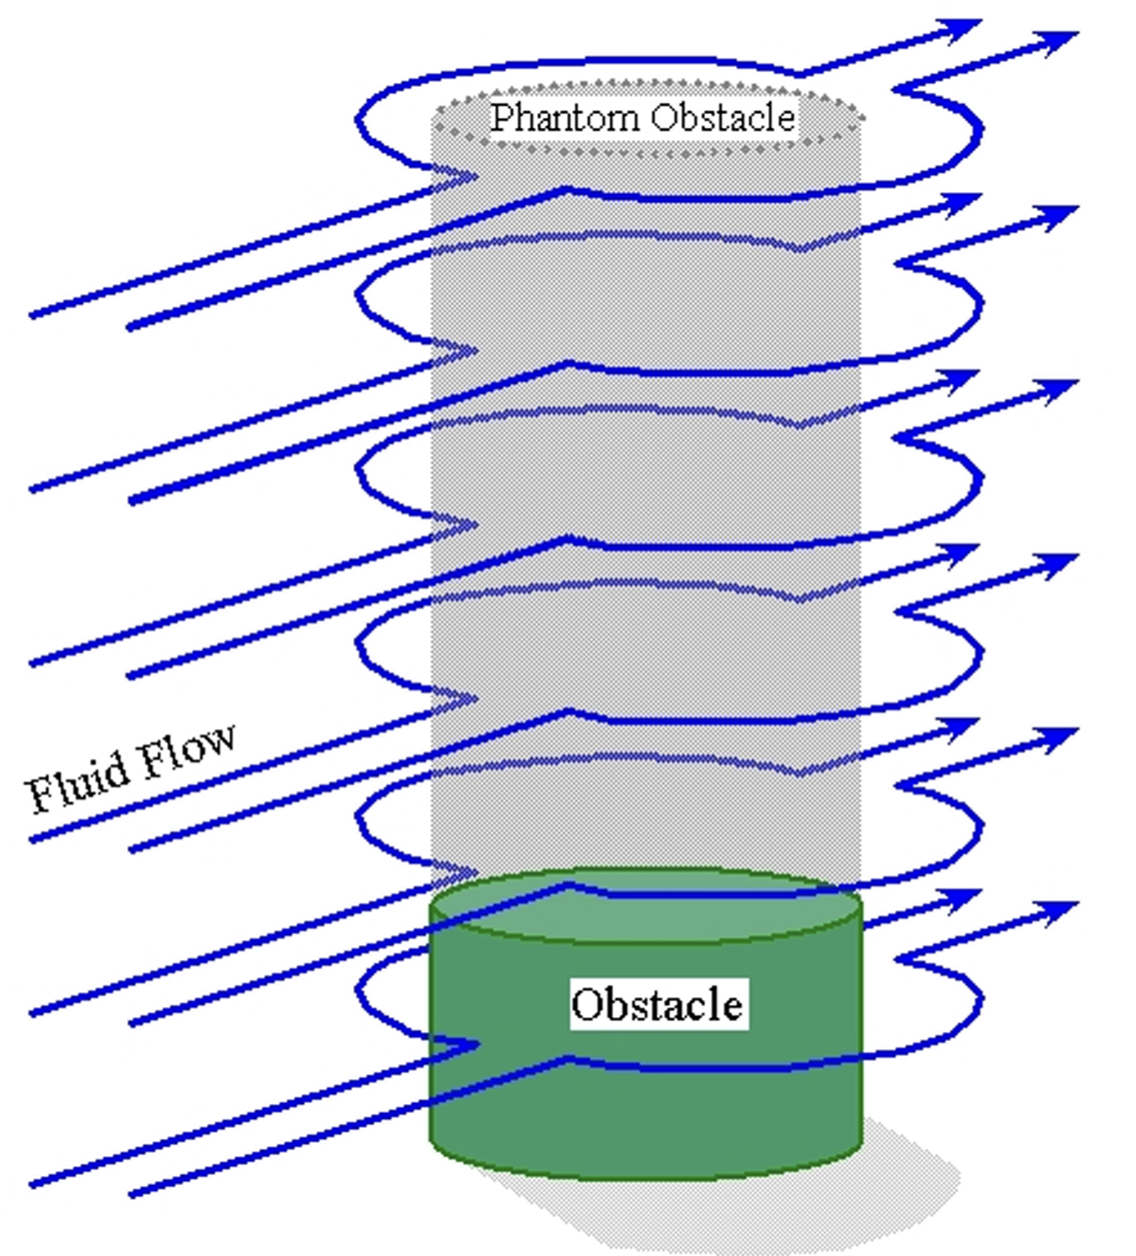
\includegraphics[width=0.5\textwidth,height=\textheight]{figures/TaylorProudmanColumn.png}

}

\caption{\label{fig-taylorproudman}Taylor-Proudman column}

\end{figure}

If rotating fluid moves around an obstacle near the ground, the fluid
must also move around an `imaginary' obstacle higher up in the fluid.
This is depicted in @fig--taylorproudman and can be observed in rotating
tank experiments such as
\href{https://www.youtube.com/watch?v=18HwEHyks9M}{this video}.

\end{tcolorbox}

\hypertarget{sec-thermalwind}{%
\subsection{Thermal wind balance}\label{sec-thermalwind}}

By combining geostrophic and hydrostatic approximations, we arrive at
another important balance in geophysical fluid dynamics, so called
\textbf{thermal wind balance}. To see the balance we simply
differentiate the horizontal geostrophic balance equations
(\ref{eq-horizgeobal}) by \(z\): \[
f\frac{\partial v}{\partial z} = \frac{1}{\bar\rho}\frac{\partial^2 p}{\partial z \partial x}, \quad\quad f\frac{\partial u}{\partial z} = -\frac{1}{\bar\rho}\frac{\partial^2 p}{\partial z \partial y},
\] and combine these with hydrostatic balance from the hydrostatic
Boussinesq equations (\ref{eq-rthydroapprox_hydrobal}) to give
\begin{equation}\protect\hypertarget{eq-thermalwindbalance1}{}{ f\frac{\partial v}{\partial z} = \frac{\partial b}{\partial x} }\label{eq-thermalwindbalance1}\end{equation}
\begin{equation}\protect\hypertarget{eq-thermalwindbalance2}{}{ f\frac{\partial u}{\partial z} = -\frac{\partial b}{\partial y}. }\label{eq-thermalwindbalance2}\end{equation}
These equations represent thermal wind balance and the vertical
derivative of the geostrophic velocity (wind) is known as the thermal
wind. If the buoyancy is constant (e.g., if the density is constant)
then there is no shearing of the geostrophic wind and equations
(\ref{eq-thermalwindbalance1}) - (\ref{eq-thermalwindbalance2}) reduce
to the Taylor-Proudman constraint.

\hypertarget{sec-Geostrophic}{%
\chapter{Geostrophic theory}\label{sec-Geostrophic}}

\hypertarget{overview-2}{%
\section{Overview}\label{overview-2}}

Geophysical fluid dynamics embodies an incredibly wide range of spatial
scales -- from planetary scales of tens of thousand kilometers to
millimeters where the effect of viscosity is felt or clouds and
micro-organisms form. Such a wide spectrum adds to the complexity and
the degrees of freedom in this system and makes the understanding of the
dynamics very challenging. One of our primary tools in geophysical fluid
dynamics is to narrow down our attention to a smaller span of scales,
and then use relevant scaling to reduce the dynamics to something
simpler that is easier to understand or solve. More specifically, if we
consider the scale of thousand kilometers in the atmosphere (or hundreds
of kilometers in the ocean), scaling arguments lead to
\textbf{geostrophic theory}, which is one of the most celebrated results
of geophysical fluid dynamics. The scales of thousand kilometers in the
atmosphere (which are given a special name of \textbf{synoptic scales}
are the range of scales that characterise our daily weather. Hence,
geostrophic theory has been the cornerstone of weather forecast for many
decades. To investigate this theory, we start by introducing the
appropriate scaling for different variables and then use asymptotic
expansion to simplify the dynamics.

\hypertarget{scaling-the-equations-and-rossby-number}{%
\section{Scaling the equations and Rossby
number}\label{scaling-the-equations-and-rossby-number}}

The goal of scaling is to understand the relative importance of
different phenomena that influence the fluids motion. In geophysical
fluids, we have seen that stratification and rotation play crucial roles
in the dynamics. The characteristic length scale that marks the relative
importance of these two phenomena is the \emph{deformation radius} (also
known as Rossby radius of deformation) defined as
\begin{equation}\protect\hypertarget{eq-def_radius}{}{
    \Ld = \frac{N \mathcal{H}}{f_0},
}\label{eq-def_radius}\end{equation} where \(\mathcal{H}\) is the
vertical scale (\(f\) and \(N\) are Coriolis and Brunt--Väisälä
frequencies introduced in previous chapters). Recall that
stratification/buoyancy primarily acts in the vertical, whereas the
leading order Coriolis force \(f \eb_z \times \vb\) acts in the
horizontal. Hence, \(\Ld\) characterises the horizontal scale at which
rotational effects become as important as buoyancy effects. In the
atmosphere, the ratio \(N/f\) is typically of order 100, so for a
vertical scale associated with the height of the tropopause (first layer
of the atmosphere where the weather dynamics take place), \(\Ld = 1000\)
km. In synoptic or weather scales, we consider horizontal scales that
close \(\Ld\) or slightly larger. The deformation radius of the ocean is
an order of magnitude smaller than that of the atmosphere because
\(N/f\) is much smaller in the ocean. Hence, the order of hundred
kilometer in the ocean is dynamically equivalent to thousand kilometer
in the atmosphere.

We scale the flow variables with the following characteristic values \[
   (x,y) = {\mathcal{L}}{({x^*},{y^*})}, \quad z = {\mathcal{H}}{\zh} , \quad t = {\mathcal{T}}{\tha} , \quad  (u,v) =  {\mathcal{U}}{(\nd{u},\nd{v})}, \quad w = {\mathcal{W}}{\wh},,
\] \begin{equation}\protect\hypertarget{eq-scaling}{}{
p = {\mathcal{P}}{\ph} , \quad b = {\mathcal{B}}{\bh} , \quad \fb = {f_0}{\nd{\boldsymbol{f}}} , 
}\label{eq-scaling}\end{equation} where \(\nd{()}\) are dimensionless.
We also use \(\gradH = 1/ \mathcal{L} \ \nd{\nabla}_H\), consistent with
the scale of \(x\) and \(y\). We then non-dimensionalise the
(hydrostatic) Boussinesq equations
\begin{equation}\protect\hypertarget{eq-nd_BousmomH}{}{
\frac{1}{f_0 \mathcal{T}} \frac{\partial\vh}{\partial \tha} + \frac{\mathcal{U}}{f_0 \mathcal{L}} \ (\vh \cdot \gradHh ) \vh + \frac{\mathcal{W}}{f_0 \mathcal{H}} \wh \frac{\partial \vh }{\partial \zh} + \fh \times \vh = - \frac{\mathcal{P}}{\bar\rho f_0 \mathcal{L}\ \mathcal{U} } \ \gradHh \ph,}\label{eq-nd_BousmomH}\end{equation}
\begin{equation}\protect\hypertarget{eq-nd_BousmomV}{}{ \frac{\bar\rho \mathcal{B} \mathcal{H}}{\mathcal{P}} \ \bh = \frac{\partial \ph }{\partial \zh} ,}\label{eq-nd_BousmomV}\end{equation}
\begin{equation}\protect\hypertarget{eq-nd_Bousdiv}{}{ \gradHh \cdot\vh + \frac{\mathcal{W} \mathcal{L}}{\mathcal{U} \mathcal{H}}  \frac{\partial \wh}{\partial \zh} =0, }\label{eq-nd_Bousdiv}\end{equation}
\begin{equation}\protect\hypertarget{eq-nd_Bousbuoy}{}{\frac{1}{f_0 \mathcal{T}} \frac{\partial \bh}{\partial \tha} + \frac{\mathcal{U}}{f_0 \mathcal{L}} \ (\vh\cdot\gradHh ) \bh + \frac{\mathcal{W}}{f_0 \mathcal{H}} \wh \frac{\partial \bh}{\partial \zh} + \frac{N^2 \mathcal{W}}{\mathcal{B}} \wh =0.}\label{eq-nd_Bousbuoy}\end{equation}

\begin{tcolorbox}[enhanced jigsaw, toprule=.15mm, left=2mm, opacityback=0, breakable, arc=.35mm, colback=white, rightrule=.15mm, bottomrule=.15mm, colframe=quarto-callout-note-color-frame, leftrule=.75mm]
\begin{minipage}[t]{5.5mm}
\textcolor{quarto-callout-note-color}{\faInfo}
\end{minipage}%
\begin{minipage}[t]{\textwidth - 5.5mm}

We could have started from non-hydrotatic Boussinesq equations as well
and by a scaling argument shows that the vertical momentum equation at
the leading order is hydrostatic.

\end{minipage}%
\end{tcolorbox}

In Equations (\ref{eq-nd_BousmomH}) - (\ref{eq-nd_Bousbuoy}) one of the
most important dimensionless parameters in geophysical fluid dynamics
has surface \begin{equation}\protect\hypertarget{eq-def_Ro}{}{
     \Ro = \frac{\mathcal{U}}{f_0 \mathcal{L}},
}\label{eq-def_Ro}\end{equation} which shows the ratio of inertial force
to Coriolis force and is called \textbf{Rossby number}. If the Coriolis
force is strong, we expect \(\Ro\) to be small. Using the definition
Rossby number (\ref{eq-def_Ro}), we rewrite (\ref{eq-nd_BousmomH}) -
(\ref{eq-nd_Bousbuoy}) as
\begin{equation}\protect\hypertarget{eq-nd_BousmomH2}{}{ \frac{1}{f_0 \mathcal{T}} \frac{\partial\vh}{\partial \tha} + \Ro \ (\vh \cdot \gradHh ) \vh + \Ro \frac{\mathcal{W} \mathcal{L}}{\mathcal{U} \mathcal{H}} \wh \frac{\partial \vh }{\partial \zh} + \fh \times \vh = - \frac{\mathcal{P}}{\bar\rho f_0 \mathcal{L}\ \mathcal{U} } \ \gradHh \ph, }\label{eq-nd_BousmomH2}\end{equation}
\begin{equation}\protect\hypertarget{eq-nd_BousmomV2}{}{ \frac{\bar\rho \mathcal{B} \mathcal{H}}{\mathcal{P}} \ \bh = \frac{\partial \ph }{\partial \zh} , }\label{eq-nd_BousmomV2}\end{equation}
\begin{equation}\protect\hypertarget{eq-nd_Bousdiv2}{}{ \gradHh \cdot\vh + \frac{\mathcal{W} \mathcal{L}}{\mathcal{U} \mathcal{H}}  \frac{\partial \wh}{\partial \zh} =0,}\label{eq-nd_Bousdiv2}\end{equation}
\begin{equation}\protect\hypertarget{eq-nd_Bousbuoy2}{}{ \frac{1}{f_0 \mathcal{T}} \frac{\partial \bh}{\partial \tha} +\Ro \ (\vh\cdot\gradHh ) \bh + \Ro \frac{\mathcal{W} \mathcal{L}}{\mathcal{U} \mathcal{H}} \wh \frac{\partial \bh}{\partial \zh} + \frac{N^2 \mathcal{W}}{\mathcal{B}} \wh =0. }\label{eq-nd_Bousbuoy2}\end{equation}

In the rest of this chapter we assume \(N\) to be constant. However, the
geostrophic theory can be easily generalised to a variable \(N\).

\begin{tcolorbox}[enhanced jigsaw, toprule=.15mm, left=2mm, opacityback=0, breakable, arc=.35mm, colback=white, rightrule=.15mm, bottomrule=.15mm, colframe=quarto-callout-note-color-frame, leftrule=.75mm]
\begin{minipage}[t]{5.5mm}
\textcolor{quarto-callout-note-color}{\faInfo}
\end{minipage}%
\begin{minipage}[t]{\textwidth - 5.5mm}

\(Ro\) is named after after the Swedish-American meteorologist
Carl-Gustav Arvid Rossby, who first explain who first explained the
large-scale motions of the atmosphere using fluid mechanics.

\end{minipage}%
\end{tcolorbox}

\hypertarget{leading-order-geostrophic-balance}{%
\section{Leading order: geostrophic
balance}\label{leading-order-geostrophic-balance}}

Our goal in this section is to use the relevant scaling to the weather
scale to simplify the Bousinesq equation. To that end, we consider the
following assumptions

\begin{enumerate}
\def\labelenumi{\arabic{enumi}.}
\tightlist
\item
  The Rossby number is small and we denote it by \(\Ro =\epsilon\) to
  emphasise this fact. This means the Coriolis effect is strong. The
  average wind speed in the atmosphere is about \(8 m/s\), the Coriolis
  parameter at mid-latitudes (about \(35^{\circ}\)) is
  \(0.8 \times 10^{-4}\) and as mentioned earlier we are considering the
  weather (synoptic) scales of \(\mathcal{L} = 1000 km\). With these
  values we get \(\Ro \approx 0.1\), which is indeed a small parameter.
  A similar calculation for the ocean scales of 100 km leads to even
  smaller Rossby numbers.
\item
  The horizontal scale of motion is not significantly larger than the
  deformation radius (Equation~\ref{eq-def_radius}). More specifically,
  \[\frac{\Ld}{\mathcal{L}} = O(1) \] This is a direct translation of
  considering the synoptic scales (thousands of kilometers) in the
  atmosphere or the mesoscales (hundreds of kilometers) in the ocean.
\item
  The time scale is \(\mathcal{T}=\mathcal{L}/\mathcal{U}\). This time
  scale sometimes is referred to as \emph{eddy turnover} time, because
  if we consider an eddy or vortex with the velocity \(\mathcal{U}\) and
  diameter \(\mathcal{L}\), it will roughly take
  \(\mathcal{L}/\mathcal{U}\) time to make a full turn. This time scale
  is also known as \emph{inertial} or \emph{advective} time scale,
  because it will make the inertial or advection term
  \(\vb \cdot \grad \vb\) the same order of magnitude as the time
  derivative. This assumption leads to \(1/(\mathcal{T}f_0)=\Ro\) in
  (\ref{eq-nd_BousmomH2}) - (\ref{eq-nd_Bousbuoy2}) .
\item
  To keep \(\partial w / \partial z\) in the continuity equation
  Equation~\ref{eq-nd_Bousdiv2}, we assume the vertical velocity scales
  as \(\mathcal{W} = \mathcal{U} \mathcal{H} / \mathcal{L}\). This is
  simply keeping the problem in more general form by allowing
  \(\partial w / \partial z\) to exist at the leading order rather than
  imposing an extra assumption. In other words, such scaling allows
  \(\mathcal{W} < \mathcal{U} \mathcal{H} / \mathcal{L}\) as the terms
  \(\partial w / \partial z\) and \(w \partial / \partial z\) may
  naturally become small or zero in the solution (our scaling does not
  prevent).
\item
  The beta effect is an order (\(\epsilon\)) smaller than the \(f_0\).
  More precisely,
  \[ \fh = \left( \frac{f_0 + \beta \nd{y} \mathcal{L}}{f_0} \right) \eb_z =  \left( 1 + \frac{\beta \mathcal{L}}{f_0} \nd{y} \right) \eb_z =  \left( \nd{f}_0 + \epsilon \ \nd{\beta} \nd{y} \right) \eb_z
  \] where \(\nd{\beta}\) is \(O(1)\) due to the assumption made and
  \(\nd{f}_0 = f_0/f_0 = 1\). Note that we still keep \(\nd{f}_0\) in
  the equations (despite being simply 1) so the leading term of the
  Coriolis force will stand out in the non-dimensionalised equations.
  Likewise, we keep \(\fh_0 = \nd{f}_0 \eb_z\) instead of the unit
  vector \(\eb_z\).
\end{enumerate}

Using the assumption 3, 4 and 5, we rewrite (\ref{eq-nd_BousmomH2}) -
(\ref{eq-nd_Bousbuoy2})
\begin{equation}\protect\hypertarget{eq-nd_BousmomH3}{}{ \epsilon \left(  \frac{\partial\vh}{\partial \tha} + (\vh \cdot \gradHh ) \vh + \wh \frac{\partial \vh }{\partial \zh} \right) +  (\nd{f}_0 + \epsilon \nd{\beta} \nd{y})  \eb_z \times \vh = - \frac{\mathcal{P}}{\bar\rho f_0 \mathcal{L}\ \mathcal{U} } \ \gradHh \ph, }\label{eq-nd_BousmomH3}\end{equation}
\begin{equation}\protect\hypertarget{eq-nd_BousmomV3}{}{ \frac{\bar\rho \mathcal{B} \mathcal{H}}{\mathcal{P}} \ \bh = \frac{\partial \ph }{\partial \zh}, }\label{eq-nd_BousmomV3}\end{equation}
\begin{equation}\protect\hypertarget{eq-nd_Bousdiv3}{}{ \gradHh \cdot\vh + \frac{\partial \wh}{\partial \zh} =0, }\label{eq-nd_Bousdiv3}\end{equation}
\begin{equation}\protect\hypertarget{eq-nd_Bousbuoy3}{}{ \epsilon \left(\frac{\partial \bh}{\partial \tha} +(\vh\cdot\gradHh ) \bh + \wh \frac{\partial \bh}{\partial \zh}  \right) + \frac{N^2 \mathcal{W}}{\mathcal{B}}\wh =0. }\label{eq-nd_Bousbuoy3}\end{equation}

If we consider the limit of small \(\epsilon\) (following assumption 1),
in the horizontal momentum Equation~\ref{eq-nd_BousmomH3} the Coriolis
force will be larger than all other terms in the LHS. We know the
Coriolis force is not small at the weather scale as the horizontal wind
\(\vb\) is not negligible. Hence, the pressure gradient in the RHS has
to be the same order as Coriolis force to balance it out. This require
the following scaling for pressure \[
    \mathcal{P} \sim \bar\rho f_0 \mathcal{L}\ \mathcal{U}
\] Following this scaling, we can move to the vertical momentum
Equation~\ref{eq-nd_BousmomV3} and infer the approperiate scaling for
buoyancy \[
    \mathcal{B} \sim \frac{f_0 \mathcal{L}\ \mathcal{U}}{\mathcal{H}}
\] After replacing for \(\mathcal{B}\) and \(\mathcal{P}\) all the
pieces of scaling puzzle are complete and we have a set of equations for
which we know the relative importance of all terms
\textbackslash begin\{align\}
\begin{equation}\protect\hypertarget{eq-nd_BousmomH4}{}{ \epsilon \left(  \frac{\partial\vh}{\partial \tha} + (\vh \cdot \gradHh ) \vh + \wh \frac{\partial \vh }{\partial \zh} \right) +  \fh_0 \times \vh + \epsilon \nd{\beta} \nd{y} \eb_z \times \vh = - \gradHh \ph, }\label{eq-nd_BousmomH4}\end{equation}
\begin{equation}\protect\hypertarget{eq-nd_BousmomV4}{}{ \bh = \frac{\partial \ph }{\partial \zh}, }\label{eq-nd_BousmomV4}\end{equation}
\begin{equation}\protect\hypertarget{eq-nd_Bousdiv4}{}{ \gradHh \cdot\vh + \frac{\partial \wh}{\partial \zh} =0, }\label{eq-nd_Bousdiv4}\end{equation}
\begin{equation}\protect\hypertarget{eq-nd_Bousbuoy4}{}{ \epsilon \left(\frac{\partial \bh}{\partial \tha} +(\vh\cdot\gradHh ) \bh + \wh \frac{\partial \bh}{\partial \zh}  \right) + \left( \frac{\Ld}{\mathcal{L}} \right)^2 \wh =0. }\label{eq-nd_Bousbuoy4}\end{equation}
where we have used the definition of deformation radius.

In the next step, we start with the classical asymptotic approach to
reduce the above equations to a simpler set. We expand all variables in
terms of \(\epsilon\) \[
    \vh = \vh_0 + \epsilon \vh_1 + \dots, \quad \wh = \wh_0 + \epsilon \wh_1 + \dots, \quad
    \ph = \ph_0 + \epsilon \ph_1 + \dots, \quad \bh = \bh_0 + \epsilon \bh_1 + \dots  
\] Upon substitution in Equation~\ref{eq-nd_BousmomH4} and keeping the
leading order terms (the smallest power of \(\epsilon\)), we find
\begin{equation}\protect\hypertarget{eq-geobalance}{}{  \fh_0 \times \vh_0 = - \gradH \ph_0, }\label{eq-geobalance}\end{equation}

This is the infamous \textbf{geostrophic balance}, which is the building
block of modern weather forecast. It expresses that the Coriolis forces
is balancing the pressure gradient. If we take the divergence of both
sides in Equation~\ref{eq-geobalance}, we find
\begin{equation}\protect\hypertarget{eq-divfree_geo}{}{  \gradHh \cdot\vh_0 = 0, }\label{eq-divfree_geo}\end{equation}
which tells us that the horizontal velocity is divergence-free at the
leading order. As a result, we can define the streamfunction below
\begin{equation}\protect\hypertarget{eq-streamfunction_geo}{}{ \nd{u}_0 = - \frac{\partial \psih}{\partial \nd{y}}, \quad \nd{v}_0 = \frac{\partial \psih}{\partial \nd{x}}. }\label{eq-streamfunction_geo}\end{equation}
This looks similar to the definition of streamfunction for 2D
incompressible flow. However, unlike 2D flow, \(\psih\), \(\nd{u}_0\)
and \(\nd{v}_0\) can depend on \(z\). Considering
Equation~\ref{eq-geobalance}, we can set \[
    \nd{\psi} = \ph_0/f_0,
\] which automatically satisfies Equation~\ref{eq-streamfunction_geo}.
At leading order, Equation~\ref{eq-nd_Bousdiv4} becomes
\begin{equation}\protect\hypertarget{eq-hydstat_balance}{}{   \bh_0 = \frac{\partial \ph_0}{\partial z} }\label{eq-hydstat_balance}\end{equation}
This is simply the \textbf{hydrostatic balance}. Consider the
conservation of mass at leading order \[
    \gradHh \cdot\vh_0 + \frac{\partial \wh_0}{\partial \zh} = 0.
\] We have already established that \(\gradHh \cdot\vh_0 = 0\) in
Equation~\ref{eq-divfree_geo}. Hence,
\begin{equation}\protect\hypertarget{eq-dw0dz_geo}{}{ \frac{\partial \wh_0}{\partial \zh} = 0, }\label{eq-dw0dz_geo}\end{equation}
implying that if \(\wh_0\) is zero somewhere (like at the boundary) then
it is zero everywhere.

Considering the assumption 2, the buoyancy
Equation~\ref{eq-nd_Bousbuoy4} at leading order is
\begin{equation}\protect\hypertarget{eq-w0_geo}{}{ \left( \frac{\Ld}{\mathcal{L}} \right)^2 \wh_0 = 0, }\label{eq-w0_geo}\end{equation}
showing that the leading order the vertical velocity is zero.

\begin{tcolorbox}[enhanced jigsaw, toprule=.15mm, left=2mm, opacityback=0, breakable, arc=.35mm, colback=white, rightrule=.15mm, bottomrule=.15mm, colframe=quarto-callout-note-color-frame, leftrule=.75mm]
\begin{minipage}[t]{5.5mm}
\textcolor{quarto-callout-note-color}{\faInfo}
\end{minipage}%
\begin{minipage}[t]{\textwidth - 5.5mm}

Note that Equation~\ref{eq-w0_geo} is in a sense stronger than
Equation~\ref{eq-dw0dz_geo}, but it requires
\({\Ld}/\mathcal{L} = O(1)\). For \(\mathcal{L}>{\Ld}\), all the leading
order results hold (geostrophic and hydrostatic balance), except
Equation~\ref{eq-w0_geo}. This range scale correspond to planetary
scales.

\end{minipage}%
\end{tcolorbox}

As discussed earlier in Section~\ref{sec-thermalwind}, we can also
combined hydrostatic and geostrophic balance by taking the
\(z\)-derivative of Equation~\ref{eq-geobalance} and substitute for
pressure terms from Equation~\ref{eq-hydstat_balance}
\begin{equation}\protect\hypertarget{eq-thermalwind_balance}{}{  \fh_0 \times \frac{\partial \vh_0}{\partial \nd{z}} = - \gradH \bh_0 }\label{eq-thermalwind_balance}\end{equation}
which is the \emph{thermal wind balance} that holds at leading order.

We take a short break here from asymptotics and look at the implications
and applications of geostrophic balance before proceeding to the next
order.

\hypertarget{geostrophic-balance-and-weather-forecast}{%
\subsection{Geostrophic Balance and weather
forecast}\label{geostrophic-balance-and-weather-forecast}}

Equation~\ref{eq-geobalance} is one of the most important equations in
the large scale atmospheric physics and weather forecast. For example by
knowing the pressure distribution, we can find the geostrophic velocity
using this equation. \(- \gradH p_0\) in meteorology is known as
\emph{pressure gradient force} (PGF), the direction of which is from
high to low pressure. This can be slightly confusing as the pressure
gradient itself \(\gradH p_0\) is in the opposite direction to PGF, but
consider the force that fluid parcel feels is from high to low pressure.
Knowing PGF and using cross product rule in
Equation~\ref{eq-geobalance}, we find that if \(\fb\) points upward (or
out of the horizontal plane), when we face the direction of PGF, the
geostrophic velocity should be to our right. This is the case in the
Northern hemisphere where \(\fb\) points upward. The situation is
reversed in the Southern hemisphere as \(\fb\) points downward. For
instance, if the PGF is pointing northward in the Southern hemisphere,
the geostrophic wind blows toward the west. Following this argument, we
also find that the geostrophic velocity is aligned with
constant-pressure contours known as \emph{isobar}. As illustrated in the
example offigure Figure~\ref{fig-weathermap}, using the direction of PGF
we can find the direction of geostrophic velocity on weather maps
(pressure contours)

\begin{figure}

{\centering 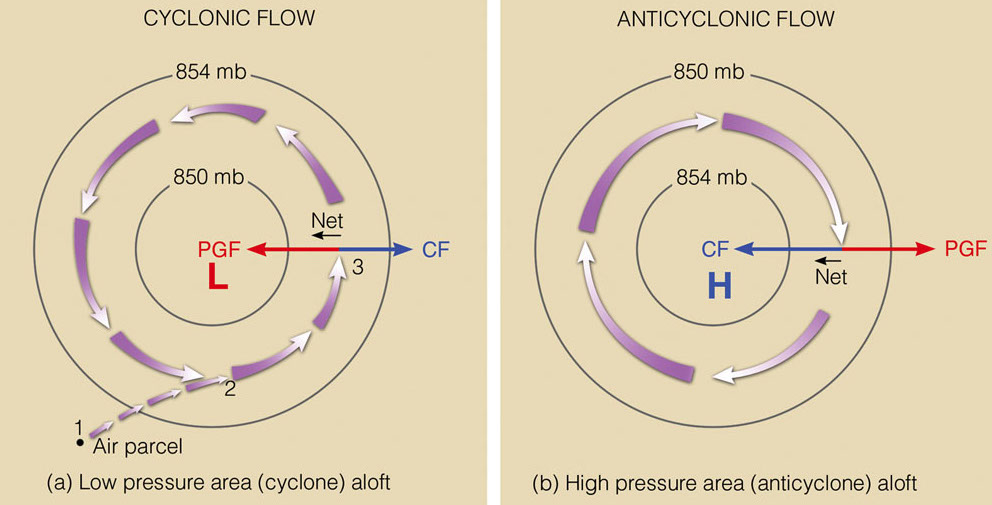
\includegraphics[width=0.85\textwidth,height=\textheight]{figures/cyc_anticyc_schem.jpeg}

}

\caption{\label{fig-cycanticyc_schem}The direction of motion caused by
geostrophic wind in cyclone (left) and anticyclone (right) in the
Northern hemisphere.}

\end{figure}

\begin{figure}

\begin{minipage}[t]{0.50\linewidth}

{\centering 

\raisebox{-\height}{

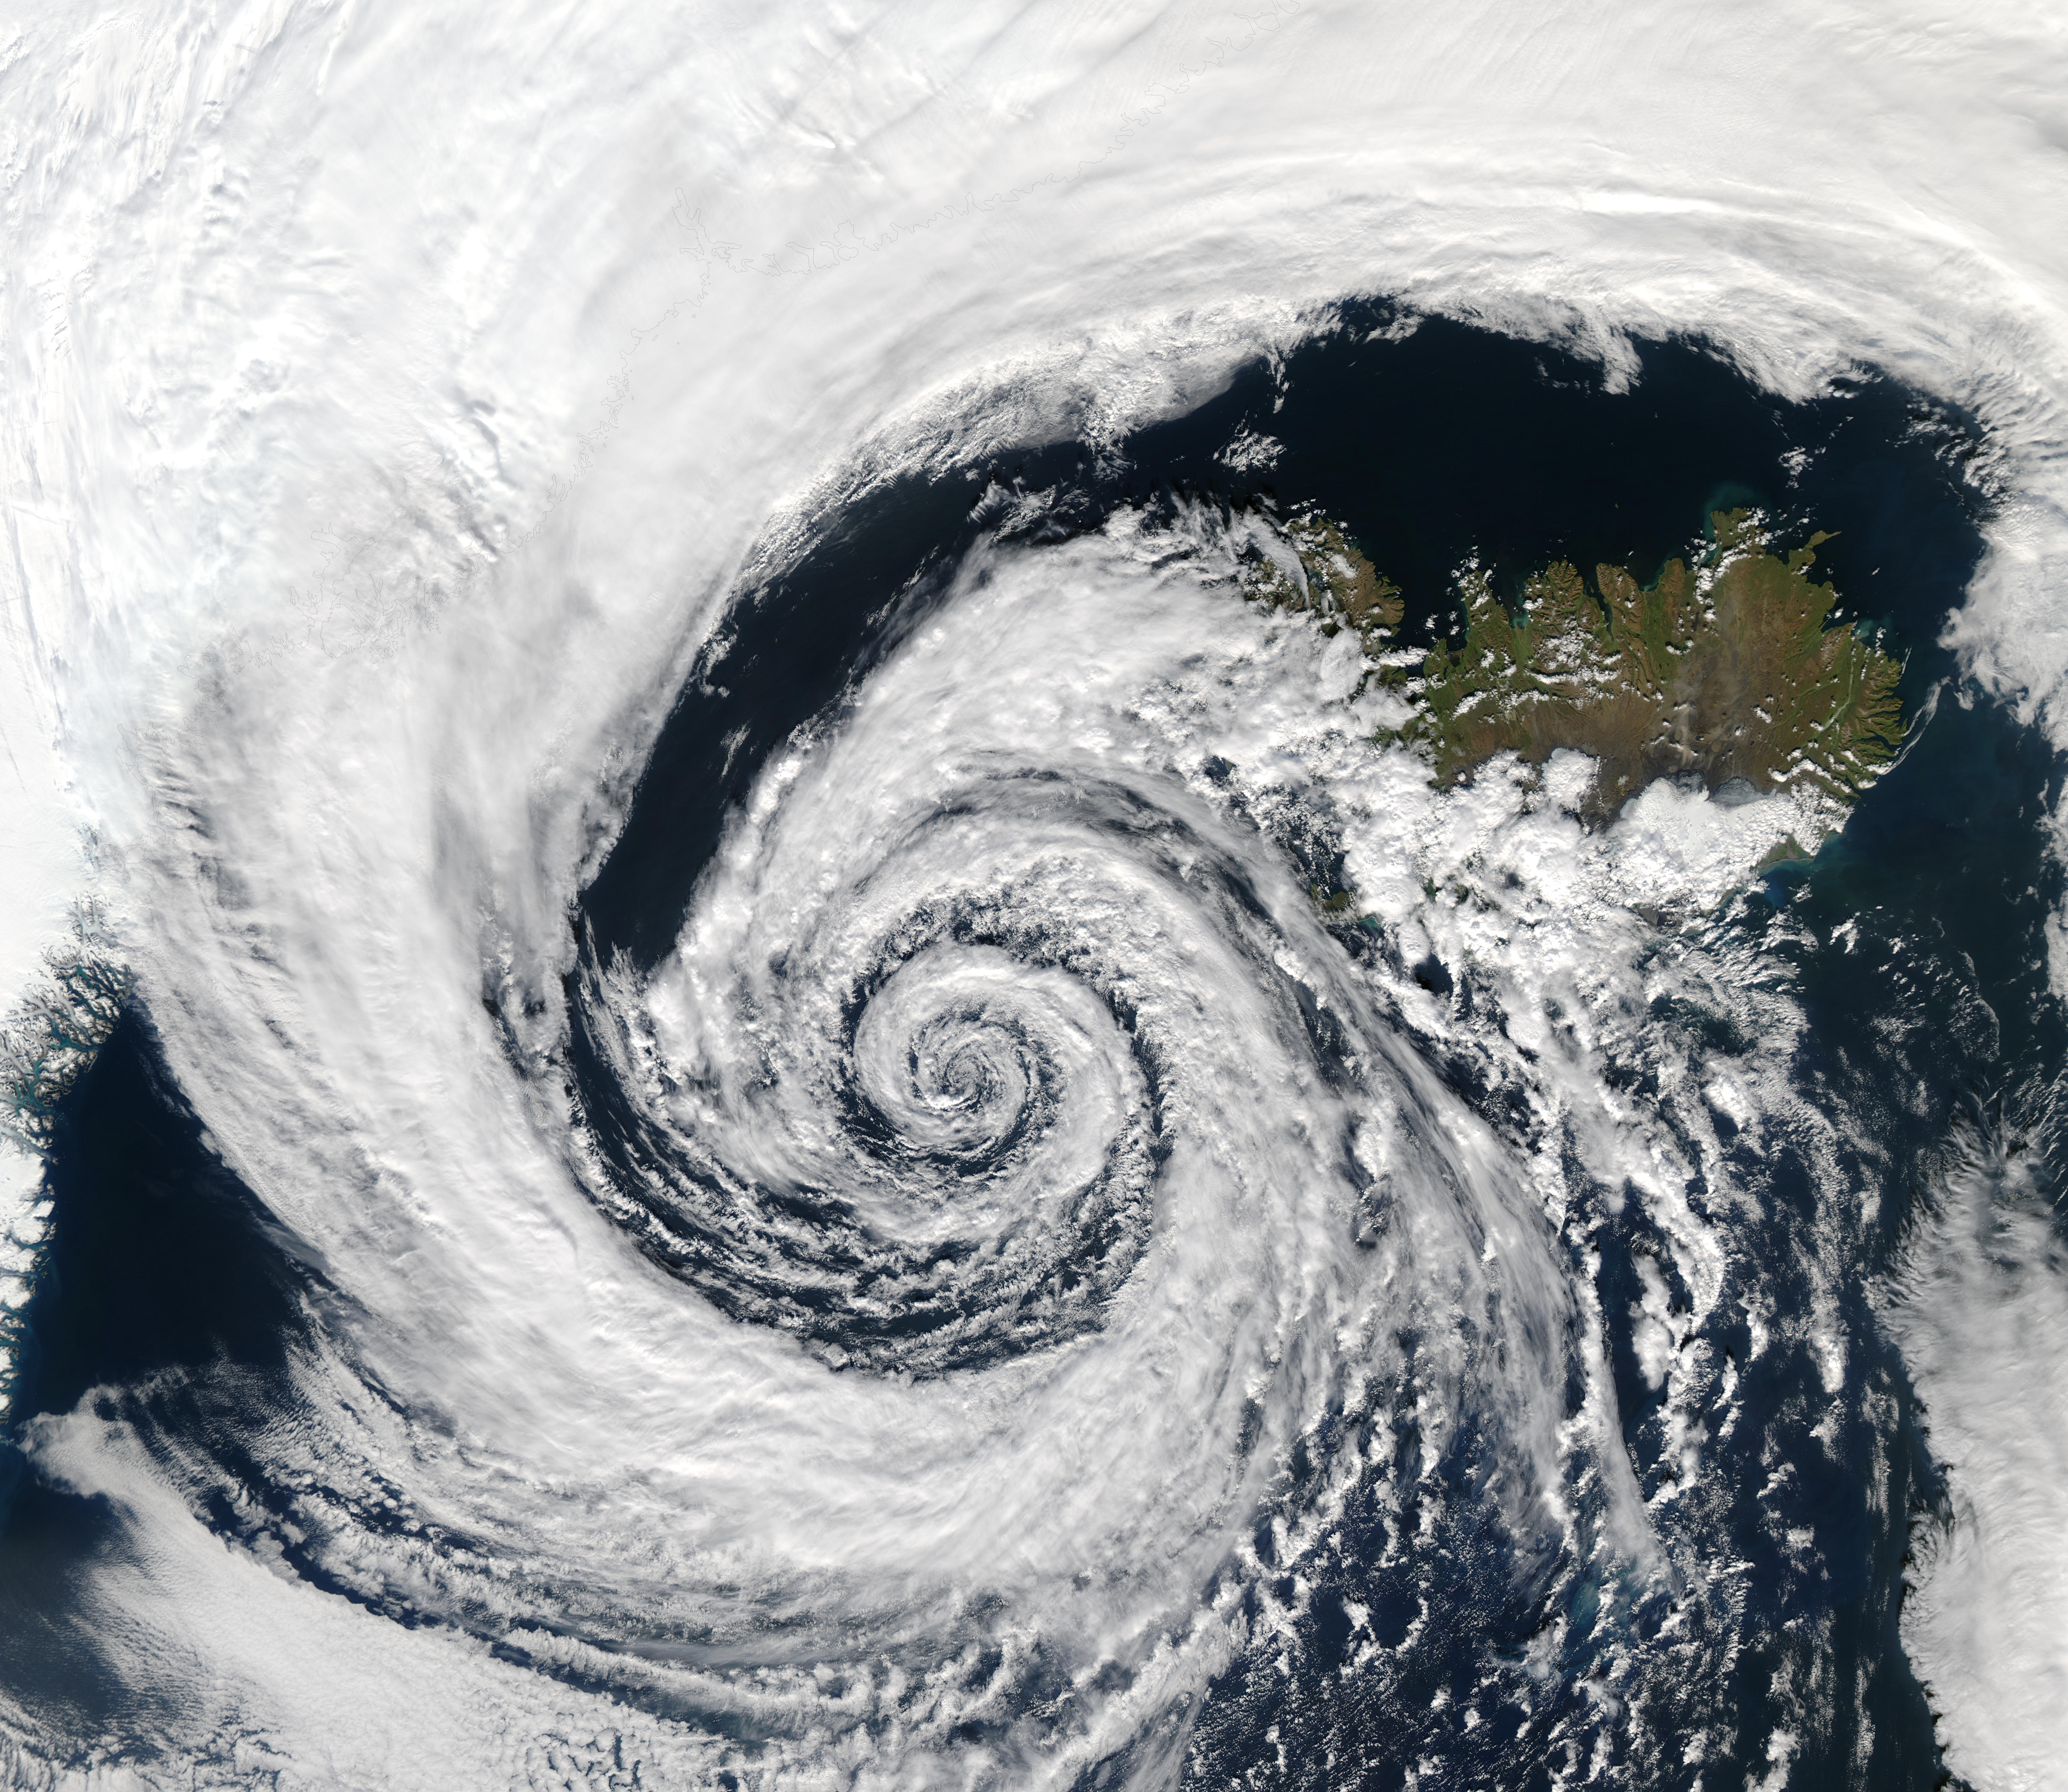
\includegraphics{figures/Low_Pressure.jpg}

}

}

\end{minipage}%
%
\begin{minipage}[t]{0.50\linewidth}

{\centering 

\raisebox{-\height}{

\includegraphics{figures/High_Pressure2.jpg}

}

}

\end{minipage}%

\caption{\label{fig-satellite_image}Satellite images of a cyclone
(low-pressure system) in the left panel and an anticyclone
(high-pressure system) in the right panel.}

\end{figure}

\begin{figure}

{\centering 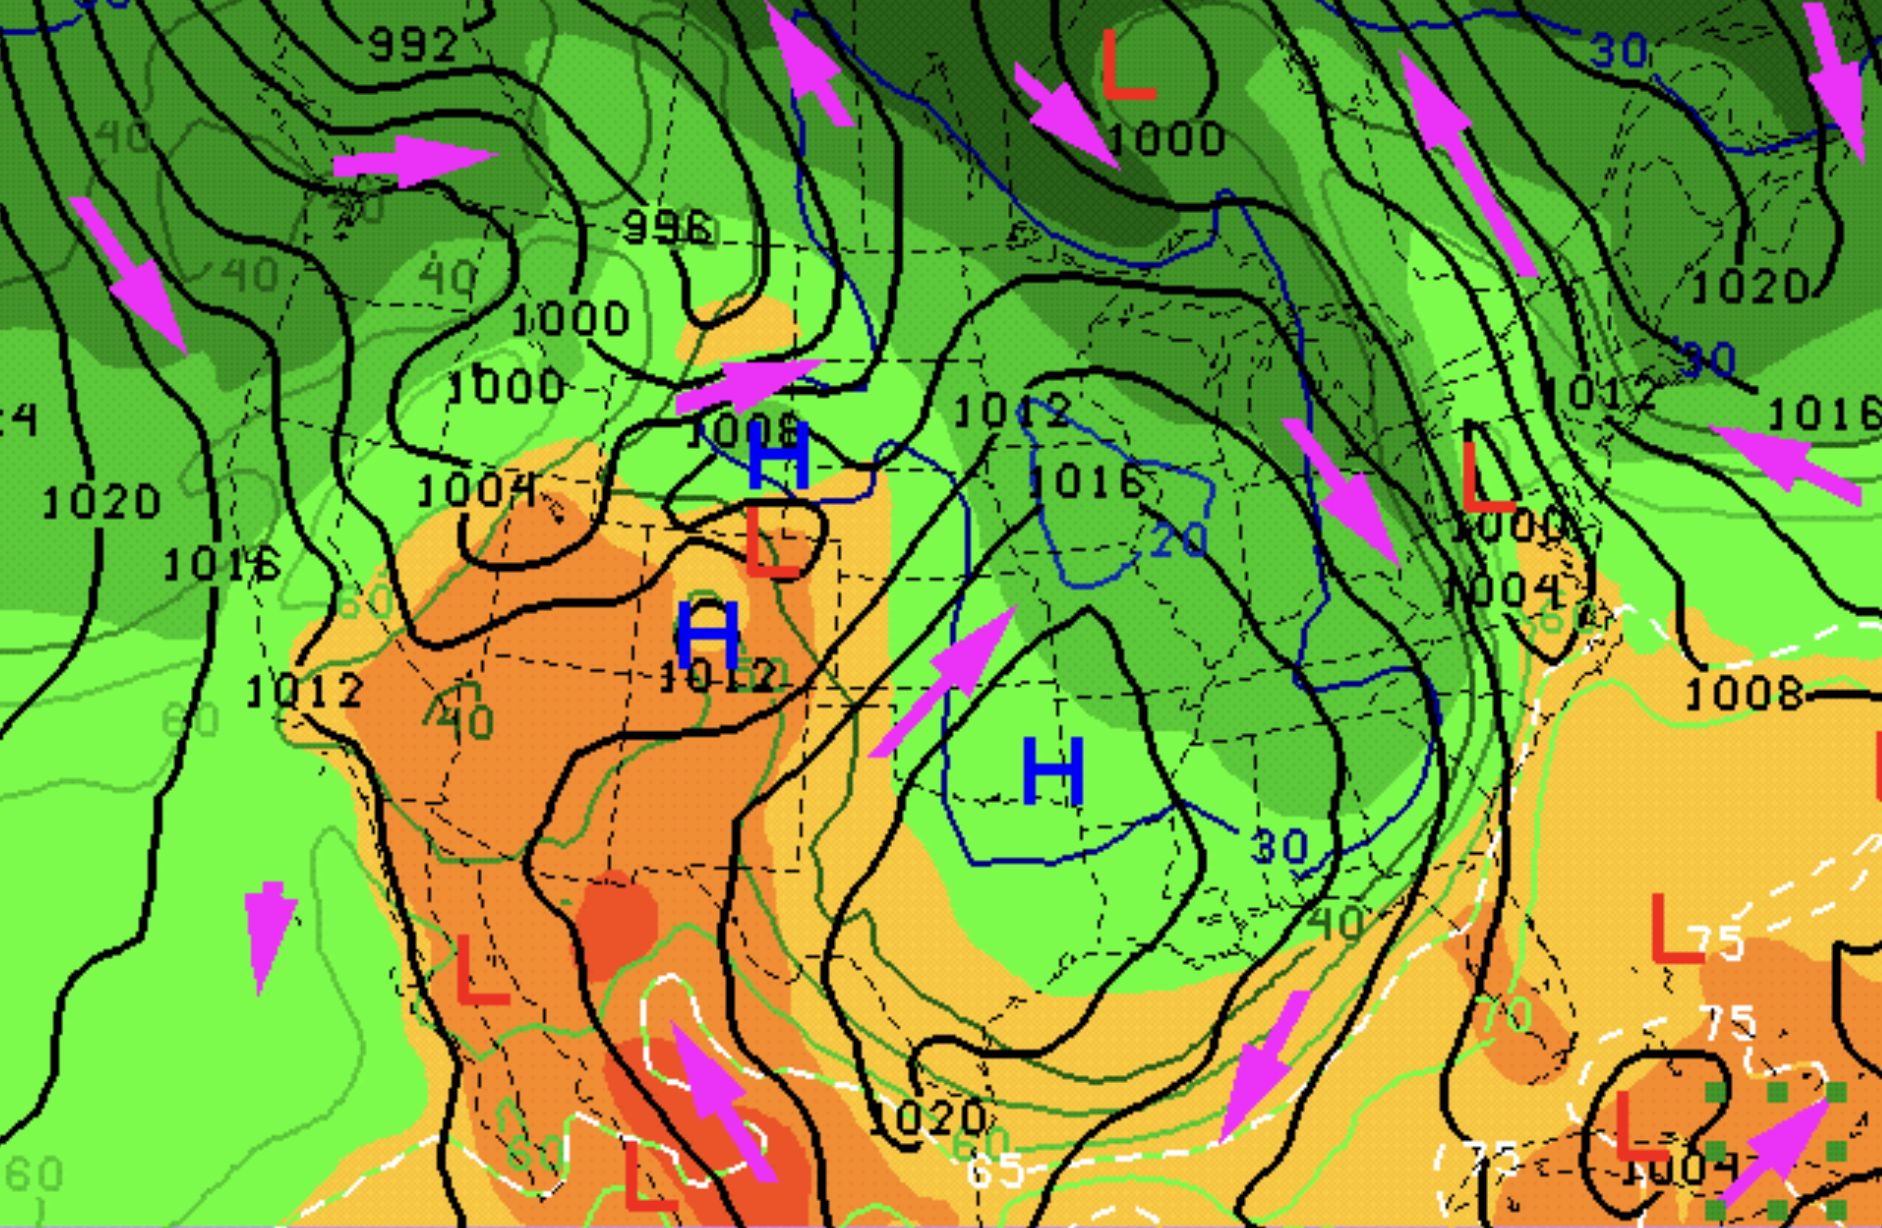
\includegraphics[width=0.65\textwidth,height=\textheight]{figures/weathermap_geowind.png}

}

\caption{\label{fig-weathermap}Pressure contours (isobars) on a weather
map (in Northern hemisphere). The magenta arrows show the direction of
geostrophic velocity.}

\end{figure}

The geostrophic balance is also fundamental in understanding the
pressure systems. These systems are basically giant vorticies that form
our weather. For the moment, let's consider the Northern hemisphere. In
a high pressure system, the pressure increase as we move toward the
centre (see figure). Hence, PGF points outward. As a result, the fluid
parcels should rotate clockwise in this system as shown in
Figure~\ref{fig-cycanticyc_schem} (following our argument in the
preceding paragraph). This system is known as \emph{anticyclone}. In
contrast, the direction of motion is anticlockwise in a low-pressure
system (see Figure~\ref{fig-cycanticyc_schem}), which is known as
\emph{cyclone}. With a similar reasoning we find out that cyclones
(low-pressure systems) move anticlockwise and anticyclones
(high-pressure systems) move clockwise in the Southern hemisphere. When
a cyclone moves over sea, it absorbs moisture into its core as it has
low pressure compared to its surrounding. This moisture turns into cloud
and is carried in-land and create rainy weather. Hence, low-pressure
systems (cyclones) are associated with rain and clouds and high-pressure
systems with sunny weather. Such characteristics of these systems are
beautifully capture in satellite images such as those shown in
Figure~\ref{fig-satellite_image}. The clouds are attracted toward the
centre of cyclone, whereas they are repelled from the centre of
anticyclone.

\begin{tcolorbox}[enhanced jigsaw, toprule=.15mm, left=2mm, opacityback=0, breakable, arc=.35mm, colback=white, rightrule=.15mm, bottomrule=.15mm, colframe=quarto-callout-note-color-frame, leftrule=.75mm]
\begin{minipage}[t]{5.5mm}
\textcolor{quarto-callout-note-color}{\faInfo}
\end{minipage}%
\begin{minipage}[t]{\textwidth - 5.5mm}

The thermodynamics behind the formation of cyclones/anticyclones is
beyond the scope of this course but is an important area of study in
meteorology. More particularly, development or strengthening of cyclones
in the atmosphere can lead to the formation of hurricanes (this branch
of science is so important that is given a name: \emph{Cyclogenesis}).

\end{minipage}%
\end{tcolorbox}

\hypertarget{sec-QGBouss}{%
\section{Next order: quasigeostrophy}\label{sec-QGBouss}}

The leading order asymptotics revealed very useful information about the
geostrophic balance and vertical velocity. However, these relations are
\emph{diagnostic} and time independent. In other words, they show, for
example, how velocity is related to pressure but they do not show how
velocity or pressure evolve in time. We know that the large scale
atmosphere and ocean are dynamic and change in time. Hence, to find the
time evolution of the flow variables we have to go to the next order
(i.e.~\(O(\epsilon)\)).

Starting with horizontal momentum equation
Equation~\ref{eq-nd_BousmomH4}, we find \[
    \frac{\partial\vh_0}{\partial \tha} + (\vh_0 \cdot \gradHh ) \vh_0 + \nd{\beta} \nd{y} \eb_z \times \vh_0 + \fh_0 \times \vh_1 = - \gradHh \ph_1.
\] We then take the curl of this equation \begin{align*}
        \frac{\partial}{\partial \nd{x}} \left( \frac{\partial \nd{v}_0}{\partial \tha} + \nd{u}_0 \frac{\partial \nd{v}_0}{\partial \nd{x}} + \nd{v}_0 \frac{\partial \nd{v}_0}{\partial \nd{y}} + \nd{\beta} \nd{y} u_0 + \nd{f}_0 u_1  \right) 
        &- \frac{\partial}{\partial \nd{y}} \left( \frac{\partial \nd{u}_0}{\partial \tha} + \nd{u}_0 \frac{\partial \nd{u}_0}{\partial \nd{x}} + \nd{v}_0 \frac{\partial \nd{u}_0}{\partial \nd{y}} - \nd{\beta} \nd{y} v_0 - \nd{f}_0 v_1  \right)
        = 0 \nonumber \\
    \rightarrow \quad & \frac{\partial\nd{\zeta}_0}{\partial \tha} + (\vh_0 \cdot \gradHh ) \nd{\zeta}_0 + \nd{\beta} v_0 = -  \nd{f}_0 \gradHh \cdot \vh_1, \label{QGvort1}
    \end{align*} where we used Equation~\ref{eq-divfree_geo} and
\(\nd{\zeta}_0 = \partial \nd{v}_0 / \partial \nd{x} - \partial \nd{u}_0 / \partial \nd{y}\)
is the vertical vorticity at zeroth order. The next order mass
conservation equation is \[
    \gradHh \cdot\vh_1 + \frac{\partial \wh_1}{\partial \zh} = 0,
\] which can be used to replace for \(\gradHh \cdot \vh_1\) in
@q-QGvort1 \begin{equation}\protect\hypertarget{eq-QGvort2}{}{
    \frac{\partial\nd{\zeta}_0}{\partial \tha} + (\vh_0 \cdot \gradHh ) \nd{\zeta}_0 + \nd{\beta} v_0 = \nd{f}_0 \frac{\partial \wh_1}{\partial \zh}
}\label{eq-QGvort2}\end{equation} At next order, we obtain an evolution
equation for the buoyancy as well \[
    \frac{\partial \bh_0}{\partial \tha} + (\vh_0 \cdot\gradHh ) \bh_0 + \left( \frac{\Ld}{\mathcal{L}} \right)^2 \wh_1 = 0.
\] We take the \(z\) derivative of this equation and use it to
substitute for \(\partial \wh_1 / \partial \zh\) in the RHS of
Equation~\ref{eq-QGvort2}
\begin{equation}\protect\hypertarget{eq-xx1}{}{
    \frac{\partial\nd{\zeta}_0}{\partial \tha} + (\vh_0 \cdot \gradHh ) \nd{\zeta}_0 + \nd{\beta} v_0 = \nd{f}_0 \left( \frac{\mathcal{L}}{\Ld}  \right)^2  \frac{\partial}{\partial \zh} \left( \frac{\partial \bh_0}{\partial \tha} +(\vh_0 \cdot\gradHh ) \bh_0 \right) 
}\label{eq-xx1}\end{equation} After expanding the RHS of this equation
\[  \frac{\partial}{\partial \zh} \left( \frac{\partial \bh_0}{\partial \tha} + \vh_0 \cdot\gradHh \bh_0 \right) = 
    \frac{\partial}{\partial \tha} \frac{\partial \bh_0}{\partial \zh} + \vh_0 \cdot\gradHh \frac{\partial \bh_0}{\partial \zh} +  \frac{\partial \vh_0}{\partial \zh} \cdot \gradHh \bh_0,
\] we find the last term is zero, because according to
Equation~\ref{eq-thermalwind_balance} \(\gradHh \bh_0\) and
\({\partial \vh_0}/{\partial \zh}\) are normal to each other. Hence,
Equation~\ref{eq-xx1} simplifies to
\begin{equation}\protect\hypertarget{eq-xx2}{}{
    \frac{\nd{D_0}}{D t} \left(\nd{\zeta}_0 + \nd{f}\right) = \nd{f}_0 \left( \frac{\mathcal{L}}{\Ld}  \right)^2  \frac{\nd{D_0}}{D t} \frac{\partial \bh_0}{\partial \zh},
}\label{eq-xx2}\end{equation} where \[
    \frac{\nd{D_0}}{D t} = \frac{\partial}{\partial \tha} + \vh_0 \cdot\gradHh. 
\] We can rewrite Equation~\ref{eq-xx2} as a material conservation of
single quantity \begin{equation}\protect\hypertarget{eq-QGnondim}{}{
    \frac{\nd{D_0} \nd{q}}{D t}  = 0, \quad \text{where} \quad \nd{q} = \nd{\zeta}_0 + \nd{f} +  \nd{f}_0 \left( \frac{\mathcal{L}}{\Ld}  \right)^2  \frac{\partial \bh_0}{\partial \zh}.
}\label{eq-QGnondim}\end{equation} This is the quasi-geostrophic (QG)
balance in the non-dimensional form. We can transform all variables back
to their dimensional version (using Equation~\ref{eq-scaling}) and drop
the subscripts assuming that the flow is approximated by its leading
order terms to arrive at
\begin{equation}\protect\hypertarget{eq-QGdim}{}{ 
    \frac{D q}{D t}  = 0, \quad \text{where} \quad q = \zeta + f +  \frac{1}{N^2}    \frac{\partial b}{\partial z}.
}\label{eq-QGdim}\end{equation} which is the QG equation in the
dimensional form. \(q\) in this equation is the known as
\textbf{potential vorticity} (PV), which is of immense significance in
geophysical fluid dynamics. Equation~\ref{eq-QGdim} implies that
following each particle in a QG flow we find its PV remains unchanged.
Note that all the variables in Equation~\ref{eq-QGdim} can be written in
terms of a streamfunction \(\psi\) (the dimensional version of \(\psih\)
in Equation~\ref{eq-streamfunction_geo}):

\begin{itemize}
    \item horizontal velocity components: $u=-{\partial \psi}/{\partial y}$ and $v={\partial \psi}/{\partial x}$,
    \item vertical vorticity (vorticity in the $z$ direction): $\zeta = \gradH^2 \psi$,
    \item perturbation buoyancy: $b = f_0 {\partial \psi}/{\partial z}$.
\end{itemize}

This means that QG equation is basically a partial differential equation
for only one variable. Considering that the full Boussinesq equations
contain 5 unknown variables, this is a significant simplification to
describe the large scale atmospheric and oceanic flows (thanks to
mathematics and in particular perturbation methods!).

\hypertarget{sec-QGSW}{%
\section{Shallow water quasigeostrophy}\label{sec-QGSW}}

We can follow a similar procedure for the rotating shallow water system.
At leading order, we find the geostrophic balance in the form of \[
    \fb \times \ub = - g \gradH \eta
\] At next order, we find a similar material conservation
\begin{equation}\protect\hypertarget{eq-SWQG}{}{
    \frac{D q}{D t}  = 0, \quad \text{where} \quad q = \zeta + f +  -\frac{f_0}{H} \eta = \gradH^2 \psi + f -\frac{1}{\mathcal{L}_d^2} \psi.
}\label{eq-SWQG}\end{equation} which is the QG equation for shallow
waters. This form of \(q\) is the shallow water PV and
\begin{equation}\protect\hypertarget{eq-SW_DefRadius}{}{  \mathcal{L}_d = \frac{\sqrt{g H}}{f_0} }\label{eq-SW_DefRadius}\end{equation}
is the deformation radius for this system.

\begin{tcolorbox}[enhanced jigsaw, toprule=.15mm, left=2mm, opacityback=0, breakable, arc=.35mm, colback=white, rightrule=.15mm, bottomrule=.15mm, colframe=quarto-callout-note-color-frame, leftrule=.75mm]
\begin{minipage}[t]{5.5mm}
\textcolor{quarto-callout-note-color}{\faInfo}
\end{minipage}%
\begin{minipage}[t]{\textwidth - 5.5mm}

The derivation of shallow water quasigeostrophy is rather shorter and
simpler that that of the Boussinesq system detailed above. We leave this
for you in the assignments.

\end{minipage}%
\end{tcolorbox}

\hypertarget{chap-waves}{%
\chapter{Waves in the atmosphere and ocean}\label{chap-waves}}

\hypertarget{basic-concepts}{%
\section{Basic concepts}\label{basic-concepts}}

We review some basic concepts about waves that you might already be
familiar with from other courses. To start, consider a plane sinusoidal
wave\\
\begin{equation}\protect\hypertarget{eq-planewave_sin}{}{
    \psi(\xb,t) = \mathcal{M} \cos(\kb \cdot \xb - \omega t) + \mathcal{N} \sin(\kb \cdot \xb - \omega t),
}\label{eq-planewave_sin}\end{equation} where \(\kb = (k_x,k_y,k_z)\) is
the wavevector and \(\omega\) the frequency. The norm of wavevector
\(k = |\kb|\), is known as the wavenumber (in the literature even
\(\kb\) is sometimes loosely referred to as the wavenumber). The
argument of \(\sin\) and \(\cos\) functions is known as the phase and
usually denoted by \(\theta = \kb . \xb - \omega t\). Using
trigonometric identities, we can write Equation~\ref{eq-planewave_sin}
in the equivalent different form \[
    \psi(\xb,t) = \mathcal{A} \cos(\kb \cdot \xb - \omega t + \phi_0),
\] where \(\mathcal{A} = \sqrt{\mathcal{M}^2+\mathcal{N}^2}\) is the
wave amplitude and \(\phi_0\) is an initial phase shift.

Another useful equivalent form of Equation~\ref{eq-planewave_sin} is in
terms of the complex exponential function:
\begin{equation}\protect\hypertarget{eq-planewave_exp}{}{
    \psi(\xb,t) = \mathcal{R}e \{ A e^{i (\kb . \xb - \omega t)} \}
}\label{eq-planewave_exp}\end{equation} where \(A\) is the complex wave
amplitude (often loosely referred to simply as the wave amplitude). For
plane waves \(A\) is constant, but in general it may depend on space and
time. With some complex algebra one can show that \(|A| = \mathcal{A}\).

In the remainder of this chapter, we will often omit the real-part
operator \(\mathcal{R}e\) to lighten the notation, with the
understanding that the physical solution is always the real part of the
complex expression.

From @planewave\_sin we can infer that the distance between two
consecutive crests (or troughs) is \[
    \lambda = \frac{2\pi}{|\kb|},
\]

which is called the wavelength. If we fix a point in space, the period
\[
    T = \frac{2\pi}{\omega}
\] is the time it takes for the wave to repeat itself at that point (for
example, the time between two crests passing a fixed location).

\hypertarget{dispersion-relation}{%
\subsection{Dispersion relation}\label{dispersion-relation}}

Different kinds of waves arise as solutions of different linear
(partial) differential equations (there are also nonlinear waves, which
are beyond the scope of this course). For example, the plane wave
considered above (in one spatial dimension) can be a solution of
\begin{equation}\protect\hypertarget{eq-waveq_1D}{}{
    \frac{\partial \psi}{\partial t} + \alpha \ \frac{\partial \psi}{\partial x} = 0.
}\label{eq-waveq_1D}\end{equation} Upon substituting
Equation~\ref{eq-planewave_exp} into this equation, we obtain
\(A(-i\omega + \alpha \ ik_x)=0\). For a non-trivial solution
(\(A \neq 0\)), this requires
\begin{equation}\protect\hypertarget{eq-planewave_disprel}{}{  \omega = \alpha k_x }\label{eq-planewave_disprel}\end{equation}
In other words, for any wavenumber \(k_x\) we can find a corresponding
frequency \(\omega\) from Equation~\ref{eq-planewave_disprel} such that
\(A e^{i (\kb \cdot \xb - \omega t)}\) is a solution of
Equation~\ref{eq-waveq_1D}. A relation between \(\omega\) and \(\kb\)
obtained in this way is called the \emph{dispersion relation}.

\begin{tcolorbox}[enhanced jigsaw, left=2mm, opacityback=0, coltitle=black, bottomtitle=1mm, title={Example}, toprule=.15mm, colbacktitle=quarto-callout-tip-color!10!white, breakable, arc=.35mm, titlerule=0mm, colback=white, toptitle=1mm, opacitybacktitle=0.6, rightrule=.15mm, bottomrule=.15mm, colframe=quarto-callout-tip-color-frame, leftrule=.75mm]

For the following equation
\begin{equation}\protect\hypertarget{eq-RossbyWave_3D}{}{
    \frac{\partial}{\partial t} \nabla^2 \psi + \beta \ \frac{\partial \psi}{\partial x} = 0,
}\label{eq-RossbyWave_3D}\end{equation} we find the dispersion relation
\begin{equation}\protect\hypertarget{eq-RossbyWave_disprel}{}{
    \omega = \frac{-\beta k_x}{k_x^2+k_y^2+k_z^2}
}\label{eq-RossbyWave_disprel}\end{equation}

\end{tcolorbox}

For a general linear equation, the dispersion relation can have the form
of \[
    \omega = \Omega(\kb; \xb, k)
\]

\hypertarget{phase-speed-and-phase-velocity}{%
\subsection{Phase speed and phase
velocity}\label{phase-speed-and-phase-velocity}}

\begin{figure}

{\centering 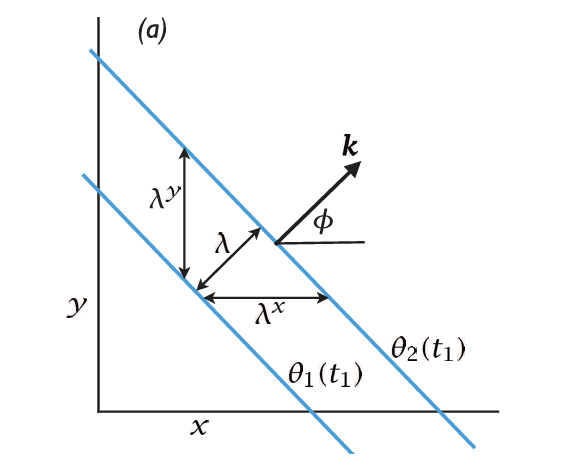
\includegraphics[width=0.5\textwidth,height=\textheight]{figures/plane_wave.png}

}

\caption{\label{fig-plane_wave_crest}Propagation of plane wave crests.}

\end{figure}

Phase speed is the distant that the crests (or troughs) of a wave are
travelling per unit of time. To find the value of phase speed, (at any
instance in time) we align our coordinate along the \(\kb\) axis as
shown in Figure~\ref{fig-plane_wave_crest}. If denote the position along
the \(\kb\) axis in the new coordinate by \(x^*\),
\(\kb \cdot \xb = k x^*\). We then write Equation~\ref{eq-planewave_exp}
as \[
    \psi = A e^{i (\kb . \xb - \omega t)} = A e^{i k (x^*- c t)} ,
\] where \begin{equation}\protect\hypertarget{eq-phase_speed}{}{
    c_p = \frac{\omega}{k}
}\label{eq-phase_speed}\end{equation} is the phase speed. From this form
we can see that the wave function is simply shifted along the \(\kb\)
direction by \(c t\). Hence, if we pick a point on the wave (for example
on a crest), it moves along the \(\kb\) axis with the speed \(c\).

\begin{tcolorbox}[enhanced jigsaw, left=2mm, opacityback=0, coltitle=black, bottomtitle=1mm, title={Example}, toprule=.15mm, colbacktitle=quarto-callout-tip-color!10!white, breakable, arc=.35mm, titlerule=0mm, colback=white, toptitle=1mm, opacitybacktitle=0.6, rightrule=.15mm, bottomrule=.15mm, colframe=quarto-callout-tip-color-frame, leftrule=.75mm]

Based on the definition of phase speed in Equation~\ref{eq-phase_speed},
we derive \(c\) for the following equations
\begin{equation}\protect\hypertarget{eq-PlaneWave_1D}{}{  \frac{\partial \psi}{\partial t} + \alpha \ \frac{\partial \psi}{\partial x} = 0 }\label{eq-PlaneWave_1D}\end{equation}
\begin{equation}\protect\hypertarget{eq-RossbyWave_1D}{}{    \frac{\partial}{\partial t} \frac{\partial^2 \psi}{\partial x^2} \psi + \beta \ \frac{\partial \psi}{\partial x} = 0. }\label{eq-RossbyWave_1D}\end{equation}
We can first derive the dispersion relation for the above systems and
then divide \(\omega\) by \(k\) to get the phase speed. We have already
found the dispersion for Equation~\ref{eq-PlaneWave_1D} in
Equation~\ref{eq-planewave_disprel}. Dividing this expression by \(k\),
we obtain \(c_p = \alpha\). The system Equation~\ref{eq-RossbyWave_1D}
is a one-dimensional case of Equation~\ref{eq-RossbyWave_3D}, where
\(k = k_x\) and \(k_y = k_z =0\). Dividing
Equation~\ref{eq-RossbyWave_disprel} by \(k\) leads to
\(c_p = -\beta / k_x\).

\end{tcolorbox}

It is common to assign a direction to the phase speed and turn it into a
velocity vector. Considering that wave crests propagate along \(\kb\) we
can define the phase velocity as \[
    \boldsymbol{c}_p = \frac{\omega}{k} \ \frac{\kb}{k}.
\] (decide later if you want to talk about phase velocity in more
detail. probably better not to bother)

\begin{figure}

\begin{minipage}[t]{0.50\linewidth}

{\centering 

\raisebox{-\height}{

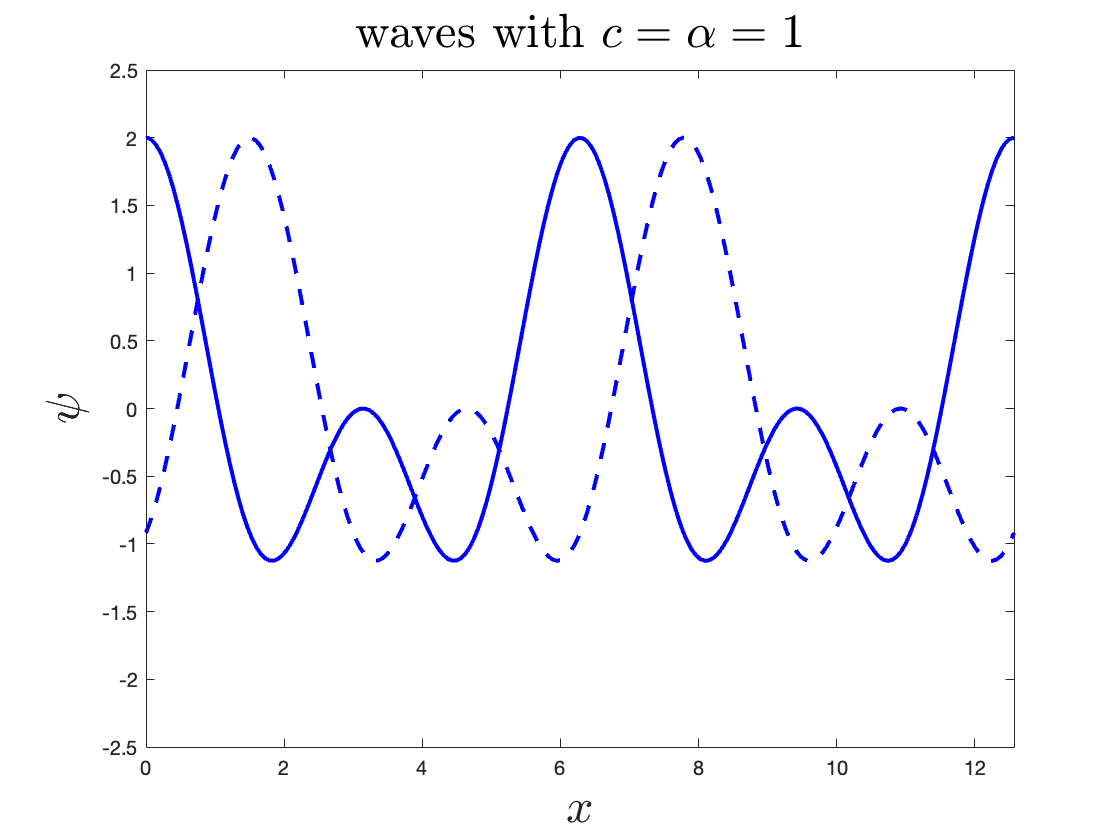
\includegraphics{figures/nondispers2waves.png}

}

}

\end{minipage}%
%
\begin{minipage}[t]{0.50\linewidth}

{\centering 

\raisebox{-\height}{

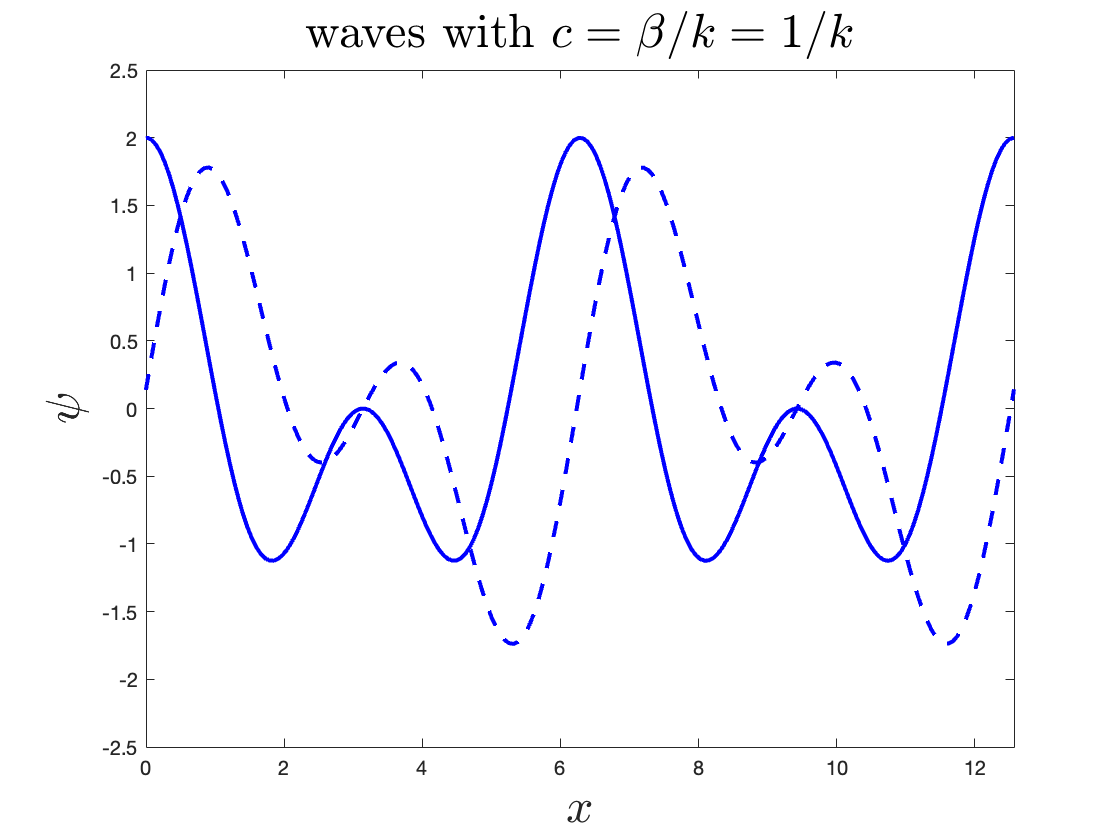
\includegraphics{figures/dispers2waves.png}

}

}

\end{minipage}%

\caption{\label{fig-disp_nondispWave}Propagation of two superimposed
waves: left) non-dispersive and right) dispersive. The solid line is the
initial wave \(\psi(x,t=0)\) and the dashed line after 1.5 time
\(\psi(x,t=1.5)\).}

\end{figure}

Now let's consider a (one-dimensional) compound wave that consists of
two wavenumbers, for example
\begin{equation}\protect\hypertarget{eq-twowaves_1_2}{}{
    \psi = A_1 e^{i ( x - c_1 t)} + A_2 e^{i 2 ( x - c_2 t)}. 
}\label{eq-twowaves_1_2}\end{equation} If this wave evolves under
Equation~\ref{eq-PlaneWave_1D} we find that phase velocity of both
components are the same \(c_1 = c_2 = \alpha\). This means that both
signals (wave components) move at the same speed so the initial shape of
the wave will be preserved in time and just gets shifted along the x
axis. The story is very different for the system
Equation~\ref{eq-RossbyWave_1D} as each component of the wave has a
different velocity \(c_1 = \beta\) and \(c_2 = \beta / 2\). This means
that the shape of the wave deforms in time as its constituents propagate
at different speed. This is demonstrated in figure
Figure~\ref{fig-disp_nondispWave}. The first systems
Equation~\ref{eq-PlaneWave_1D} belongs to a class of waves that are
called \emph{non-dispersive}. For non-dispersive waves the phase speed
does not depend on the wavenumber (left panel of
Figure~\ref{fig-disp_nondispWave}). The second system
Equation~\ref{eq-RossbyWave_1D} is an example of \emph{dispersive} waves
for which the phase speed is an explicit function of wavenumber (right
panel of Figure~\ref{fig-disp_nondispWave}).

\hypertarget{group-velocity}{%
\subsection{Group velocity}\label{group-velocity}}

\begin{figure}

{\centering 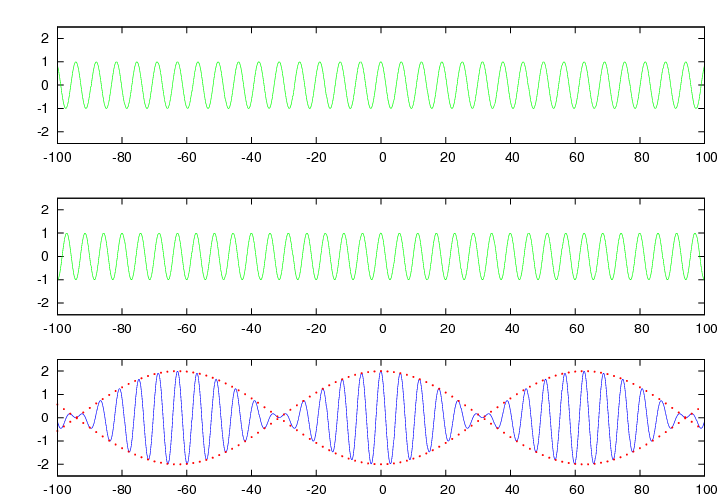
\includegraphics[width=0.65\textwidth,height=\textheight]{figures/Group_Vel.png}

}

\caption{\label{fig-groupvel}The signals of first and second row plots,
with slightly different frequencies are added generating the bottom plot
signal.}

\end{figure}

Energy and information do not necessarily travel at the phase speed. We
do not care too much about how individual crests and troughs propagate
in time. Instead, we want to know how a packet or bundle of them move
together. Their collective motion shows how much energy and information
is transferred by them. The quantity that characterises such a
collective motion is the \emph{group velocity}.

To understand the concept of group velocity, we consider a superposition
of two waves similar to Equation~\ref{eq-twowaves_1_2}
\begin{equation}\protect\hypertarget{eq-twoSimilarWaves}{}{
    \psi = A \left[ e^{i ( k_1 x - \omega_1 t)} + e^{i (k_2 x - \omega_2 t) } \right], 
}\label{eq-twoSimilarWaves}\end{equation} but this time we set the
frequency of individual signals to \(\omega_1 = \omega + \Delta \omega\)
and \(\omega_2 = \omega - \Delta \omega\), and their wavenumbers to
\(k_1 = k + \Delta k\) and \(k_2 = k - \Delta k\). If \(\Delta k\) and
\(\Delta \omega\) are small, these two components will have similar
frequencies and wavenumbers. An example of two wave signals with
slightly different frequencies and wavenumbers is depicted in the top
rows of Figure~\ref{fig-groupvel}. The bottom row of this figure shows
the superposition of these waves, which forms a wave packets (an
envelope of crests and troughs) that look like a wave itself. We can see
this in a mathematical expression by simplifying
Equation~\ref{eq-twoSimilarWaves} \[
    \psi = A e^{i ( k x - \omega t)} \left[ e^{i ( \Delta k x - \Delta \omega t)} + e^{- i ( \Delta k x - \Delta \omega t)}  \right] = A \cos (\Delta k x - \Delta \omega t) e^{i ( k x - \omega t)}   
\] The amplitude of the superposition is no longer constant and instead
is \emph{modulated} by \(\cos(\Delta k x - \Delta \omega t)\). Just like
the original wave signals, this modulated envelope moves in time,
however, with a different speed that is \(\Delta \omega / \Delta k\).
This quantity at the limit of \(\Delta k, \Delta \omega \to 0\) is the
group velocity \(c_g = \partial \omega / \partial k\). Group velocity is
equal to the phase speed only for non-dispersive waves, i.e.~when the
frequency is a linear function of wavenumber. The energy in a wave is
transported by group velocity. To have a better understanding of this
phenomenon, consider the nodes between the envelopes in figure
Figure~\ref{fig-groupvel}. The wave function is zero at these nodes so
the energy cannot be transferred across them. These nodes (as well as
the envelopes between them that contains the wave energy) move with the
group velocity. We can generalise this concept to three dimensions and
define the group velocity as
\begin{equation}\protect\hypertarget{eq-groupVel_def}{}{
    \boldsymbol{c}_g = \nabla_{\kb} \omega = \ddy{\omega}{\kb} = \left(\ddy{\omega}{k_x}, \ddy{\omega}{k_y}, \ddy{\omega}{k_z} \right)
}\label{eq-groupVel_def}\end{equation}

\hypertarget{sec-SW_waves}{%
\section{Poincaré waves in the Shallow Water
equations}\label{sec-SW_waves}}

Now that we are equipped with some basic concepts from wave dynamics, we
can study waves in geophysical flows. One might ask why waves appear so
prominently in large-scale geophysical systems. In the previous chapter
we saw that the leading-order dynamics at large scales
(\(\mathcal{L} \approx \mathcal{L}_d\)) is quasigeostrophic. With a
different timescale, and still at small Rossby number with
\(\mathcal{L} \approx \mathcal{L}_d\), wave dynamics can also emerge. In
this course we demonstrate this for the Shallow Water system; similar
arguments can be made for the Boussinesq equations.

We consider the Shallow Water equations with a flat bottom and place
\(z=0\) at the mean free-surface level. With these assumptions,
\(\eta_b = - H\) and \(h = \eta + H\), where \(H\) is the (constant)
mean depth. Writing the Shallow Water equations in terms of \(\eta\) and
\(\vb\) (substituting \(h = \eta + H\)) gives
\begin{equation}\protect\hypertarget{eq-SWxi}{}{
\begin{aligned}
    \frac{\partial \vb}{\partial t} + (\vb\cdot\gradH)\vb + \fb\times\vb &= -g \ \gradH \eta, \\
    \frac{\partial \eta}{\partial t} + H \ \gradH \cdot \vb  + \gradH \cdot (\eta \vb) &= 0.
\end{aligned}
}\label{eq-SWxi}\end{equation}

This formulation allows us to distinguish the scale of height variations
from the mean depth \(H\). We now non-dimensionalise
Equation~\ref{eq-SWxi} using
\begin{equation}\protect\hypertarget{eq-wavescalingSW}{}{
   (x,y) = {\mathcal{L}}{({x^*},{y^*})}, \quad (u,v) =  {\mathcal{U}}{({u^*},{v^*})}, \quad t = \frac{1}{f_0} t^* , \quad \eta = \frac{f_0\mathcal{L} \ \mathcal{U}}{g} \eta^*, \quad \fb = f_0 \fb^* .
}\label{eq-wavescalingSW}\end{equation}

This is very similar to the scaling we used for geostrophic theory,
except that we now choose the characteristic time scale to be \(1/f_0\)
rather than the advective time scale \(\mathcal{L}/\mathcal{U}\). In
large-scale geophysical flows, \(1/f_0\) is typically shorter than
\(\mathcal{L}/\mathcal{U}\), so we are focusing on dynamics that are
faster than quasigeostrophic motions.

The dimensionless shallow water equations obtained from
Equation~\ref{eq-wavescalingSW} are
\begin{equation}\protect\hypertarget{eq-ndSWxi}{}{
\begin{aligned}
    \frac{\partial \nd{\vb}}{\partial \nd{t}} + \Ro \ (\nd{\vb}\cdot \gradH^*) \nd{\vb} + \nd{\fb} \times \nd{\vb} &= - \ \gradH^* \nd{\eta}, \\
    \frac{\partial \nd{\eta}}{\partial \nd{t}} + \left( \frac{\mathcal{L}_d}{\mathcal{L}} \right)^2 \ \gradH^* \cdot \nd{\vb}  + \Ro \ \gradH^* \cdot (\nd{\eta} \nd{\vb}) &= 0,
\end{aligned}
}\label{eq-ndSWxi}\end{equation} where \(\mathcal{L}_d = \sqrt{gH}/f_0\)
is the deformation radius and \(\Ro = \mathcal{U}/(f_0 \mathcal{L})\) is
the Rossby number.

In the limit of small \(\Ro\) (with
\(\mathcal{L} \approx \mathcal{L}_d\)), these equations simplify to
\begin{equation}\protect\hypertarget{eq-lin-ndSWxi}{}{
\begin{aligned}
    \frac{\partial \nd{\vb}}{\partial \nd{t}} + \nd{\fb} \times \nd{\vb} &= - \ \gradH^* \nd{\eta}, \\
    \frac{\partial \nd{\eta}}{\partial \nd{t}} + \left( \frac{\mathcal{L}_d}{\mathcal{L}} \right)^2 \ \gradH^* \cdot \nd{\vb} &= 0,
\end{aligned}
}\label{eq-lin-ndSWxi}\end{equation} which are simply the linearised
Shallow Water equations. Transforming back to dimensional variables
yields \begin{equation}\protect\hypertarget{eq-linSWxi}{}{
\begin{aligned}
    \frac{\partial \vb}{\partial t} + \fb\times\vb &= -g \ \gradH \eta, \\
    \frac{\partial \eta}{\partial t} + H \ \gradH \cdot \vb &= 0.
\end{aligned}
}\label{eq-linSWxi}\end{equation}

The take-home message from this scaling argument is that, on the fast
timescale \(1/f_0\) and in the limit of small \(\Ro\) with
\(\mathcal{L} \approx \mathcal{L}_d\), the Shallow Water equations
become effectively linear and admit wave solutions.

To derive these wave solutions, it is convenient to introduce \[
    \zeta =  \ddy{v}{x} - \ddy{u}{y}, \qquad
    \delta = \ddy{u}{x} + \ddy{v}{y} = \gradH \cdot \vb,
\] where \(\zeta\) and \(\delta\) are the vertical vorticity and
horizontal divergence, respectively. In other words, we rewrite the
equations in terms of \((\zeta,\delta,\eta)\) instead of \((u,v,\eta)\).

Taking the curl and divergence of Equation~\ref{eq-linSWxi} gives
\begin{equation}\protect\hypertarget{eq-zetdeltSWmom}{}{
\begin{aligned}
    \ddy{\zeta}{t} + f \delta &= 0, \\
    \ddy{\delta}{t} - f \zeta &= -g \gradH^2 \eta.
\end{aligned}
}\label{eq-zetdeltSWmom}\end{equation} Substituting
\(\delta = \gradH \cdot \vb\) into Equation~\ref{eq-linSWxi} gives
\begin{equation}\protect\hypertarget{eq-deltSWheight}{}{
    \frac{\partial \eta}{\partial t} + H \ \delta = 0.
}\label{eq-deltSWheight}\end{equation} Equations
Equation~\ref{eq-zetdeltSWmom} and Equation~\ref{eq-deltSWheight}
together form a closed linear system for \((\zeta,\delta,\eta)\), which
we solve using the wave ansatz \[
    \zeta = \tilde{\zeta}\ e^{i (k_x x + k_y y - \omega t)}, \quad
    \delta = \tilde{\delta}\ e^{i (k_x x + k_y y - \omega t)}, \quad
    \eta = \tilde{\eta}\ e^{i (k_x x + k_y y - \omega t)}.
\] Substituting into
Equation~\ref{eq-zetdeltSWmom}--Equation~\ref{eq-deltSWheight} and
cancelling the exponential factor leads to the matrix system \[
    \begin{bmatrix}
    -i \omega       & f              &  0    \\
    -f              & -i \omega      & - g (k_x^2+k_y^2)    \\
    0               &  H              & -i \omega
    \end{bmatrix} 
    \begin{bmatrix} \tilde{\zeta} \\ \tilde{\delta} \\ \tilde{\eta} \end{bmatrix}
        = 0.
\] The dispersion relation follows from the characteristic equation \[
    -i \omega \bigl(-\omega^2 + gH (k_x^2+k_y^2)\bigr)  + f (-i \omega f ) = 0,
\] which gives \[
  \omega = 0, \qquad \omega = \pm \sqrt{f^2 + g H (k_x^2+k_y^2)}.
\] The non-zero frequencies correspond to shallow-water waves, often
referred to as \emph{Poincaré waves}. For these waves, the phase and
group velocities are \[
    \boldsymbol{c}_p =
    \omega \left(\frac{k_x}{k^2}, \frac{k_y}{k^2}\right) = \frac{\omega}{k^2} \boldsymbol{k}, \qquad
    \boldsymbol{c}_g = \left(\ddy{\omega}{k_x},\ddy{\omega}{k_y}\right) = \left(\frac{gH k_x}{\omega},\frac{gH k_y}{\omega}\right) = \frac{gH}{\omega} \boldsymbol{k}.
\] Thus the phase and group velocities are parallel: wave crests and
wave packets move in the same direction. The ratio of group to phase
speed is \[
    \frac{c_g}{c_p} = \frac{gH}{c_p^2} = \frac{\mathcal{L}^2_d(k_x^2+k_y^2)}{1+\mathcal{L}^2_d(k_x^2+k_y^2)},
\] which shows that wave packets move more slowly than the crests. For
larger wavenumbers (shorter wavelengths), the difference between these
speeds decreases.

\hypertarget{inertia-gravity-waves-in-the-boussinesq-equations}{%
\section{Inertia-gravity waves in the Boussinesq
equations}\label{inertia-gravity-waves-in-the-boussinesq-equations}}

We now consider the wave dynamics in the context of the Boussinesq
system. This leads to an important class of waves in the atmosphere and
ocean: \emph{inertia--gravity waves}. These waves are associated with
two restoring effects introduced earlier: buoyancy and the Coriolis
force. They can be generated in many ways, e.g.~atmospheric flows
impinging on topography, tides in the ocean, or wind forcing at the sea
surface. Despite their diverse generation mechanisms, the waves that
propagate in the ocean and atmosphere interior follow similar physical
principles.

We can follow a similar scaling argument as in Section
Section~\ref{sec-SW_waves} to justify linearising the Boussinesq
equations for the fast-timescale motion. We can also consider small
disturbances propagating in a fluid initially at rest. If the
disturbances are small, we can neglect the quadratic nonlinear terms,
leading to the linearised equations. In the hydrostatic Boussinesq
approximation, the linear equations are
\begin{equation}\protect\hypertarget{eq-lin-Bous}{}{
\begin{aligned}
\frac{\partial \vb}{\partial t} + \fb \times \vb &= - \frac{1}{\rho_0} \ \gradH p, \\
b &= \frac{1}{\rho_0} \frac{\partial p }{\partial z}, \\
\gradH \cdot \vb + \frac{\partial w}{\partial z} &= 0, \\
\frac{\partial b}{\partial t} + N^2 w &= 0,
\end{aligned}
}\label{eq-lin-Bous}\end{equation} where \(b\) is buoyancy, \(N\) the
buoyancy frequency, and \(w\) the vertical velocity.

Using a plane-wave ansatz for all variables, \[
    u = \tilde{u}\ e^{i (\kb \cdot \xb - \omega t)}, \quad v = \tilde{v}\ e^{i (\kb \cdot \xb - \omega t)}, \quad w = \tilde{w}\ e^{i (\kb \cdot \xb - \omega t)},
\] \[
    b = \tilde{b}\ e^{i (\kb \cdot \xb - \omega t)}, \quad p = \tilde{p}\ e^{i (\kb \cdot \xb - \omega t)},
\] and substituting into Equation~\ref{eq-lin-Bous}, then cancelling the
common factor \(e^{i (\kb \cdot \xb - \omega t)}\), we obtain
\begin{equation}\protect\hypertarget{eq-klin-Bous}{}{
\begin{aligned}
-i\omega \tilde{u} -f \tilde{v} &= -\frac{1}{\rho_0} \ i k_x \tilde{p}, \\
-i\omega \tilde{v} +f \tilde{u} &= -\frac{1}{\rho_0} \ i k_y \tilde{p}, \\
\tilde{b} &= \frac{1}{\rho_0} \ i k_z \tilde{p}, \\
i k_x \tilde{u} + i k_y \tilde{v} +  i k_z \tilde{w} &= 0, \\
-i \omega \tilde{b} + N^2 \tilde{w} &= 0.
\end{aligned}
}\label{eq-klin-Bous}\end{equation}

We eliminate \(\tilde{p}\) from the first two equations using the third,
and eliminate \(\tilde{w}\) from the last using the fourth, to obtain
the reduced system \[
    \begin{bmatrix}
    -i \omega       & -f                & k_x / k_z    \\
    f               & -i \omega         & k_y / k_z    \\
    - N^2 k_x/k_z   & - N^2 k_y/k_z     & -i \omega
    \end{bmatrix} 
    \begin{bmatrix} \tilde{u} \\ \tilde{v} \\ \tilde{b} \end{bmatrix}
        = 0.
\] The dispersion relation follows from the characteristic equation of
this matrix: \[
    i \omega \left(-\omega^2 + f^2 + N^2 \frac{k_x^2+k_y^2}{k_z^2}\right) = 0,
\] so \begin{equation}\protect\hypertarget{eq-IGWdispersion}{}{
  \omega = 0, \qquad \omega = \pm \sqrt{f^2 + N^2 \frac{k_h^2}{k_z^2}},
}\label{eq-IGWdispersion}\end{equation} where
\(k_h = \sqrt{k_x^2+k_y^2}\). We focus on the non-zero frequencies,
which describe propagating waves.

The dispersion relation Equation~\ref{eq-IGWdispersion} reveals key
features of inertia--gravity waves. The frequency for a given wavevector
\(\kb\) depends only on the ratio \(k_h/k_z\). As illustrated
schematically in Figure Figure~\ref{fig-IGWcone}, this ratio is equal to
\(\tan\theta\), where \(\theta\) is the angle between the wavevector and
the vertical, so \[
    \frac{k_h}{k_z} = \tan(\theta).
\] Thus, all wavevectors with the same \(\theta\) have the same
frequency. Surfaces of constant frequency in wavenumber space are
therefore double cones (Figure Figure~\ref{fig-IGWcone}).

\begin{figure}

{\centering 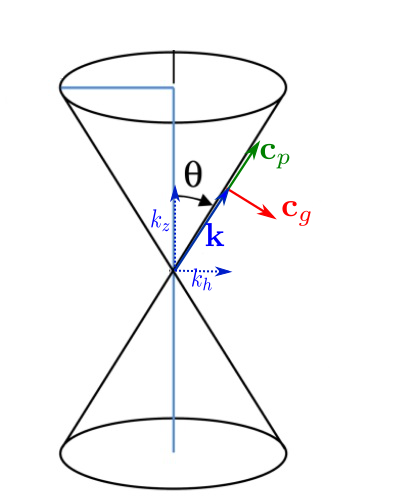
\includegraphics[width=0.35\textwidth,height=\textheight]{figures/coneTheta.png}

}

\caption{\label{fig-IGWcone}Cone of constant frequency for
inertia-gravity waves with their group and phase velocity.}

\end{figure}

From the definition of group velocity Equation~\ref{eq-groupVel_def}, we
know that \(\boldsymbol{c}_g\) is perpendicular to surfaces of constant
\(\omega\), so it is normal to these cones. The phase velocity, on the
other hand, is parallel to \(\kb\) and thus lies along the cone. As a
result, the group and phase velocities are perpendicular to one another:
energy and information propagate in a direction perpendicular to the
propagation of individual crests.

We can see this explicitly by differentiating
Equation~\ref{eq-IGWdispersion} with respect to \(\kb\):
\begin{equation}\protect\hypertarget{eq-hydstat-IGWdisp}{}{
    \boldsymbol{c}_g =
    \left( \frac{N^2  k_x/ k_z^2}{\omega}, \frac{N^2 k_y/k_z^2}{\omega},  - \frac{N^2 k_h^2/k_z^3}{\omega} \right).
}\label{eq-hydstat-IGWdisp}\end{equation} It is straightforward to check
that the inner product of this vector with \(\kb = (k_x, k_y, k_z)\) is
zero, confirming that \(\boldsymbol{c}_g \perp \kb\).

We can repeat the analysis for the non-hydrostatic Boussinesq equations
(see the earlier Boussinesq chapter) to obtain the dispersion relation
\begin{equation}\protect\hypertarget{eq-nonhydstat-IGWdisp}{}{
    \omega = \pm \sqrt{f^2 \frac{k_z^2}{k^2} + N^2 \frac{k_h^2}{k^2}} = \pm \sqrt{f^2 \cos^2(\theta) + N^2 \sin^2(\theta)},
}\label{eq-nonhydstat-IGWdisp}\end{equation} where again \(\theta\) is
the angle from the vertical.

The hydrostatic and non-hydrostatic dispersion relations share a key
feature: both depend only on \(\theta\), so the constant-frequency
surfaces are the same cones, and \(\boldsymbol{c}_p\) and
\(\boldsymbol{c}_g\) remain perpendicular. The non-hydrostatic
dispersion relation Equation~\ref{eq-nonhydstat-IGWdisp}, however, shows
an additional property: the wave frequency is bounded between \(f\) and
\(N\) (for typical geophysical conditions with \(N > f\)). This is
consistent with observations in the atmosphere and ocean.

\hypertarget{rossby-waves}{%
\section{Rossby waves}\label{rossby-waves}}

\begin{figure}

{\centering 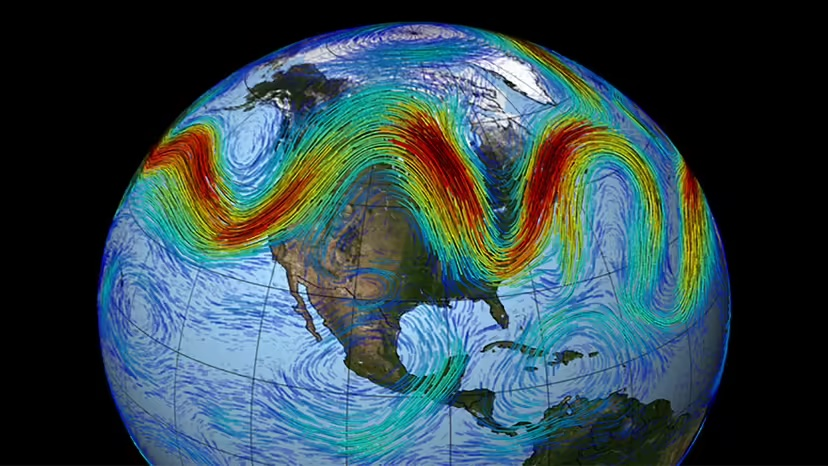
\includegraphics[width=0.65\textwidth,height=\textheight]{figures/RossbyWave.jpeg}

}

\caption{\label{fig-RossbyWaveSim}Rossby waves interacting with the jet
stream. Figure adapted from an animation by NASA's Goddard Space Flight
Center.}

\end{figure}

Rossby waves are another important class of waves in the ocean and
atmosphere. They have relatively large spatial scales---comparable to
the planetary radius---and are therefore also called \emph{planetary
waves}. Figure Figure~\ref{fig-RossbyWaveSim} illustrates the large
scale of atmospheric Rossby waves. These waves play a crucial role in
shaping weather patterns, as they can transport substantial masses of
air or water and give rise to cyclones and anticyclones.

The restoring mechanism for Rossby waves is the variation of the
Coriolis parameter with latitude, the so-called \(\beta\)-effect
introduced in the earlier chapter on the tangent-plane approximation. As
usual, we will start from a set of linear equations and derive a
dispersion relation. For Rossby waves we begin from the quasigeostrophic
(QG) potential vorticity equation
\begin{equation}\protect\hypertarget{eq-QGrepeat}{}{
     \frac{D q}{D t}  = 0,
}\label{eq-QGrepeat}\end{equation} where \(q\) is the potential
vorticity (PV). We did not start from the full Boussinesq equations,
because at large scales the QG approximation is appropriate. As
discussed in previous chapters, PV conservation holds for both the
shallow-water and Boussinesq systems, but the expressions for \(q\)
differ. Starting from Equation~\ref{eq-QGrepeat}, one can derive Rossby
waves in both systems; here we restrict attention to the shallow-water
case for simplicity, noting that many properties are shared.

Recall that the QG PV for the shallow-water system is
\begin{equation}\protect\hypertarget{eq-PVSWrepeat}{}{
    q = \gradH^2 \psi + f_0 + \beta y -\frac{1}{\mathcal{L}_d^2} \psi,
}\label{eq-PVSWrepeat}\end{equation} where
\(\mathcal{L}_d = \sqrt{g H}/f_0\) is the deformation radius.

We linearise Equation~\ref{eq-QGrepeat} about a time-independent basic
state. Unlike the inertia--gravity wave case, the basic state now
includes a non-zero flow. We assume a uniform zonal (east--west) basic
flow, appropriate for the strong zonal jets often observed in
large-scale atmospheric and oceanic flows. We decompose the flow into a
zonal mean (denoted by an overbar) and a perturbation (denoted by a
prime): \[
    \psi = \overline{\psi}(y) + \psi'(x,y,t) = - \overline{u}\, y + \psi'(x,y,t),
\] \begin{equation}\protect\hypertarget{eq-velRoWave}{}{
    u = \overline{u} - \frac{\partial \psi'}{\partial y}, \quad v = \frac{\partial \psi'}{\partial x},
}\label{eq-velRoWave}\end{equation} where \(\overline{u}\) is a constant
zonal velocity and we have used \(\overline{v} = 0\). The PV
Equation~\ref{eq-PVSWrepeat} becomes
\begin{equation}\protect\hypertarget{eq-qRoWave}{}{
    q = \gradH^2 \psi' + f_0 + \beta y + \frac{\overline{u} y}{\mathcal{L}_d^2} -\frac{\psi'}{\mathcal{L}_d^2}.
}\label{eq-qRoWave}\end{equation} Substituting
Equation~\ref{eq-velRoWave} and Equation~\ref{eq-qRoWave} into
Equation~\ref{eq-QGrepeat} and simplifying yields \[
    \ddy{}{t}\left( \gradH^2 \psi' -\frac{\psi'}{\mathcal{L}_d^2} \right) 
    + \left( \overline{u} - \frac{\partial \psi'}{\partial y} \right) \ddy{}{x} \left( \gradH^2 \psi' -\frac{\psi'}{\mathcal{L}_d^2} \right) +
    \frac{\partial \psi'}{\partial x} \ddy{}{y} \left( \gradH^2 \psi' + \beta y + \frac{\overline{u} y}{\mathcal{L}_d^2} -\frac{\psi'}{\mathcal{L}_d^2} \right) = 0.
\] Neglecting products of perturbation quantities (as usual in
linearisation) gives \[
   \left(\ddy{}{t} + \overline{u} \ddy{}{x}\right) \left( \gradH^2 \psi' -\frac{\psi'}{\mathcal{L}_d^2} \right) 
   + \frac{\partial \psi'}{\partial x} \left( \beta + \frac{\overline{u}}{\mathcal{L}_d^2} \right) = 0.
\] Substituting the wave ansatz
\(\psi' = \tilde{\psi} e^{i ( k_x x + k_y y - \omega t)}\) in the above
equation, we derive the dispersion relation \[
    \omega = \overline{u} k_x - k_x \frac{\beta + \overline{u}/\mathcal{L}_d^2}{k_x^2+k_y^2+1/\mathcal{L}_d^2}.
\] It is instructive to consider the special case of a very large
deformation radius, \(\mathcal{L}_d \to \infty\), which is a good
approximation when the horizontal scale of the motion is much smaller
than \(\mathcal{L}_d\). In this limit, the dispersion relation reduces
to \[
    \omega = \overline{u} k_x - \frac{\beta k_x }{k_x^2+k_y^2}.
\] The (scalar) phase speed in the \(x\)-direction is then
\begin{equation}\protect\hypertarget{eq-cp-RossWav-Inf}{}{
    c_{p,x} = \frac{\omega}{k_x} = \overline{u} - \frac{\beta}{k_x^2+k_y^2}.
}\label{eq-cp-RossWav-Inf}\end{equation}

\begin{tcolorbox}[enhanced jigsaw, toprule=.15mm, left=2mm, opacityback=0, breakable, arc=.35mm, colback=white, rightrule=.15mm, bottomrule=.15mm, colframe=quarto-callout-note-color-frame, leftrule=.75mm]
\begin{minipage}[t]{5.5mm}
\textcolor{quarto-callout-note-color}{\faInfo}
\end{minipage}%
\begin{minipage}[t]{\textwidth - 5.5mm}

In the absence of a mean flow (\(\overline{u} = 0\)), the phase speed in
the \(x\)-direction is negative for all wavenumbers, meaning that Rossby
waves propagate westward. If we choose an eastward background flow with
\(\overline{u} = \beta / (k_x^2+k_y^2)\), the phase speed becomes zero
and the Rossby wave pattern is stationary.

\end{minipage}%
\end{tcolorbox}

The group velocity of Rossby waves in the limit
\(\mathcal{L}_d \to \infty\) is
\begin{equation}\protect\hypertarget{eq-cg-RossWav-Inf}{}{
    \boldsymbol{c}_g = \left(\ddy{\omega}{k_x} ,\ddy{\omega}{k_y} \right) = \left( \overline{u} + \frac{\beta(k_x^2-k_y^2)}{(k_x^2+k_y^2)^2}, \frac{2 k_x k_y \beta}{(k_x^2+k_y^2)^2}\right).
}\label{eq-cg-RossWav-Inf}\end{equation} Unlike inertia--gravity waves,
the phase and group velocities for Rossby waves are not perpendicular;
instead, the angle between them depends on the wavenumber and the
background flow.

Comparing Equation~\ref{eq-cp-RossWav-Inf} and
Equation~\ref{eq-cg-RossWav-Inf}, we find that the \(x\)-component of
the group velocity can be written as the \(x\)-component of the phase
velocity plus a positive correction: \[
    \boldsymbol{c}_g \cdot \eb_x = \boldsymbol{c}_p \cdot \eb_x + \frac{2 k_x^2 \beta}{(k_x^2+k_y^2)^2}.
\] This is an interesting result: the group velocity of the Rossby wave
is shifted eastward relative to its phase velocity. For example,
consider a stationary Rossby wave (with \(\mathcal{L}_d \to \infty\) and
\(\omega = 0\)). Although the wave pattern is fixed in space, the
corresponding wave packets transport energy and mass eastward.

\begin{figure}

{\centering 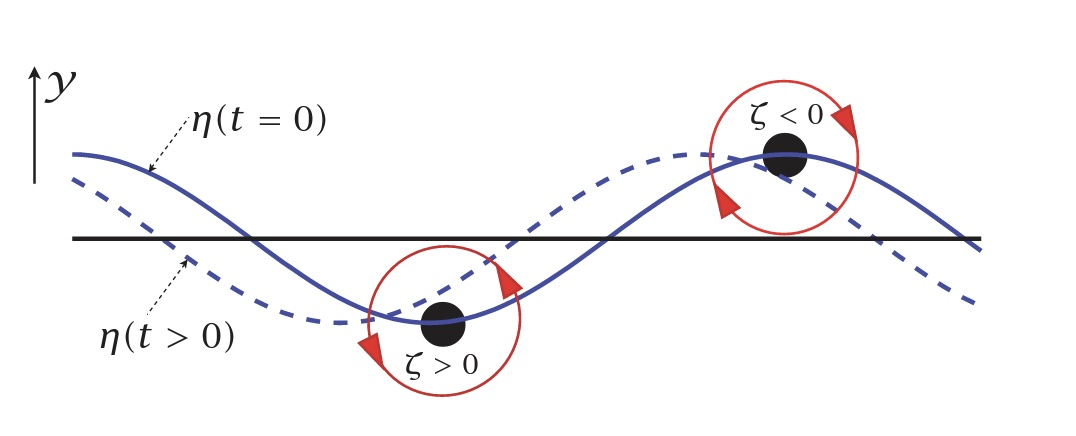
\includegraphics[width=0.65\textwidth,height=\textheight]{figures/RossbyWaveSchem.jpg}

}

\caption{Mechanism of a Rossby wave with infinite deformation radius. An
initial disturbance displaces a material line at constant latitude
(black straight line) into the solid curve \(\eta(t=0)\). Conservation
of absolute vorticity (\(\zeta + f_0 + \beta y\)) leads to the
production of relative vorticity \(\zeta\) for parcels moved northward
or southward. The induced velocity field (arrows) then advects the fluid
parcels further, and the material line evolves into the dashed curve
\(\eta(t>0)\), with the phase propagating westward.}

\end{figure}

We can gain more physical intuition for Rossby waves (with large
deformation radius) using a heuristic argument. Consider a line of fluid
parcels at a fixed latitude \(y\), represented by the black straight
line in Figure @fig:Mechanism\_RossbyWave. Suppose this material line is
disturbed so that it acquires the shape \(\eta(t=0)\) (solid blue
curve).

The PV in the limit \(\mathcal{L}_d \to \infty\) becomes
\(q = \zeta + f_0 + \beta y\) and is conserved according to
Equation~\ref{eq-QGrepeat}. A parcel displaced northward (to larger
\(y\)) must therefore acquire negative relative vorticity (\(\zeta<0\))
to keep its absolute vorticity unchanged; a parcel displaced southward
must acquire positive vorticity. As indicated in Figure
@fig:Mechanism\_RossbyWave, these vorticity anomalies induce a velocity
field that pushes the neighbouring parcels westward, causing the
disturbed material line (solid curve) to evolve into the dashed curve
\(\eta(t>0)\). Thus the disturbance propagates westward, consistent with
the sign of the \(x\)-component of the phase velocity in
Equation~\ref{eq-cp-RossWav-Inf} when \(\overline{u}=0\).

\hypertarget{chap-turbulence}{%
\chapter{Turbulence in geophysical flows}\label{chap-turbulence}}

\hypertarget{introduction-1}{%
\section{Introduction}\label{introduction-1}}

\begin{figure}

{\centering 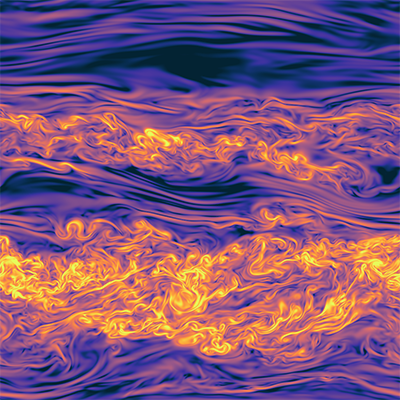
\includegraphics{figures/turbulent_mixing.png}

}

\caption{\label{fig-mixingturbulence}Mixing in the flow by turbulence.}

\end{figure}

\begin{quote}
\emph{I am an old man now, and when I die and go to heaven, there are
two matters on which I hope for enlightenment. One is quantum
electrodynamics and the other is the turbulent motion of fluids. About
the former, I am really rather optimistic.}
\end{quote}

\begin{quote}
\emph{There is a physical problem that is common to many fields, that is
very old, and that has not been solved. It is not the problem of finding
new fundamental particles, but something left over from a long time
ago---over a hundred years. Nobody in physics has really been able to
analyze it mathematically satisfactorily, in spite of its importance to
the sister sciences. It is the analysis of circulating or turbulent
fluids.}
\end{quote}

The latter quotation is attributed to Richard
Feynman,\footnote{From *The Feynman Lectures on Physics*, Vol.~1; .} one
of the most celebrated physicists of the twentieth century, while the
former originates from Sir Horace Lamb nearly a century earlier. These
and similar remarks frequently appear in opening paragraphs of talks,
articles, and books on turbulence---not as a celebration of progress,
but as an acknowledgement of the persistent challenges this subject
poses. Beyond their wit, they reflect the inherent difficulty of
turbulence in physics, a difficulty that begins with the challenge of
defining it.

Before attempting such a definition, let us recall an important
dimensionless quantity that is central to the study of turbulence: the
\textbf{Reynolds number}
\begin{equation}\protect\hypertarget{eq-defRe}{}{
\mathrm{Re} = \frac{\mathcal{U}\mathcal{L}}{\nu},
}\label{eq-defRe}\end{equation} where \(\mathcal{U}\) is a
characteristic velocity scale, \(\mathcal{L}\) a characteristic length
scale, and \(\nu\) the kinematic viscosity. The inverse of
\(\mathcal{U}/\nu\) has units of length and represents a scale at which
molecular viscosity becomes significant---one of the smallest
dynamically relevant length scales in the flow. By contrast, the scale
\(\mathcal{L}\) typically denotes the largest dynamically active scales,
such as the forcing scale, domain size, or the scale of the most
energetic vortices. The Reynolds number therefore quantifies the ratio
between the largest and smallest active spatial scales. Atmospheric and
oceanic flows exhibit enormously large Reynolds numbers (often of order
\(10^{11}\)), reflecting the breadth of scales they involve and the
complexity of their dynamics.

As leading turbulence textbooks acknowledge, any precise definition of
turbulence is at best difficult and arguably impossible. Following their
approach, we characterise turbulence through its principal features:

\textbf{Randomness and chaos:} Turbulent motion is highly irregular and
unpredictable. A hallmark of chaotic systems is the sensitivity to
initial conditions: arbitrarily small perturbations may evolve into
drastically different states. Consequently, deterministic prediction of
particle trajectories or instantaneous field values (e.g.~velocity or
pressure) is infeasible. Instead, turbulence is studied statistically.
Remarkably, despite the apparent randomness, turbulent flows exhibit
universal statistical properties; several of these are explored below.

\textbf{Enhanced mixing and diffusivity:} Turbulence greatly increases
the transport of momentum, heat, and scalar quantities. One may imagine
turbulence as an ``idealised whisk'\,' stirring velocity, temperature,
and other fields, thereby enhancing fluxes and accelerating mixing.

\textbf{A wide range of spatial scales:} Turbulence excites a continuum
of Fourier modes. A flow with only a small number of active modes is not
turbulent, even if chaotic. Because \(\mathrm{Re}\) is (in a loose
sense) the ratio of the outer to inner scales, large Reynolds numbers
are associated with a wide spectral range. In this sense,
``turbulence'\,' is inherently a large--Reynolds-number phenomenon.

\textbf{Nonlinear interactions:} Without nonlinear terms, Fourier modes
evolve independently. The Navier--Stokes equations, however, contain
quadratic nonlinearities. Turbulence requires these nonlinear
interactions to be dynamically significant, allowing energy and other
invariants to be transferred between scales.

In the atmosphere and ocean, the largest scales exceed the dissipation
scale by many orders of magnitude. Between them lies a vast range of
intermediate scales that interact nonlinearly. This richness underpins
both the complexity of weather and the limits of weather predictability.
Thus, it is fair to state that both the atmosphere and ocean are
turbulent systems, although the form and regime of turbulence vary
across spatial and temporal scales.

Before describing specific turbulence regimes in geophysical flows, we
first review a central mathematical tool: the \emph{Fourier transform}.

\hypertarget{fourier-transform}{%
\section{Fourier transform}\label{fourier-transform}}

Because turbulence involves nonlinear energy exchange between scales,
the Fourier transform plays a central role. The Fourier transform of a
function \(f(\xb)\), denoted \(\hat{f}\) or \(\mathcal{F}[f]\), is
defined as \begin{equation}\protect\hypertarget{eq-defFourTrans}{}{
\hat{f}(\kb) = \mathcal{F}[f(\xb)](\kb)
= \int_{-\infty}^{\infty} f(\xb)\, e^{-i\kb\cdot\xb}\, d\xb,
}\label{eq-defFourTrans}\end{equation} where \(\kb = (k_x,k_y,k_z)\) is
the wavevector. The inverse transform is \[
f(\xb) = \mathcal{F}^{-1}[\hat{f}(\kb)](\xb)
= \frac{1}{(2\pi)^3}\int_{-\infty}^{\infty} \hat{f}(\kb)\, e^{i\kb\cdot\xb}\, d\kb.
\]

We frequently use two key properties:

\emph{Linearity:} \[
\mathcal{F}[a f + b g] = a\,\mathcal{F}[f] + b\,\mathcal{F}[g].
\]

\emph{Differentiation:} \[
\mathcal{F}\!\left[\frac{\partial f}{\partial x}\right] = i k_x \hat{f}, \qquad
\mathcal{F}\!\left[\frac{\partial f}{\partial y}\right] = i k_y \hat{f}, \qquad
\mathcal{F}\!\left[\frac{\partial f}{\partial z}\right] = i k_z \hat{f}.
\]

These properties make Fourier space a natural setting in which to
analyse turbulence and energy transfers across scales.

\hypertarget{sec-3Dturb}{%
\section{Theory of 3D isotropic turbulence}\label{sec-3Dturb}}

The modern theory of isotropic turbulence centres on the transfer of
energy from large to small vortices---a process called the \emph{energy
cascade}. Richardson encapsulated this idea in his well-known verse:

\begin{quote}
\emph{Big whirls have little whirls that feed on their velocity,}\\
\emph{and little whirls have lesser whirls and so on to viscosity.}
\end{quote}

Large eddies transfer energy to somewhat smaller eddies, which transfer
it to still smaller eddies, and so on, until the energy reaches
sufficiently small scales that it is dissipated by viscosity. This is
illustrated schematically in the left panel of
Figure~\ref{fig-cascades3D}.

\begin{figure}

\begin{minipage}[t]{0.50\linewidth}

{\centering 

\raisebox{-\height}{

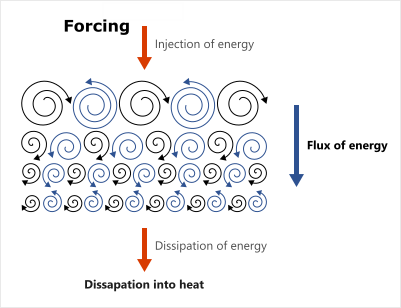
\includegraphics{figures/cascade_schematic.png}

}

}

\end{minipage}%
%
\begin{minipage}[t]{0.50\linewidth}

{\centering 

\raisebox{-\height}{

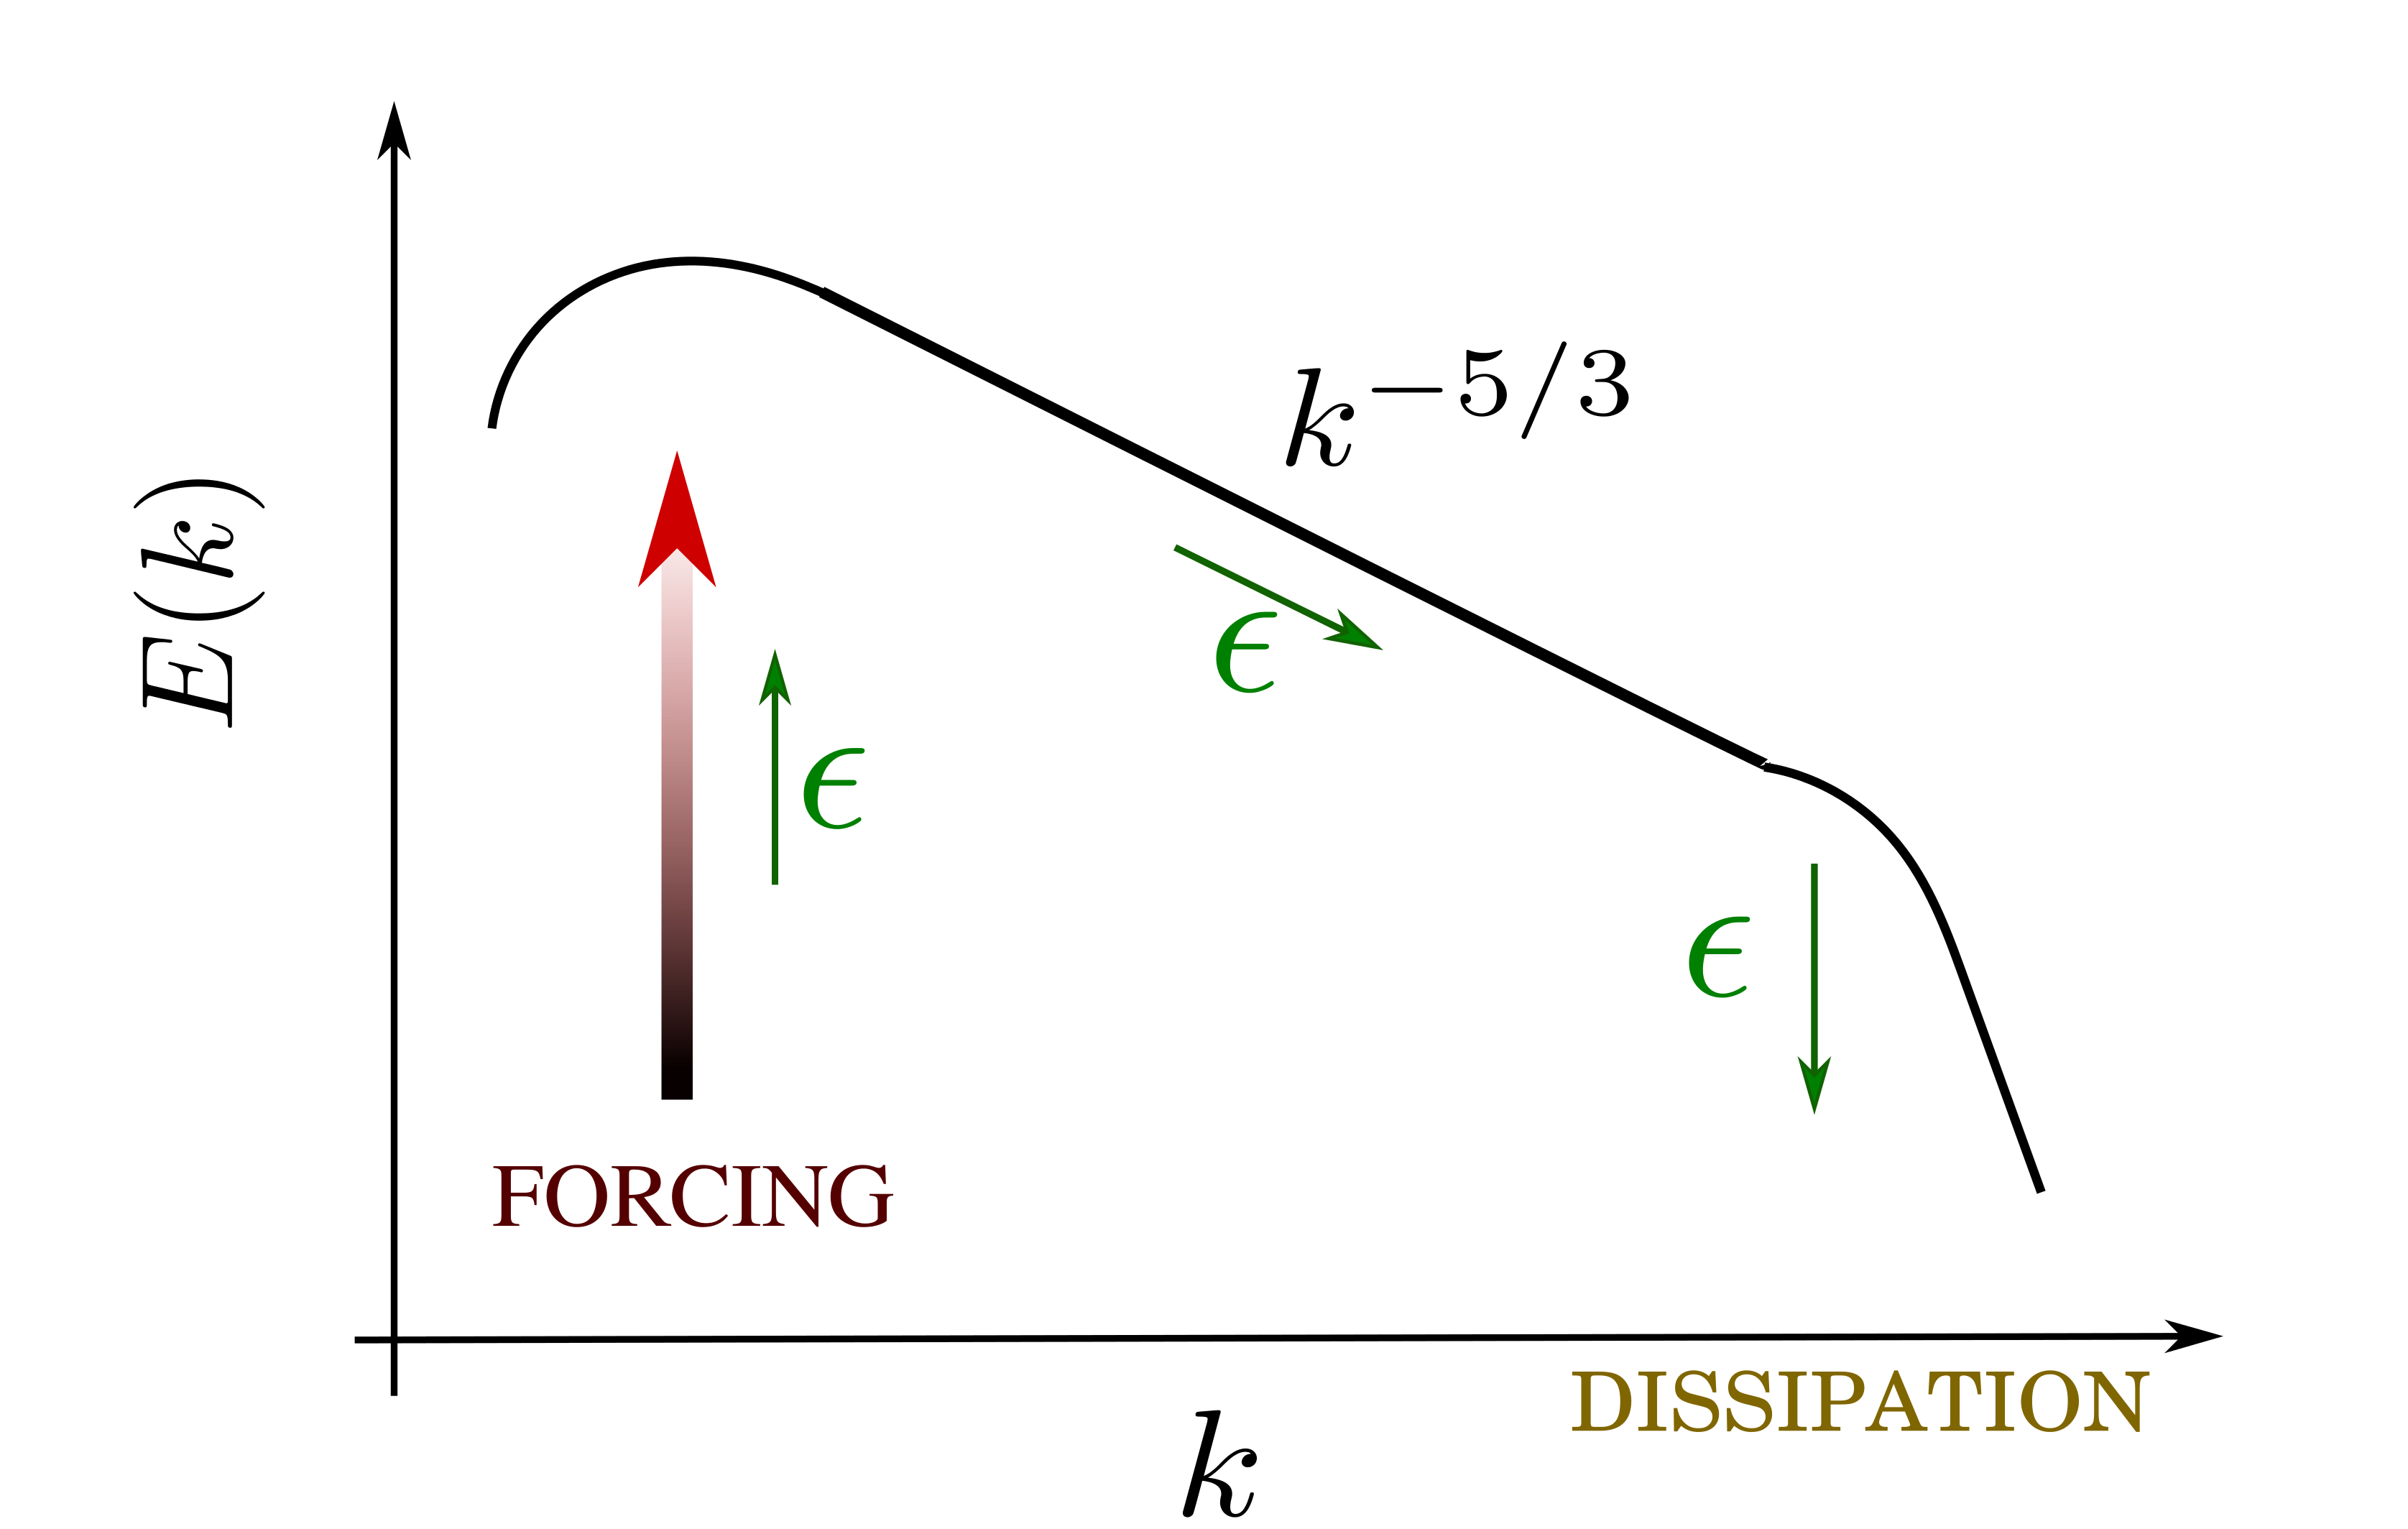
\includegraphics{figures/turbulence3Dcascade.png}

}

}

\end{minipage}%

\caption{\label{fig-cascades3D}Left: schematic picture of energy cascade
by vortices of different sizes. Right: the energy spectrum of isotropic
3D turbulence.}

\end{figure}

Building on this idea, Kolmogorov introduced a phenomenological theory
predicting how energy is distributed across scales. His theory---often
considered the most significant single contribution to
turbulence---applies directly to small-scale atmospheric and oceanic
motions and forms the basis for several geophysical turbulence theories.

Kolmogorov's theory relies on four principal assumptions: (i)
\emph{isotropy}, (ii) \emph{homogeneity}, (iii) \emph{large Reynolds
number}, and (iv) \emph{locality of energy transfer}. Isotropy means
that the statistical properties of the flow are invariant under
rotations of the coordinate system; homogeneity means translation
invariance. These assumptions hold away from boundaries or when boundary
layers are thin relative to the domain.

To describe the distribution of energy among Fourier modes, let
\(\hat{\ub}(\kb)\) be the Fourier transform of the velocity field. The
modal kinetic energy at wavenumber \(\kb\) is \[
\mathcal{E}(\kb) = \frac12\,\hat{\ub}(\kb)\cdot\hat{\ub}(\kb)^*,
\] and Parseval's theorem yields
\begin{equation}\protect\hypertarget{eq-relateEmodalEreal}{}{
E_{\text{tot}}
= \frac{1}{\mathtt{V}}\int_{\mathtt{V}} \frac12\,\ub(\xb)\cdot\ub(\xb)\, d\xb
= \int \mathcal{E}(\kb)\, d\kb.
}\label{eq-relateEmodalEreal}\end{equation}

Isotropy implies that modes with equal \(|\kb|=k\) have statistically
identical energies. This motivates the definition of the \emph{energy
spectrum} \begin{equation}\protect\hypertarget{eq-defEspc}{}{
E(k) = \oint_{S_k} \mathcal{E}(\kb)\, d\mathbf{s},
}\label{eq-defEspc}\end{equation} where \(S_k\) is the sphere of radius
\(k\) in Fourier space. Therefore,
\begin{equation}\protect\hypertarget{eq-relateEavrtoEspc}{}{
E_{\text{tot}} = \int_0^\infty E(k)\, dk.
}\label{eq-relateEavrtoEspc}\end{equation} Thus \(E(k)\,dk\) represents
the kinetic energy per unit mass contained in wavenumbers between \(k\)
and \(k+dk\).

If the flow is statistically stationary, energy conservation dictates
that the rate at which energy is injected into the flow, \(\epsilon\),
must equal the rate at which it is dissipated by viscosity. The energy
spectrum may depend on several quantities, including the forcing \(F\),
the dissipation \(\nu\), the energy flux across each wavenumber
\(\epsilon\), and the wavenumber \(k\):
\begin{equation}\protect\hypertarget{eq-Efun}{}{
E = f(F,\epsilon,k,\nu).
}\label{eq-Efun}\end{equation}

Kolmogorov's final two assumptions now enter. Locality asserts that
energy is transferred mainly between modes of comparable wavenumber.
Because forcing acts at large scales and viscosity at small scales, a
wide inertial subrange exists where neither forcing nor dissipation acts
directly. In this range the spectrum cannot depend on \(F\) or \(\nu\),
leaving \begin{equation}\protect\hypertarget{eq-EfunInertialRange}{}{
E = f_i(\epsilon,k).
}\label{eq-EfunInertialRange}\end{equation}

Dimensional analysis then suggests the form
\begin{equation}\protect\hypertarget{eq-fatch}{}{
E = C\,\epsilon^{\,m}\,k^{\,n},
}\label{eq-fatch}\end{equation} where \(C\) is a dimensionless constant.
With dimensions \[
[E]=L^3T^{-2},\qquad
[\epsilon]=L^2T^{-3},\qquad
[k]=L^{-1},
\] matching powers of \(L\) and \(T\) yields \(m=2/3\) and \(n=-5/3\),
giving the celebrated Kolmogorov spectrum,
\begin{equation}\protect\hypertarget{eq-K41}{}{
E(k) = C\,\epsilon^{2/3} k^{-5/3}.
}\label{eq-K41}\end{equation}

This \(k^{-5/3}\) law describes the energy spectrum of any (sufficiently
isotropic) turbulent flow, regardless of the underlying fluid or
environment. Laboratory experiments and oceanic observations have
verified this law. The right panel of Figure~\ref{fig-cascades3D} shows
the typical 3D isotropic turbulent spectrum.

\hypertarget{sec-2Dturb}{%
\section{2D turbulence}\label{sec-2Dturb}}

While neither the atmosphere nor the ocean is exactly two-dimensional,
the theory of 2D turbulence forms the conceptual foundation of
geostrophic turbulence, which successfully describes many large-scale
geophysical statistics. This connection arises because quasi-geostrophic
(QG) flows and strictly 2D flows share important invariants and exhibit
qualitatively similar nonlinear behaviour.

Consider the 2D incompressible Navier--Stokes equations without
rotation, viscosity, or external forcing:
\begin{equation}\protect\hypertarget{eq-2DNavSto}{}{
\begin{aligned}
\frac{\partial\vb}{\partial t} + (\vb\cdot\nabla)\vb &= -\frac{1}{\rho}\nabla_H p, \\
\nabla\cdot\vb &= 0.
\end{aligned}
}\label{eq-2DNavSto}\end{equation}

Taking the curl yields the vorticity equation
\begin{equation}\protect\hypertarget{eq-EvolVertVort2D}{}{
\frac{D\zeta}{Dt} = 0,
}\label{eq-EvolVertVort2D}\end{equation} where \(\zeta\) is the vertical
vorticity.

A fundamentally different phenomenology emerges in 2D turbulence due to
the conservation of vorticity alongside energy. If vorticity \(\zeta\)
is conserved for each fluid particle, the volume-averaged
\emph{enstrophy}, defined as
\begin{equation}\protect\hypertarget{eq-defZ}{}{
Z_{\text{tot}} =  \frac{1}{\mathtt{V}}\int_{\mathtt{V}} \frac12\,\zeta(\xb)\, \zeta(\xb)\, d\xb
= \frac{1}{2} \int  \hat{\zeta}(\mathbf{k}) \, \hat{\zeta}(\mathbf{k})^* d \mathbf{k},
}\label{eq-defZ}\end{equation} is also conserved. Here, \(\hat{\zeta}\)
denotes the Fourier transform of \(\zeta\).

Analogous to the energy spectrum defined in Equation~\ref{eq-defEspc},
the enstrophy spectrum is given by
\begin{equation}\protect\hypertarget{eq-defZspc}{}{
Z(k) =\frac{1}{2} \int\limits_{S_k} \hat{\zeta}(\mathbf{k}) \hat{\zeta}(\mathbf{k})^* d \mathbf{s},
}\label{eq-defZspc}\end{equation} where \(S_k\) represents circles of
constant \(k\). The enstrophy spectrum relates to the energy spectrum
via the definition of vorticity:
\begin{equation}\protect\hypertarget{eq-Zspc2Espc}{}{
Z(k) = k^2 E(k).
}\label{eq-Zspc2Espc}\end{equation} Combining
Equation~\ref{eq-Zspc2Espc} with Equation~\ref{eq-defZspc} and
Equation~\ref{eq-defZ} gives
\begin{equation}\protect\hypertarget{eq-Z_k2E}{}{
Z_{\text{tot}} = \int_0^\infty Z(k)\, d k = \int_0^\infty k^2 E(k)\, d k.
}\label{eq-Z_k2E}\end{equation}

Similar to energy, enstrophy is injected into the flow by forcing and
dissipated by viscosity. When there is a separation between the forcing
and dissipation scales, enstrophy can cascade across intermediate
scales. By analogy with the energy flux \(\epsilon\), the enstrophy flux
\(\eta\) is defined as the rate of enstrophy transfer across scales
(which equals the rate of enstrophy injection and dissipation in
stationary flows). In inertial ranges---scales unaffected directly by
forcing or dissipation---both \(\epsilon\) and \(\eta\) are expected to
remain constant (i.e., neither \(\epsilon\) nor \(\eta\) is a function
of \(k\) in inertial ranges to maintain the conservation of energy and
enstrophy). Using dimensional similarity, one can derive the
relationship \begin{equation}\protect\hypertarget{eq-relatefluxes}{}{ 
\eta = \mathcal{A} k^2 \epsilon,
}\label{eq-relatefluxes}\end{equation} where \(\mathcal{A}\) is a
dimensionless constant.

If energy is conserved and the flow is statistically stationary, the
energy flux \(\epsilon\) remains constant across wavenumbers in the
inertial range. A similar argument holds for enstrophy conservation and
\(\eta\). However, from Equation~\ref{eq-relatefluxes}, if \(\epsilon\)
is constant, \(\eta\) would necessarily vary with \(k\), unless
\(\mathcal{A} = 0\). If \(\mathcal{A} = 0\), then \(\eta = 0\) as well.
Conversely, if \(\eta\) is constant, \(\epsilon\) must vary with \(k\).
Consequently, energy and enstrophy fluxes cannot coexist in the same
inertial range in 2D isotropic turbulence.

When \(\epsilon = 0\) and \(\eta \neq 0\), the energy spectrum depends
solely on the enstrophy flux and wavenumber. Dimensional analysis
similar to what was presented for Equation~\ref{eq-K41} yields
\begin{equation}\protect\hypertarget{eq-EnstrophySubrange}{}{ 
E(k) = \mathcal{C}_{\eta} \, \eta^{2/3} k^{-3},
}\label{eq-EnstrophySubrange}\end{equation} where \(\mathcal{C}_{\eta}\)
is a dimensionless constant. On the other hand, if \(\epsilon \neq 0\)
and \(\eta = 0\), the energy spectrum follows Kolmogorov's formula
Equation~\ref{eq-K41}:
\begin{equation}\protect\hypertarget{eq-EnergySubrange}{}{
E(k) = \mathcal{C}_{\epsilon} \, \epsilon^{2/3} k^{-5/3}.
}\label{eq-EnergySubrange}\end{equation}

This raises an important question: which inertial range dominates in a
given 2D turbulent flow? This question is closely tied to whether energy
or enstrophy cascades upscale or downscale. Before presenting a
mathematical argument for the direction of these cascades, we first
develop physical intuition by examining a numerical experiment.

We consider a 2D Navier--Stokes simulation governed by
Equation~\ref{eq-2DNavSto} with an initial distribution of vortices that
has a thin energy spectrum localized near the wavenumber \(k_i = 20\),
and we set the forcing term \(F=0\). The vorticity field of the initial
condition in physical space is shown in Figure~\ref{fig-decay} (a), with
its energy spectrum plotted on a logarithmic scale in
Figure~\ref{fig-spectra}.

\begin{figure}

\begin{minipage}[t]{0.33\linewidth}

{\centering 

\raisebox{-\height}{

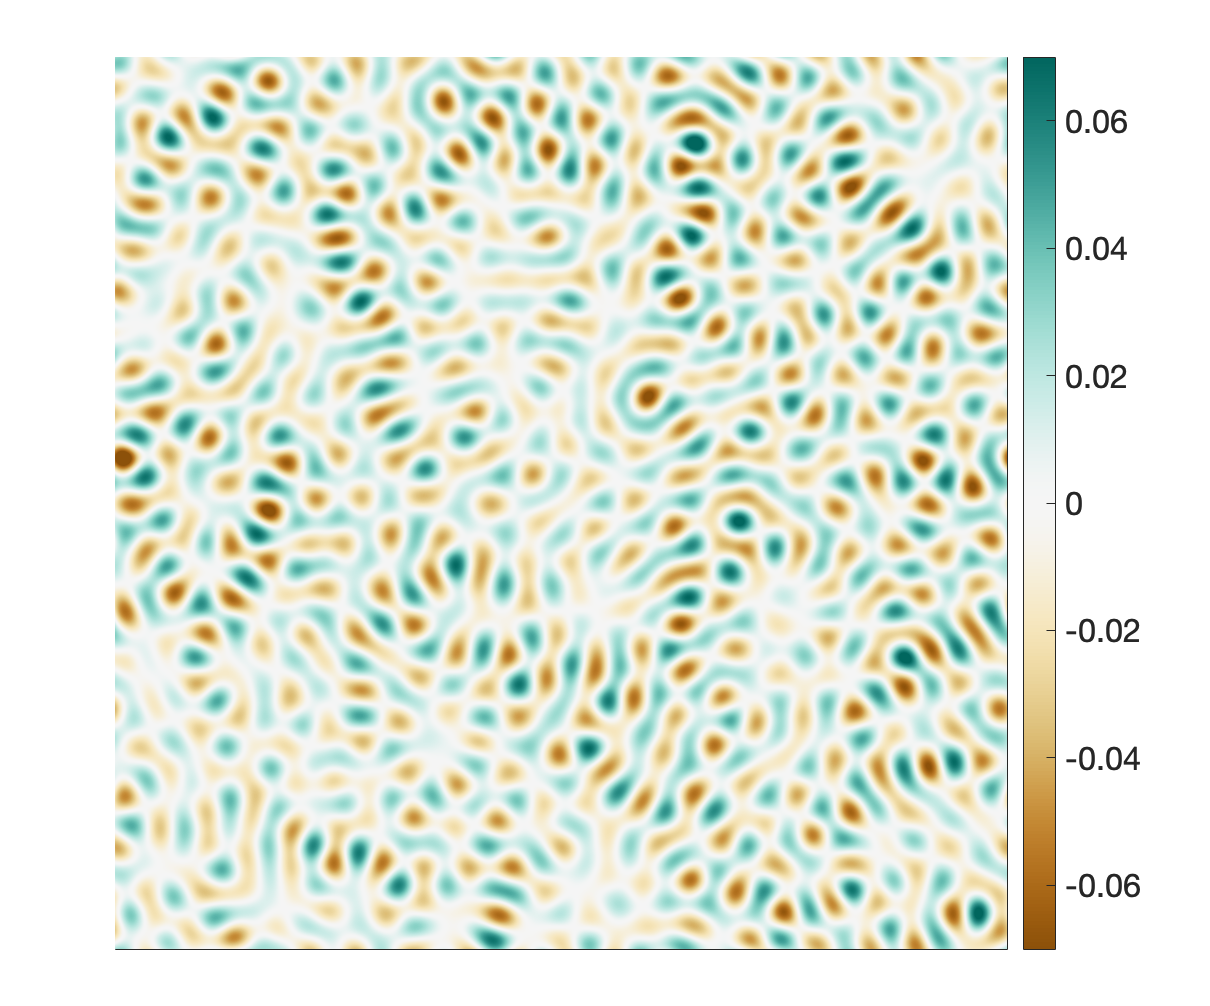
\includegraphics{figures/zr_t0.png}

}

}

\end{minipage}%
%
\begin{minipage}[t]{0.33\linewidth}

{\centering 

\raisebox{-\height}{

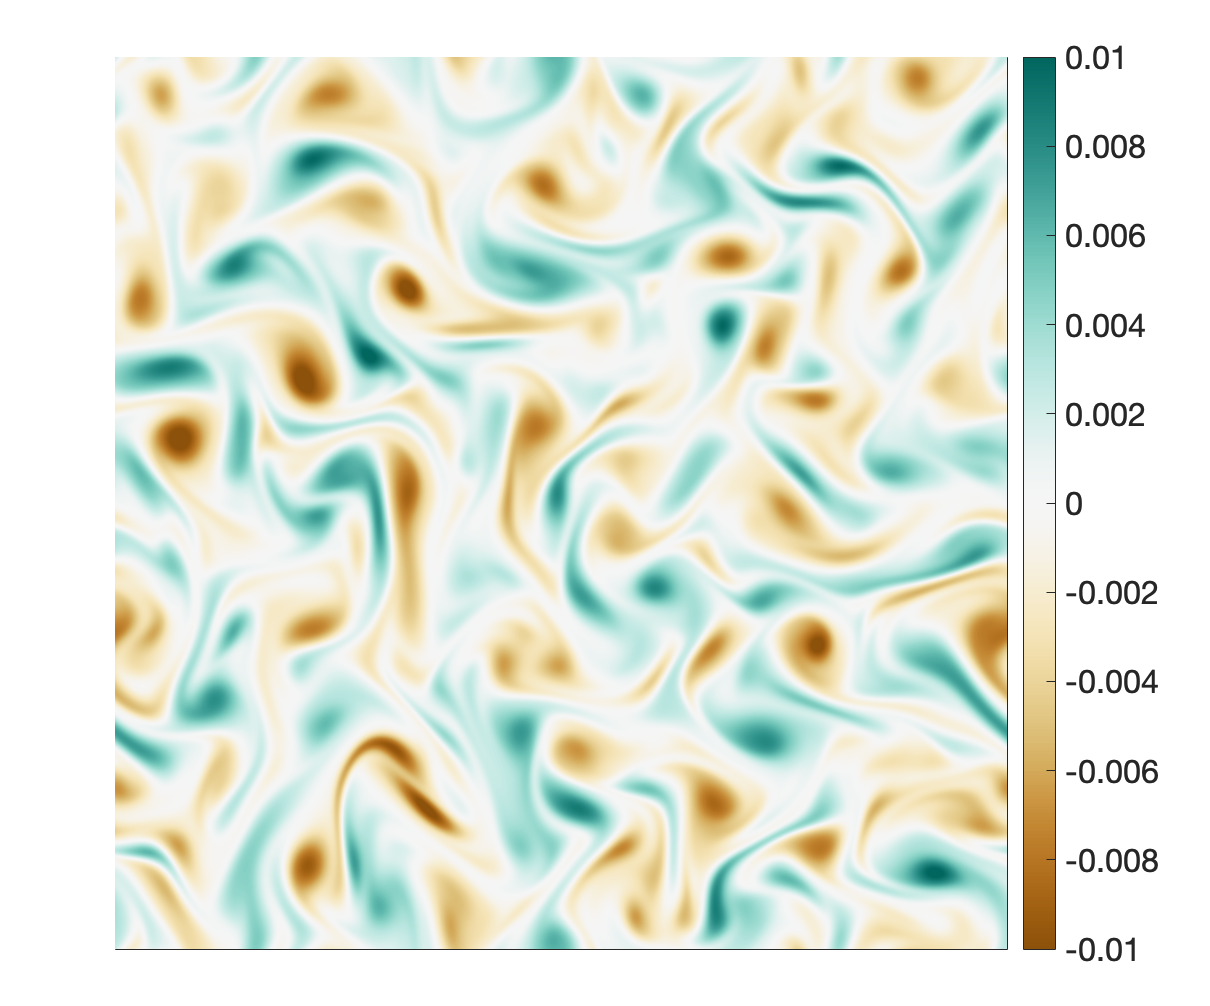
\includegraphics{figures/zr_t4.png}

}

}

\end{minipage}%
%
\begin{minipage}[t]{0.33\linewidth}

{\centering 

\raisebox{-\height}{

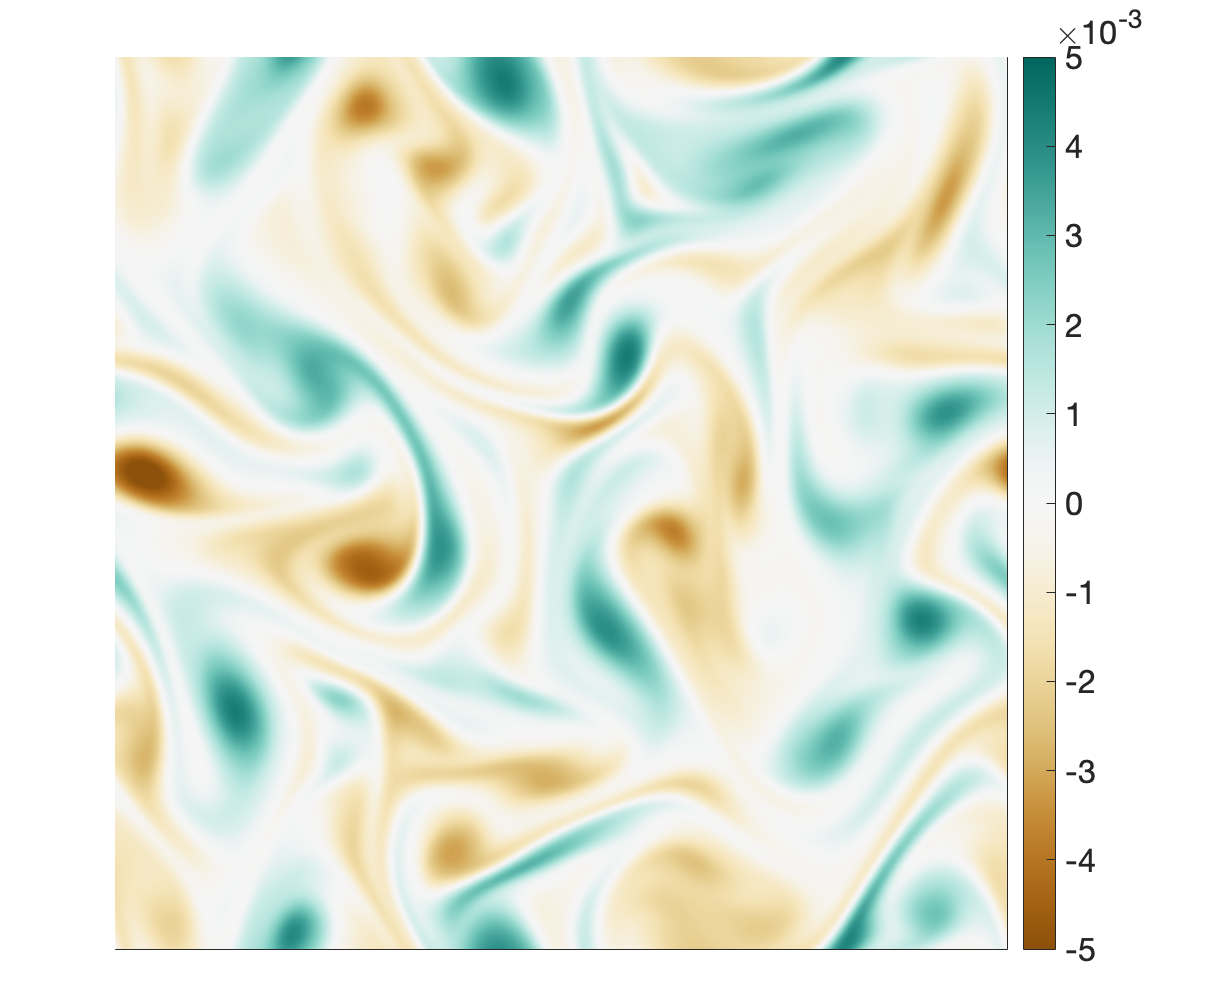
\includegraphics{figures/zr_t10.png}

}

}

\end{minipage}%

\caption{\label{fig-decay}Evolution of a decaying turbulent 2D flow at
initial time (a), intermediate time (b), and the end of the simulation
(c). Colours represent the vorticity field.}

\end{figure}

The flow is then allowed to evolve over time. Figure~\ref{fig-decay}
illustrates the evolution of this flow in physical space at various
times. Initially, the flow's energy is concentrated at smaller vortices,
consistent with the energy spectrum peaking at the intermediate (or
relatively small) scale of \(1/k_i\). Over time, smaller vortices
transfer their energy to larger ones that gradually become the most
energetic structures. This process continues, forming increasingly
larger vortices (see panels (a), (b) and (c) of Figure~\ref{fig-decay}).
This behaviour contrasts sharply with 3D turbulence, where energy
cascades from large to small scales. In 2D turbulence, energy moves from
smaller to larger scales, as evidenced by the energy spectrum's peak
shifting toward smaller wavenumbers (larger scales) over time, as shown
in Figure~\ref{fig-spectra}. This energy transfer to larger scales is
referred to as the \emph{inverse cascade}, distinguishing it from the
forward cascade characteristic of 3D turbulence.

\begin{figure}

{\centering 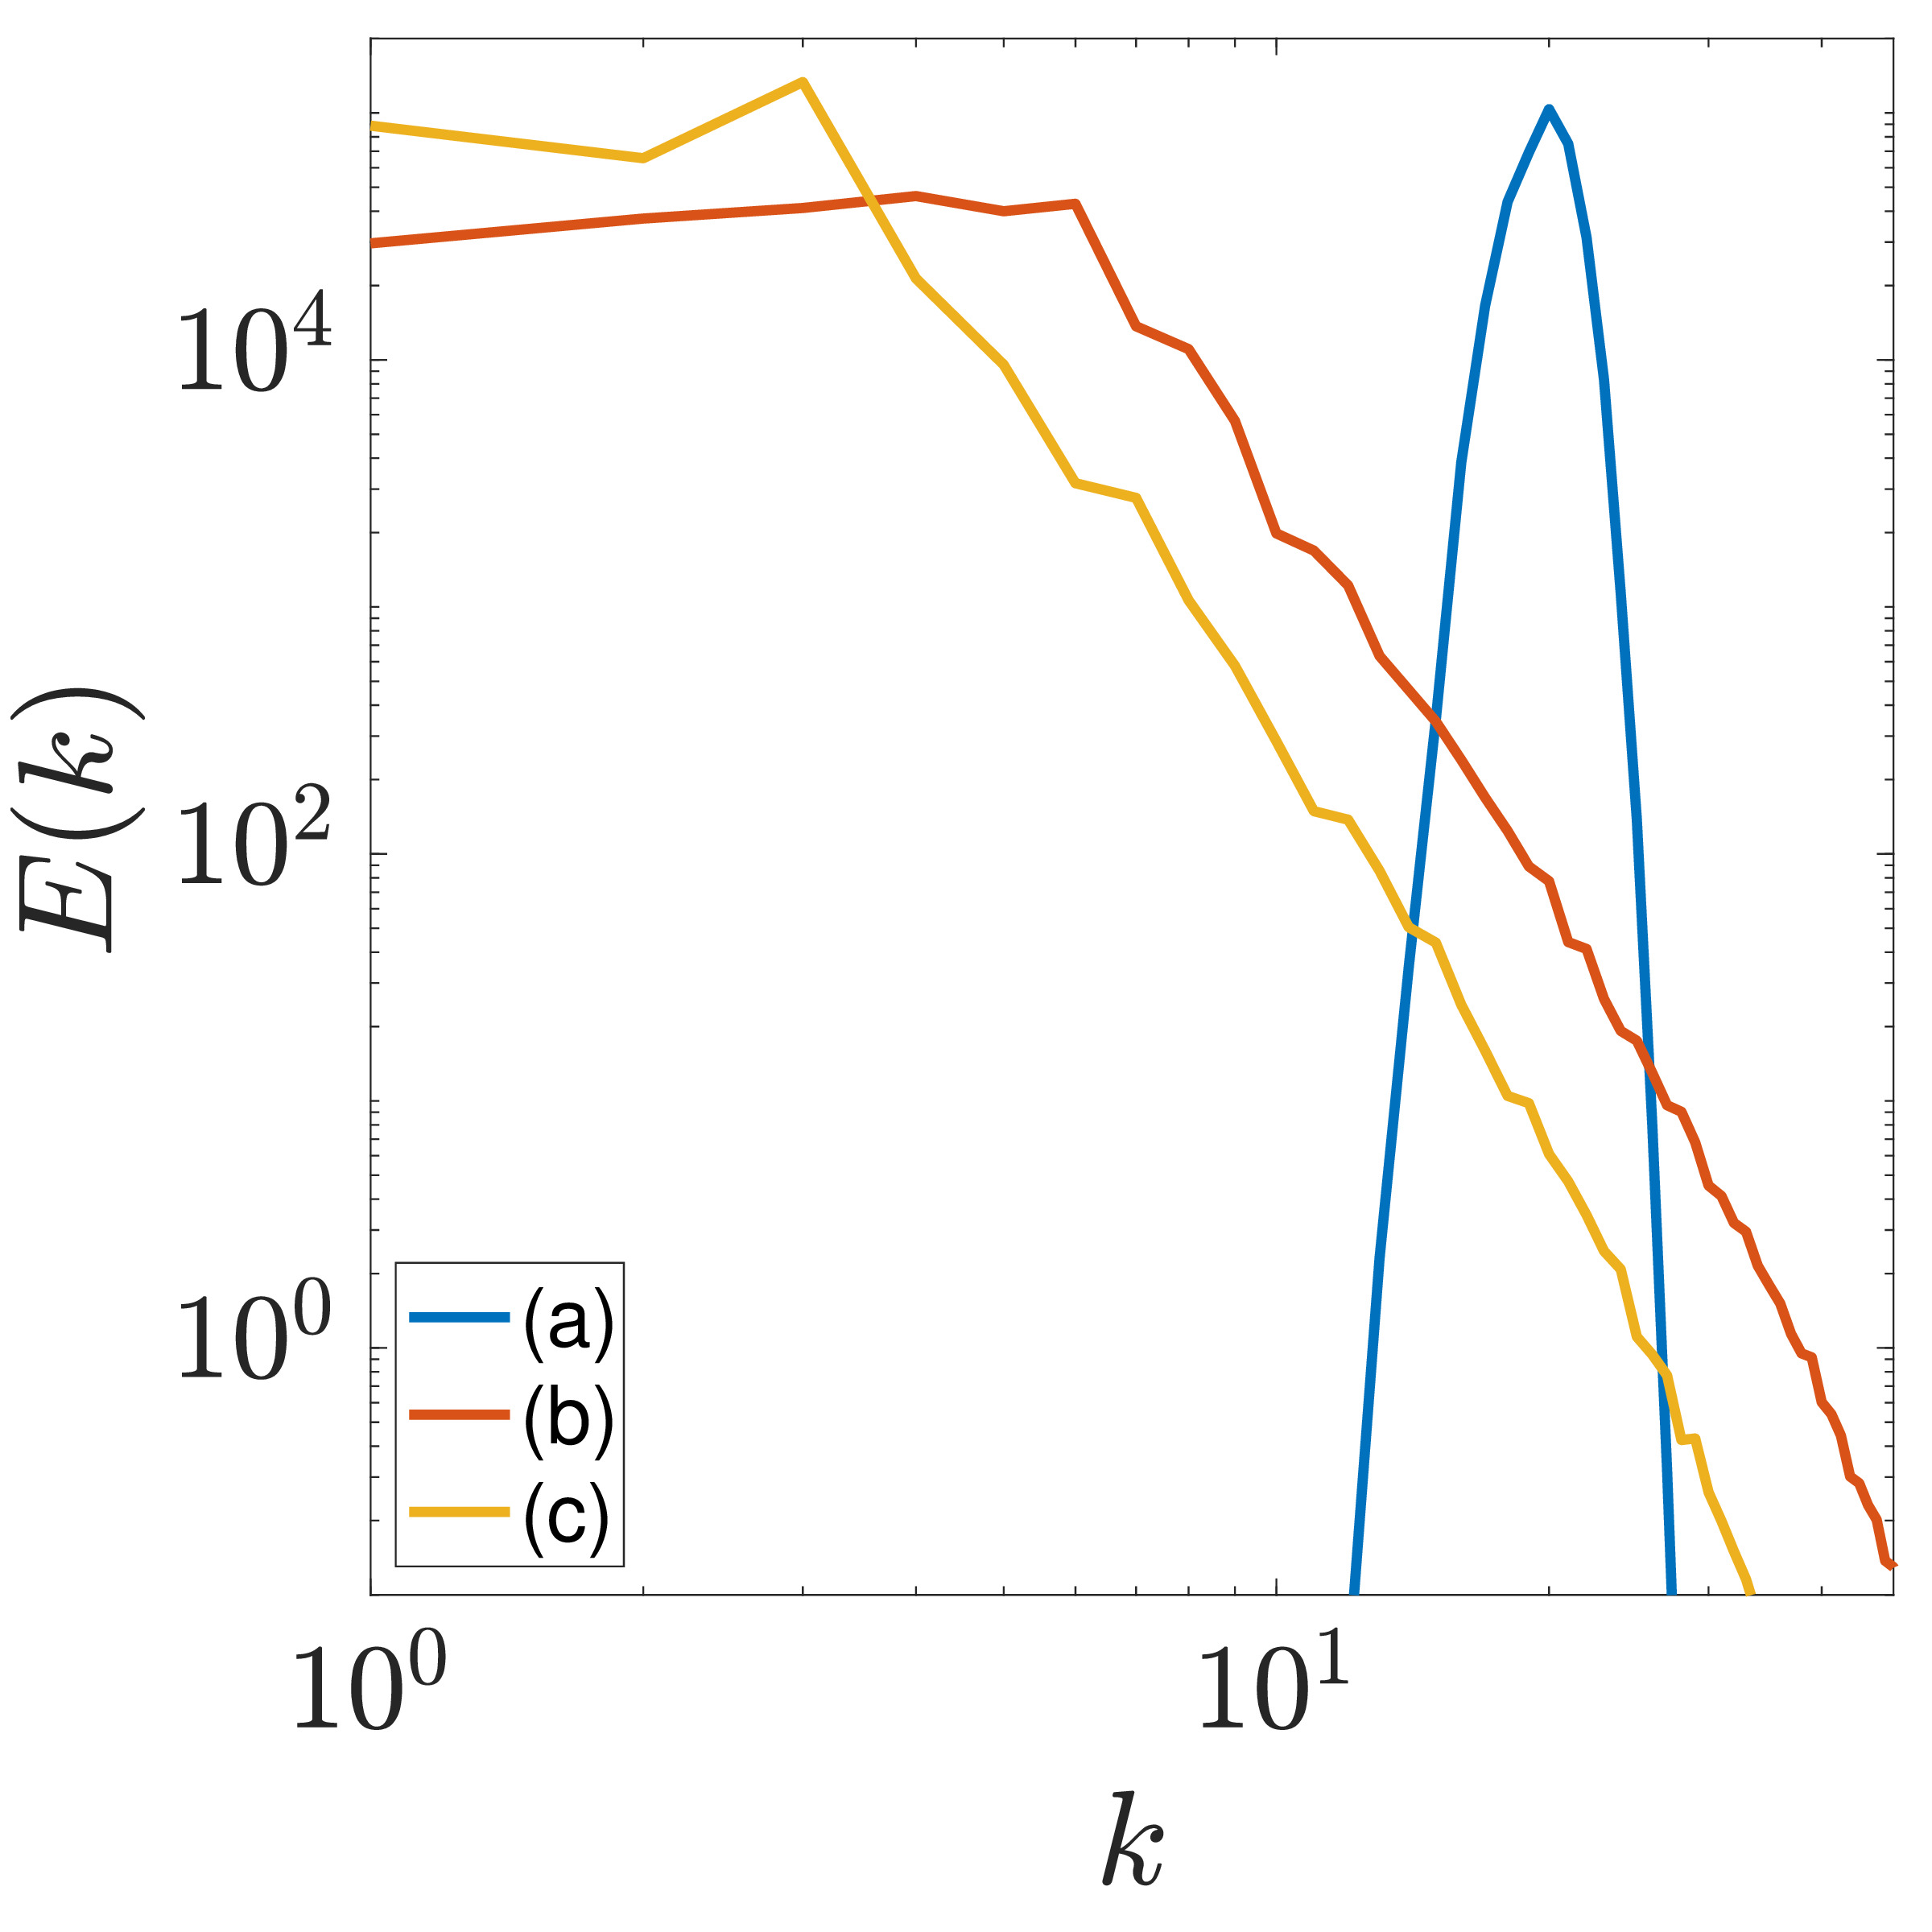
\includegraphics[width=0.45\textwidth,height=\textheight]{figures/energy_spectra.jpg}

}

\caption{\label{fig-spectra}Energy spectra corresponding to the panels
shown in Figure~\ref{fig-decay}.}

\end{figure}

To put these observations on a firmer mathematical foundation, let us
analyze the evolution of energy distribution in wavenumber space. If the
initial energy spectrum is sufficiently narrow, we can define the
characteristic wavenumber of the initial condition \(k_i\) by
\begin{equation}\protect\hypertarget{eq-def_ki}{}{
k_i = \frac{\int k E(k)\, d k}{\int E(k)\, d k}
= \frac{\int k E(k)\, d k}{E_{\text{tot}}}.
}\label{eq-def_ki}\end{equation} We want to see how the spectrum evolves
in time. A fundamental characteristic of turbulence is mixing, which
leads to the spread of this narrow band of energy in wavenumber space.
In other words, due to strong nonlinear interactions in turbulence, the
energy is naturally transferred to other scales. We can quantify the
spreading out of the energy distribution with \[
W = \int (k-k_i)^2 E(k)\, d k,
\] which can be expanded to \begin{align*}
     W = {} & \int k^2 E(k)\, d k - 2 k_i \int k E(k)\, d k + k_i^2 \int  E(k)\, d k \\
     \Rightarrow\quad
     W = {} & Z_{\text{tot}} -  k_i^2 E_{\text{tot}},
\end{align*} where we used Equation~\ref{eq-relateEavrtoEspc},
Equation~\ref{eq-Z_k2E} and Equation~\ref{eq-def_ki} to arrive at the
final expression: \begin{equation}\protect\hypertarget{eq-x1}{}{
W = Z_{\text{tot}} - k_i^2 E_{\text{tot}}.
}\label{eq-x1}\end{equation}

Since energy and enstrophy are conserved in 2D turbulence,
\(d E_{\text{tot}} / d t = d Z_{\text{tot}} / d t = 0\). Then,
differentiating Equation~\ref{eq-x1} with respect to time gives \[
\frac{d k_i^2}{d t} = -\frac{1}{E_{\text{tot}}} \frac{d W}{d t}.
\] The spreading of the initial narrow energy band implies
\(dW/dt > 0\), leading to \(d k_i^2/d t < 0\). Thus, \(k_i\) decreases
over time, indicating that the typical length scale of vortices
increases, consistent with the numerical results shown in
Figure~\ref{fig-decay}.

\begin{figure}

{\centering 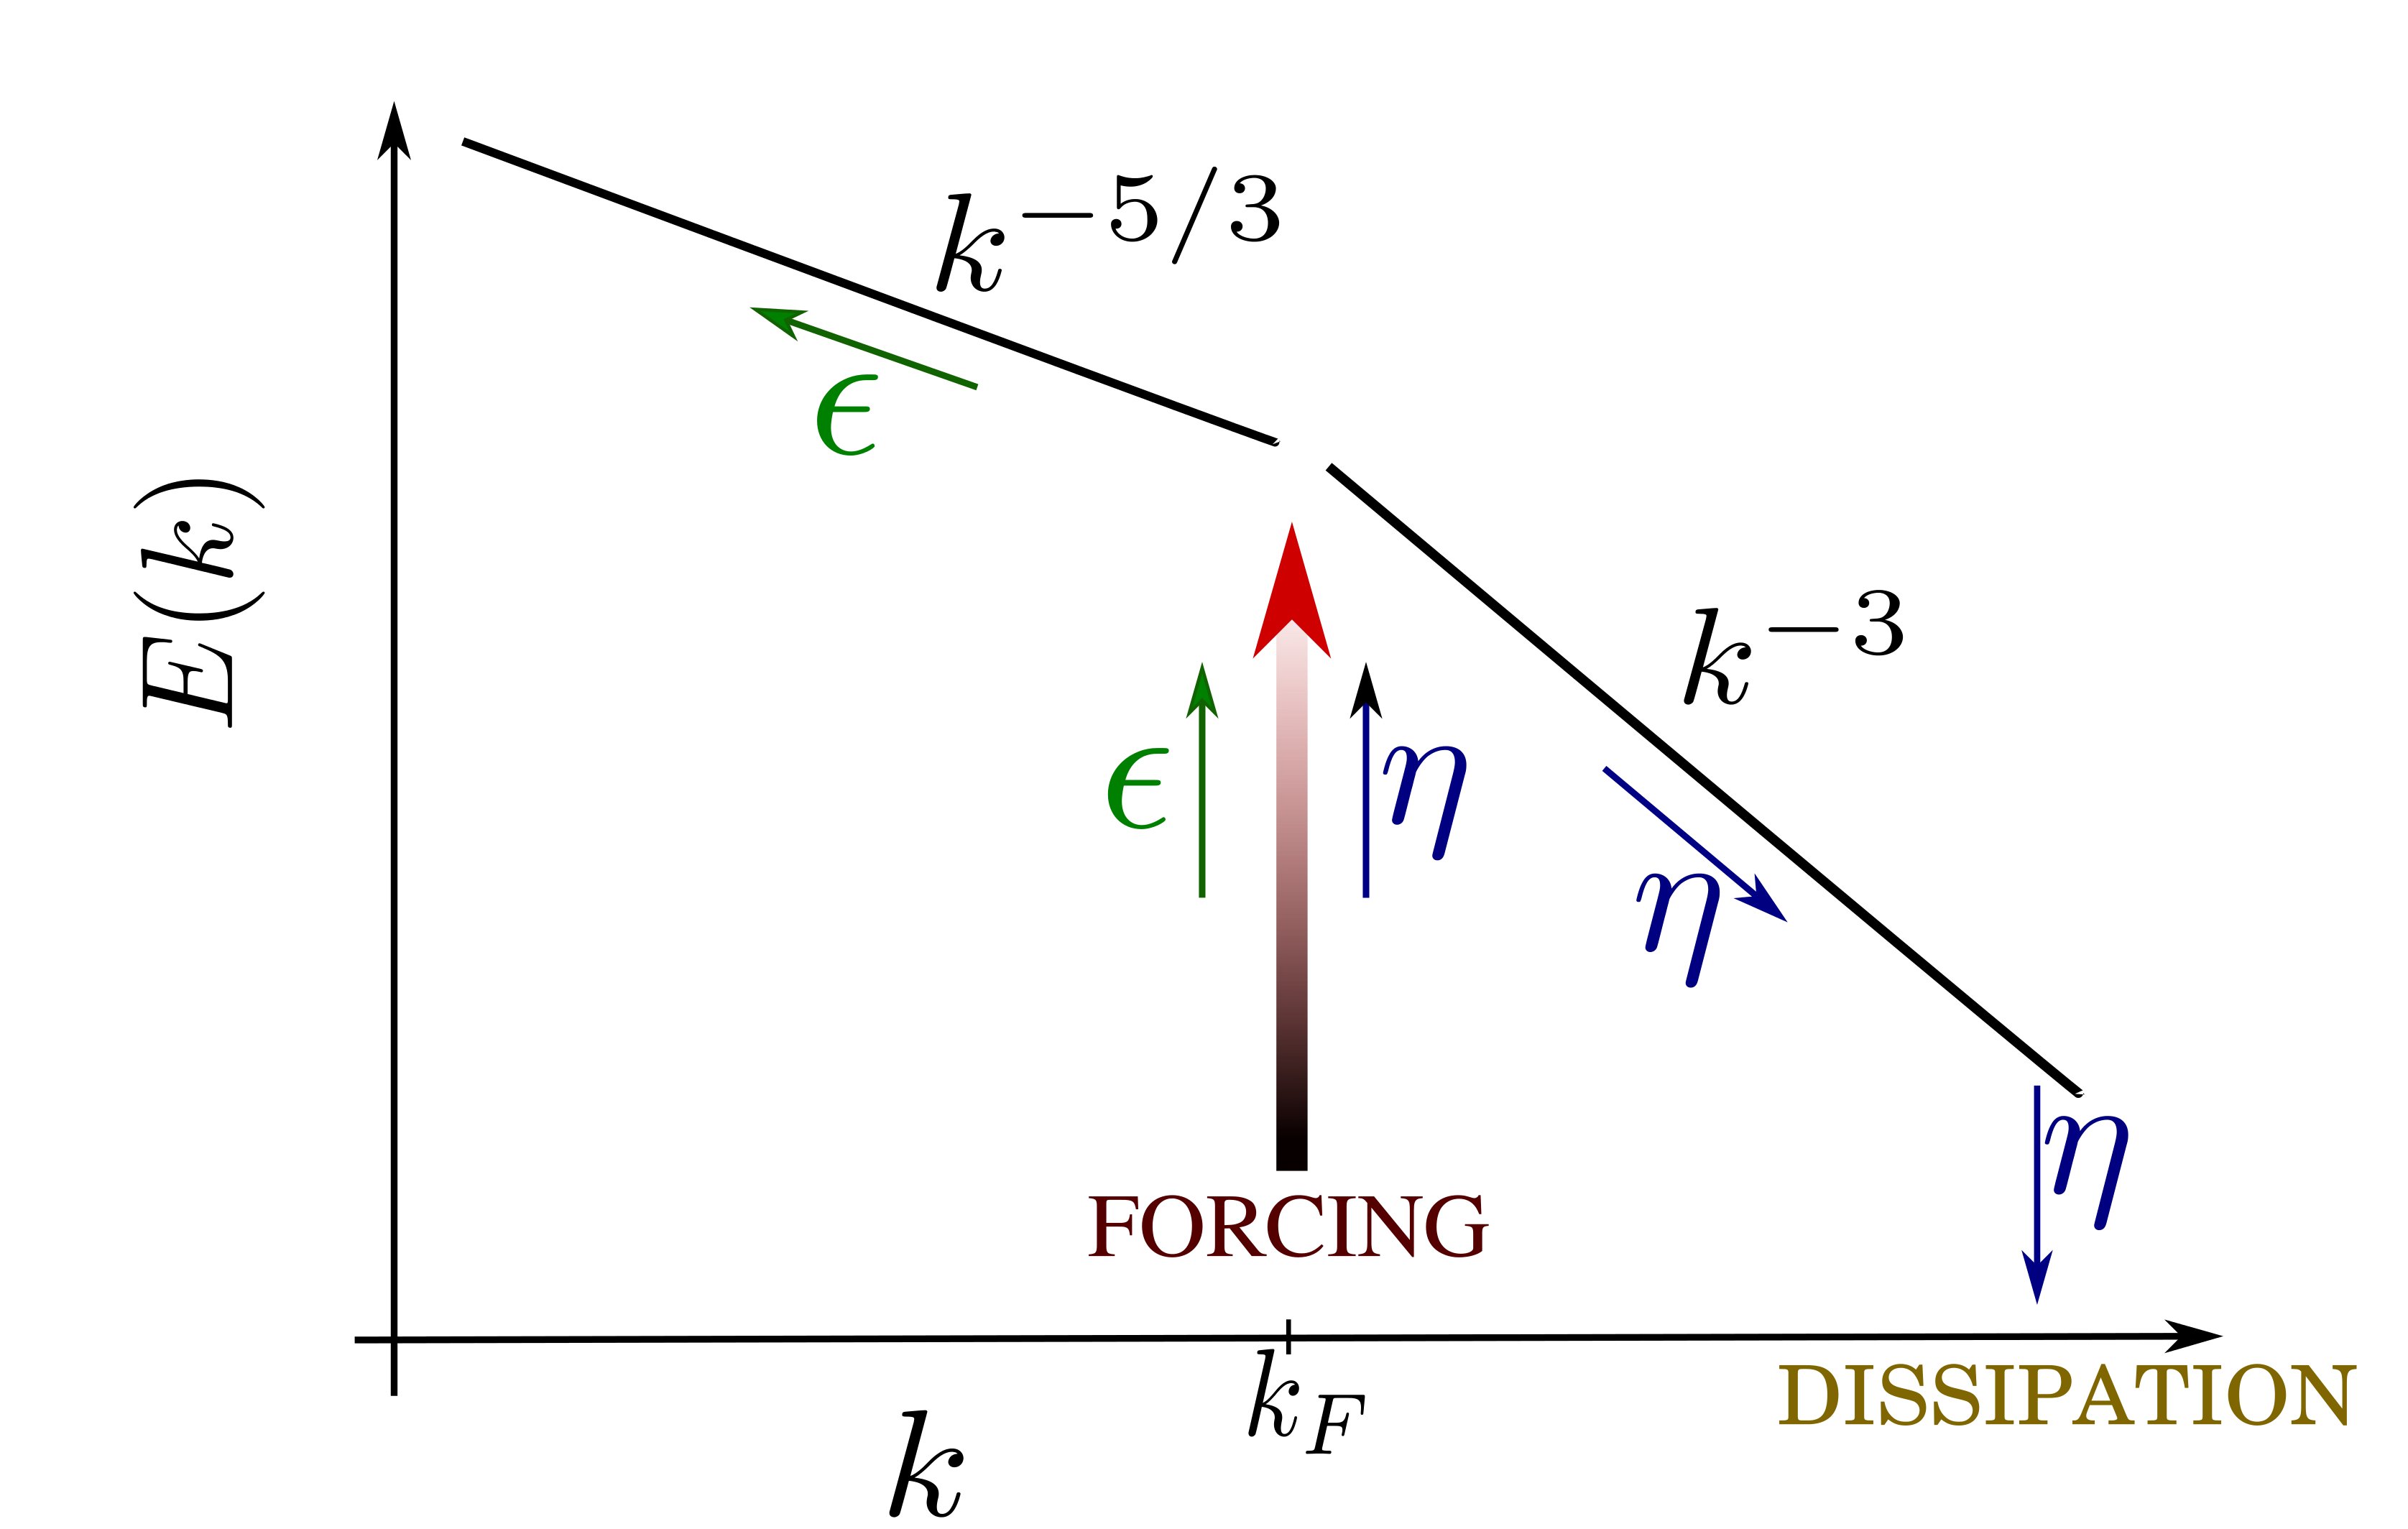
\includegraphics[width=0.6\textwidth,height=\textheight]{figures/turbulence2Dcascades.png}

}

\caption{\label{fig-cascades2D}Energy spectrum of 2D turbulence with
both forward cascade of enstrophy and inverse cascade of energy.}

\end{figure}

Now, let us return to the forced problem, equipped with the insight that
energy in 2D turbulence is transferred to larger scales. If the flow is
forced at an intermediate scale \(k_F\), we expect energy to cascade
upscale for \(k < k_F\), resulting in an energy spectrum following
Equation~\ref{eq-EnergySubrange}. Conversely, enstrophy, which is also
conserved in 2D flows, must cascade downscale for \(k > k_F\) (as its
flux cannot co-exist with energy flux in the range of \(k < k_F\)),
leading to an energy spectrum consistent with
Equation~\ref{eq-EnstrophySubrange}. This behaviour, known as the double
or dual cascade, is depicted schematically in
Figure~\ref{fig-cascades2D}, where the cascade directions and the
corresponding slopes of spectra are shown.

This picture of forced 2D turbulence is commonly referred to as the
\emph{Kraichnan--Batchelor} theory, named after the two prominent
scientists who developed it. To achieve the statistical stationarity
assumed in Equation~\ref{eq-EnergySubrange}, a mechanism must dissipate
energy at scales much larger than the forcing scale. A plausible
physical mechanism is the scale-independent dissipation characteristic
of Ekman layers near boundaries as long as their effects remain
negligible within the inertial range.

\hypertarget{sec-geoturb}{%
\section{Geostrophic turbulence}\label{sec-geoturb}}

The seminal paper by Charney (1971) established the theory of
geostrophic turbulence. The motivation stemmed from a paradox:
observational spectra showed a \(k^{-3}\) slope at large atmospheric
scales---consistent with 2D turbulence---yet the atmosphere is clearly
not two-dimensional in this regime.

The theory relies on the QG system introduced in
Section\textasciitilde{}Chapter~\ref{sec-Geostrophic}, which accurately
describes large-scale atmospheric and oceanic flows. For simplicity,
assume constant \(N\) and \(f\). The total QG energy, consisting of
horizontal kinetic plus available potential energy, is
\begin{equation}\protect\hypertarget{eq-consEinQG}{}{
E_{\text{tot}}
= \frac{1}{\mathtt{V}}\int_{\mathtt{V}}
\left( u^2 + v^2 + \frac{b^2}{N^2} \right) d\xb
= \frac{1}{\mathtt{V}}\int_{\mathtt{V}}
\left( |\nabla\psi|^2 + \frac{f^2}{N^2} \psi_z^2 \right) d\xb.
}\label{eq-consEinQG}\end{equation}

The QG potential vorticity,
\begin{equation}\protect\hypertarget{eq-PVrep}{}{
q = \zeta + \frac{f_0}{N^2} \frac{\partial b}{\partial z}
= \nabla_H^2\psi + \frac{f_0^2}{N^2}\psi_{zz},
}\label{eq-PVrep}\end{equation} is materially conserved,
\begin{equation}\protect\hypertarget{eq-QGdim2}{}{
\frac{Dq}{Dt} = \frac{\partial q}{\partial t} + \vb\cdot\nabla_H q = 0,
}\label{eq-QGdim2}\end{equation} implying conservation of
\emph{potential enstrophy},
\begin{equation}\protect\hypertarget{eq-consZinQG}{}{
Z_{\text{tot}} = \frac{1}{\mathtt{V}}\int_{\mathtt{V}} q^2\, d\xb.
}\label{eq-consZinQG}\end{equation}

QG flow is neither 2D nor 3D isotropic. To make its invariants resemble
those of 2D turbulence, Charney proposed a vertical coordinate
stretching: \[
\tilde{z} = \frac{N}{f} z.
\]

In the stretched coordinate, Equation~\ref{eq-QGdim2} becomes
\begin{equation}\protect\hypertarget{eq-QGeqNewCor}{}{
\frac{\partial}{\partial t}\nabla^2_\ast\psi
+ u\,\frac{\partial}{\partial x}\nabla^2_\ast\psi
+ v\,\frac{\partial}{\partial y}\nabla^2_\ast\psi = 0,
}\label{eq-QGeqNewCor}\end{equation} where \[
\nabla_\ast = \left(\frac{\partial}{\partial x},
                 \frac{\partial}{\partial y},
                 \frac{\partial}{\partial \tilde{z}}\right)
\] is an isotropic gradient operator. The energy and potential enstrophy
become \begin{equation}\protect\hypertarget{eq-EcharneyCor}{}{
\mathsf{E}_{\text{geo}} = \int |\nabla_\ast\psi|^2\, d\xb,
}\label{eq-EcharneyCor}\end{equation} and
\begin{equation}\protect\hypertarget{eq-ZcharneyCor}{}{
\mathsf{Z}_{\text{geo}} = \int (\nabla_\ast^2\psi)^2\, d\xb.
}\label{eq-ZcharneyCor}\end{equation}

These have the same mathematical form as the 2D energy and enstrophy
invariants, except that \(\nabla_H\) has been replaced by
\(\nabla_\ast\) and the integrals are now three-dimensional.

Therefore, the same arguments that apply to 2D turbulence apply to QG
turbulence in the stretched coordinates. In particular, potential
enstrophy cascades forward, and the associated energy spectrum in the
``synoptic'\,' range is
\begin{equation}\protect\hypertarget{eq-QGEnsSubrange}{}{
E(\tilde{k}) = C_{\text{geo}}\,\eta^{2/3}\,\tilde{k}^{-3},
}\label{eq-QGEnsSubrange}\end{equation} where
\(\tilde{k} = (k_x^2 + k_y^2 + (f/N)^2 k_z^2)^{1/2}\).

Assuming isotropy in \(\nabla_\ast\) space, the kinetic and potential
energy components, \[
E_x,\; E_y,\; E_{\tilde{z}},
\] each inherit the same \(k^{-3}\) slope. Transforming back to physical
coordinates implies that both horizontal kinetic and available potential
energy spectra in the atmosphere follow this \(-3\) scaling.

\hypertarget{sec-atmosspc}{%
\section{Atmospheric energy spectrum}\label{sec-atmosspc}}

We now illustrate how turbulence theories explain the observed
atmospheric energy spectrum. Figure~\ref{fig-GageNastrom}, taken from
Nastrom and Gage 1985, is a landmark observational result covering a
broad range of scales, obtained from over \(6000\) commercial aircraft
flights in the Global Atmospheric Sampling Program (GASP). Later studies
using improved datasets reproduced similar spectra.

In the synoptic range (corresponding to wavelengths up to roughly
\(500\,\mathrm{km}\)), the zonal velocity, meridional velocity, and
potential temperature all exhibit a \(k^{-3}\) slope. This is precisely
the scaling predicted by geostrophic turbulence theory in the
forward-cascading enstrophy subrange
(Section\textasciitilde{}Section~\ref{sec-geoturb}). Because \(E_x\),
\(E_y\), and \(E_{\tilde{z}}\) all share the same \(k^{-3}\) slope, the
consistency across all three observed spectra supports the applicability
of QG dynamics at synoptic scales.

At wavelengths smaller than \(500\,\mathrm{km}\), the spectrum
transitions sharply to a shallower \(k^{-5/3}\) slope (sometimes
interpreted as \(-2\)). While the \(k^{-3}\) regime is well-understood,
the physical explanation of the \(k^{-5/3}\) range remains an active
area of research.

\begin{figure}

{\centering 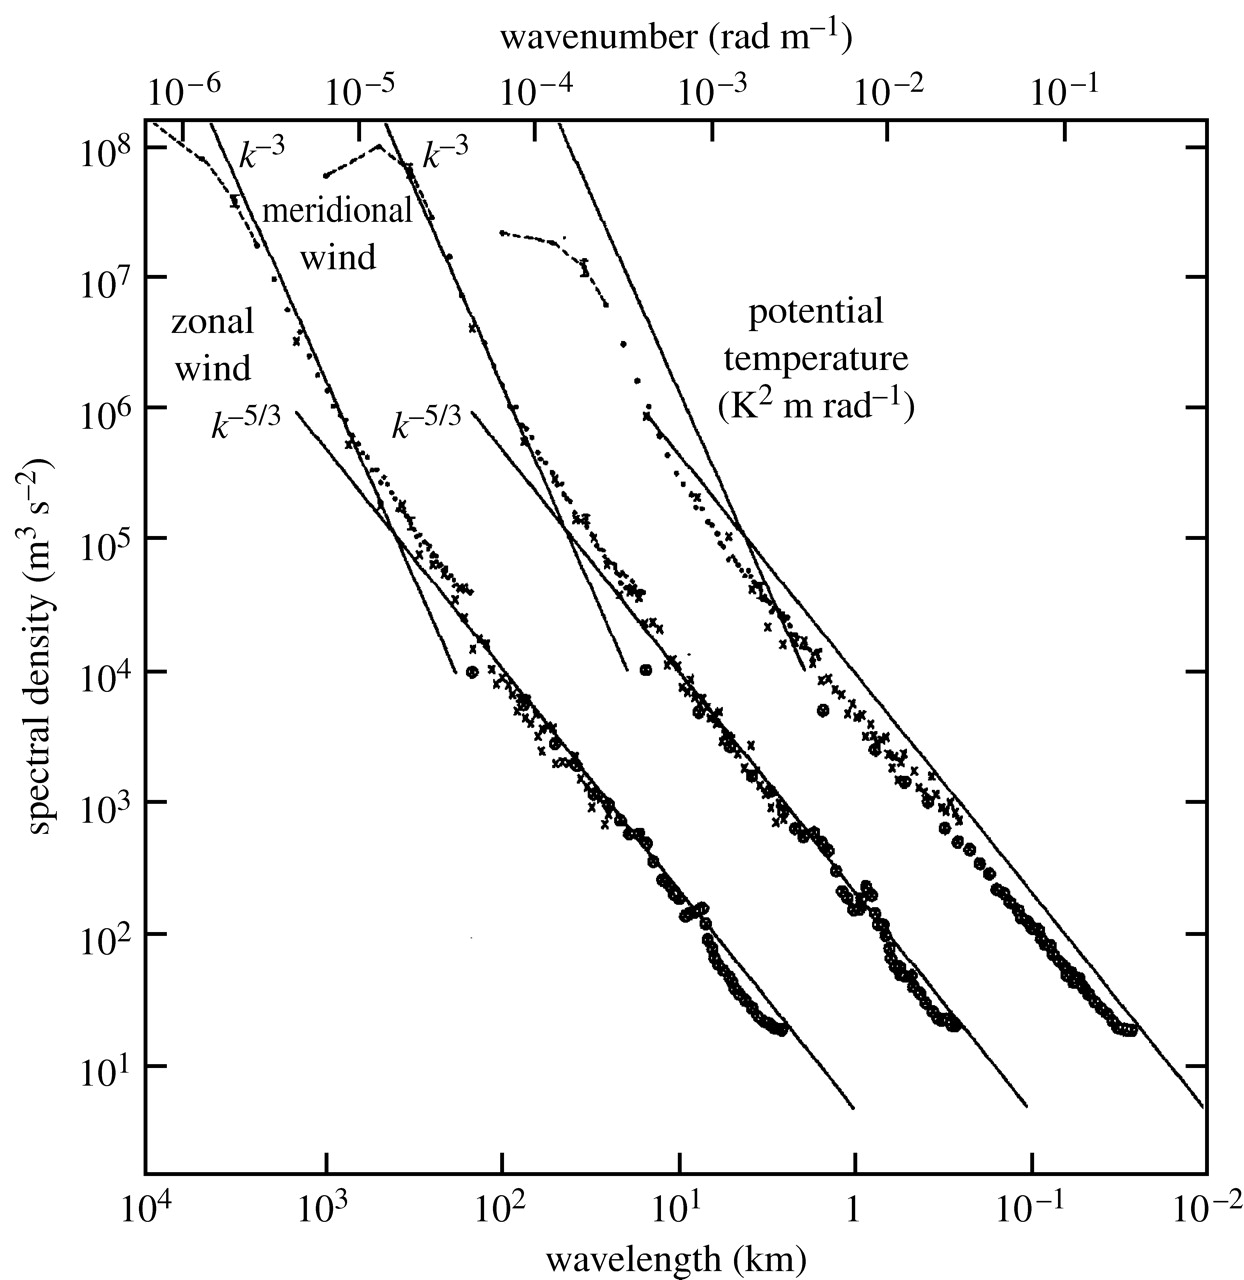
\includegraphics[width=0.6\textwidth,height=\textheight]{figures/NastromGageSpc.jpg}

}

\caption{\label{fig-GageNastrom}Wavenumber spectra of zonal (\(u\)) and
meridional (\(v\)) velocities and potential temperature. Dashed lines
indicate slopes of \(-3\) and \(-5/3\). For visual clarity, the \(v\)
and \(\theta\) spectra are horizontally shifted by one and two decades,
respectively.}

\end{figure}



\end{document}
